% !TEX options=--shell-escape
\documentclass[a4paper,12pt]{article}
% \usepackage[legalpaper, portrait, lmargin=2in,rmargin=1in]{geometry}
\usepackage{verbatim}
\usepackage{fixltx2e}
\usepackage{amsmath, amssymb, amsfonts}
\usepackage{booktabs}
\usepackage[dvipsnames]{xcolor}
\usepackage[margin=30mm]{geometry}
\usepackage{graphicx}
\usepackage{pdfpages}
\usepackage{listings}
\usepackage{xcolor}
\usepackage[hidelinks]{hyperref}
\usepackage{setspace}
\usepackage{booktabs}
\usepackage{footnote}
\newcommand{\ra}[1]{\renewcommand{\arraystretch}{#1}}
% \doublespacing
\onehalfspacing

\definecolor{codegreen}{rgb}{0,0.6,0}
\definecolor{codegray}{rgb}{0.5,0.5,0.5}
\definecolor{codepurple}{rgb}{0.58,0,0.82}
\definecolor{backcolour}{rgb}{0.95,0.95,0.92}

\lstdefinestyle{mystyle}{
    backgroundcolor=\color{backcolour},   
    commentstyle=\color{codegreen},
    keywordstyle=\color{magenta},
    numberstyle=\tiny\color{codegray},
    stringstyle=\color{codepurple},
    basicstyle=\ttfamily\footnotesize,
    breakatwhitespace=false,         
    breaklines=true,                 
    captionpos=b,                    
    keepspaces=true,                 
    numbers=left,                    
    numbersep=5pt,                  
    showspaces=false,                
    showstringspaces=false,
    showtabs=false,                  
    tabsize=2
}

\lstset{style=mystyle}


\graphicspath{
{../img}
}
% \usepackage{svg}
\usepackage{hyperref}
% \usepackage{cite}

\usepackage[style=numeric]{biblatex}
\addbibresource{REPORT.bib}
% \hypersetup{
% colorlinks=true,
% linkcolor=blue,
% filecolor=blue,{}
% urlcolor=blue,{}
% citecolor=black
% }

\usepackage{soul}
\usepackage{url}
% \usepackage{siunitx}
\usepackage{tikz}
\usepackage{minted}
\newcommand{\jwj}[1]{{\color{red}{~(jwj: #1)}}}
\newcommand{\yourInitials}[1]{{\color{blue}{~(yourInitials: #1)}}}
\usepackage{xcolor} % to access the named colour LightGray
\definecolor{LightGray}{gray}{0.9}
\font\Huge=cmr12 at 20pt
\usepackage{fancyhdr} 
\begin{document}

\pagestyle{fancy}
\renewcommand{\chaptermark}[1]{\markboth{#1}{#1}}
\fancyhead[R]{}
\fancyhead[L]{\chaptername\ \thechapter\\ \leftmark}

\clearpage
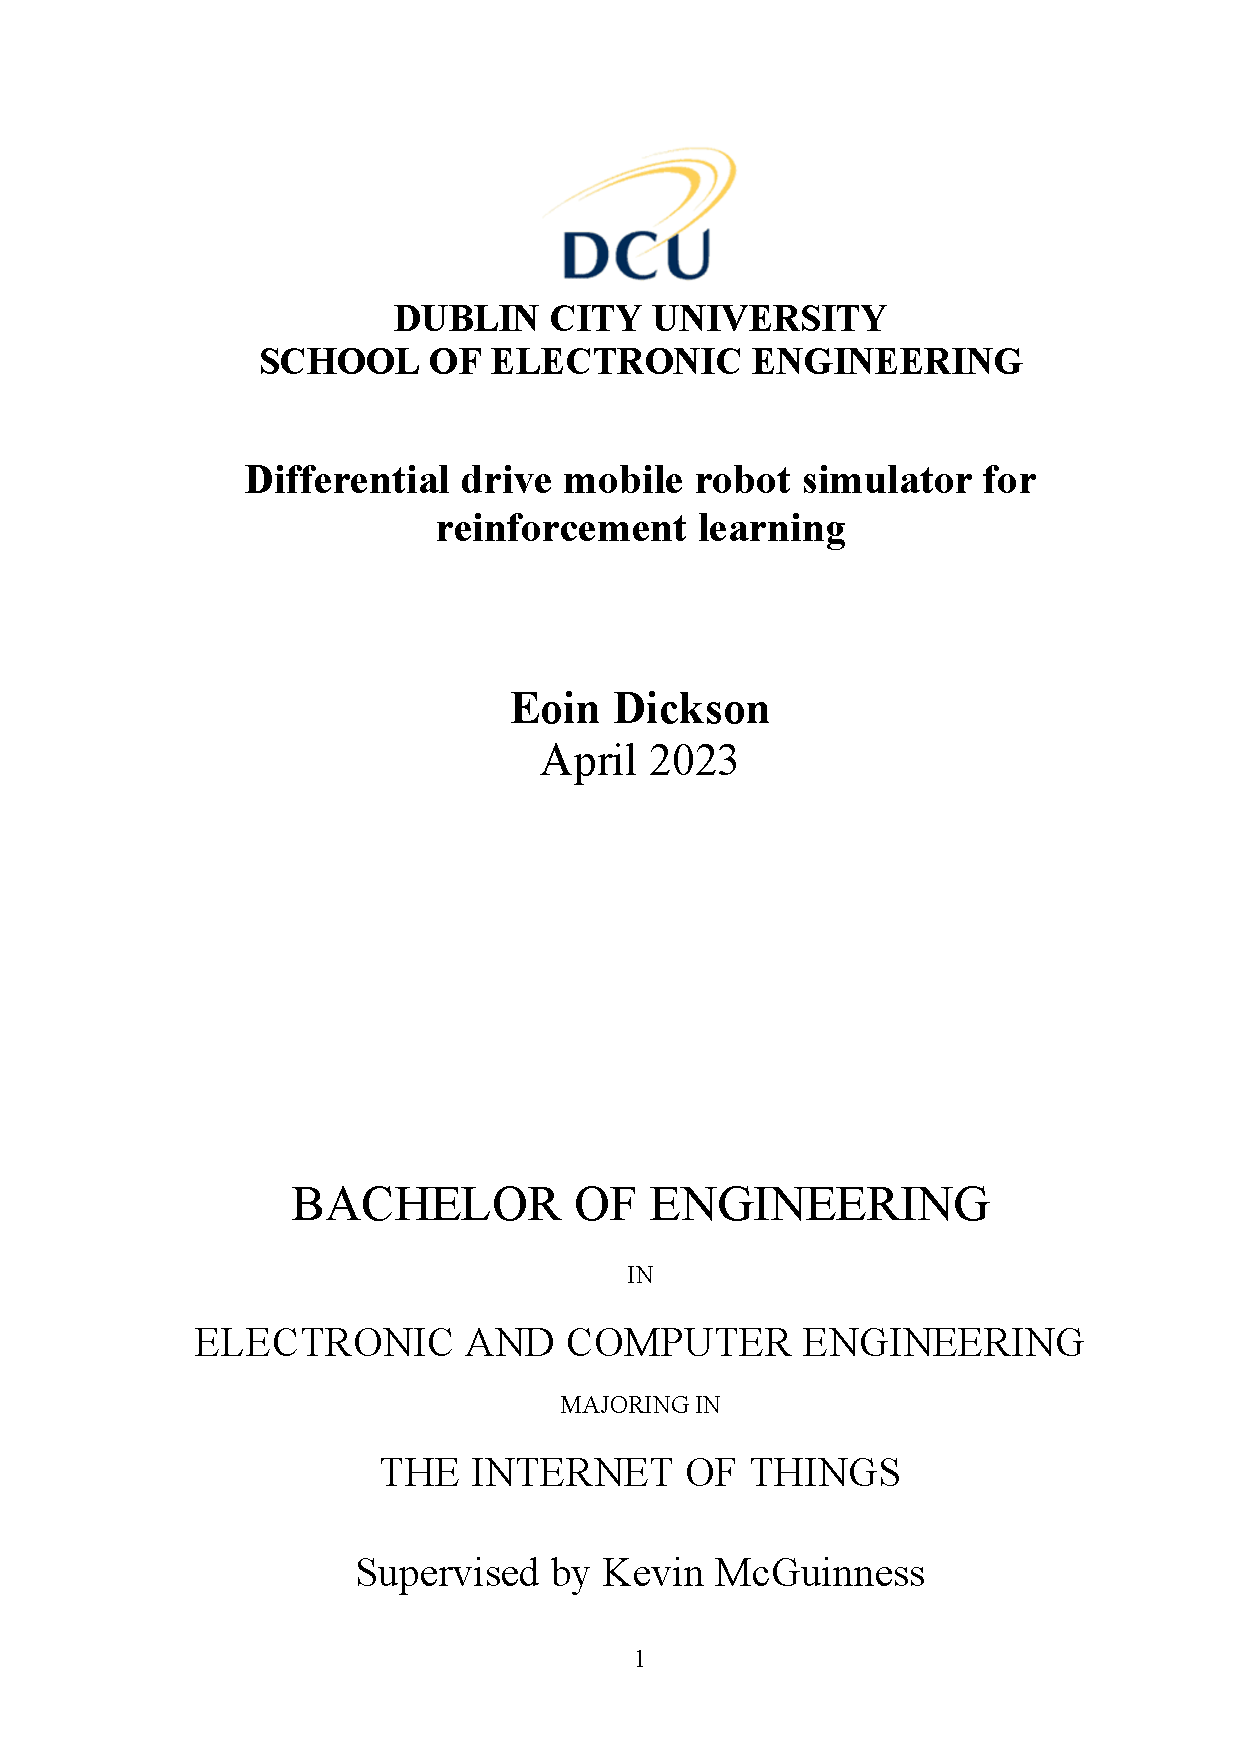
\includepdf[pages=-]{FrontPage.pdf}

\section{Abstract}
This project aimed to develop a simulator for a differential drive line following robot with the goal of using it for reinforcement learning. The simulator was built using OpenAI Gym, a reinforcement learning toolkit, and PyGame, a two-dimensional game development platform. State-of-the-art reinforcement learning algorithms from StableBaselines were used to train a neural network. The hardware and the track from EE303 Moblie Robotics were used for the foundations of the simulator. The simulator successfully trained a model using Proximal Policy Optimization and a discrete action space. The trained neural network was ported to EE303's hardware using C. The robot and the simulator were extensively tested using visual testing, TensorBoard and verification testing. Further areas of development were outlined, such as object detection using machine vision and the implementation of other features from EE303 mobile robotics.


% This project was to develop a simulator for a differential drive line following robot. The simulator was used for reinforcement learning and was developed using OpenAI Gym. State-of-the-art reinforcement learning algorithms from StableBaslines were used to train a neural network. The hardware and the track from EE303 Mobile Robotics were the basis of the simulator. Once trained the neural network was ported to the EE303 hardware using C. The robot was tested both on and off the track and future areas of study were outlined.
% \\\\
% This project aims to develop a simulator for a differential drive line following robot. The simulator will be used for reinforcement learning and developed using OpenAI Gym. State-of-the-art reinforcement algorithms from StableBaslines will be used to train a neural network. The hardware and the track from EE303 Mobile Robotics will be the basis of the simulator. Once trained, the neural network will be ported to the EE303 hardware using C. The robot will be tested, and a road map of future steps needed for functionality will be outlined.
\pagebreak

% This report presents a project that aims to develop a simulator to train a differential drive robot to follow a line. The simulator will be developed using OpenAI Gym a reinforcement toolkit, it will be able to follow a track with complex turns and intersections such as the track from EE303. This simulator will be trained using reinforcement learning algorithms to verify the environment and to obtain a model for porting. The trained model will be ported to the EE303 robot's hardware to research the future steps needed to get the robot functioning properly. 


\tableofcontents


\pagebreak
\listoffigures
\pagebreak
\listoftables
\pagebreak

\section{Introduction}
\subsection{Motivation}

With more and more technologies such as reinforcement learning, machine learning and artificial intelligence becoming more commonly used in our daily life, this raises some questions. How can we integrate such technologies into our projects? Can these technologies improve human-made systems? How do we train these technologies?
\\\\
Throughout our formal education in university, we are initially taught how to programme starting with the basics. We are gradually taught more and more complex programming skills, and the above technologies are discussed but have yet to be discovered in much detail. As these technologies are being used more broadly, getting as much hands-on experience as possible is essential.
\\\\
This project intends to take a previous module studied, EE303 Mobile Robotics which aims to teach students to code control algorithms, solve integration issues and ultimately create a differential drive line following robot capable of following a complex track; to develop a simulator for reinforcement learning that will allow this robot to follow a line. This simulator will allow other students to get an introduction to training neural networks using reinforcement learning and to allow the students to use this simulator to get a better understanding how it can be implemented into projects they are completing.

\subsection{Current Systems}

Traditional systems are usually based upon a set of rules, and control loops and these rules are then programmed using programming techniques \cite{lakshmanababu2022exploring}. An engineer will approach a problem, explore all the different aspects that affect the system and create a set of rules. Once these sets of rules are created, then they would be programmed using if statements, case statements and other techniques to create the system.
\\\\
In the context of the line follower robot, the robot uses five sensors arranged horizontally across the front of the robot. Some sample logic created by an engineer would be that if the line is detected under the far-left sensor, the robot should turn to the left to avoid moving off the line. This logic would be coded using a simple if statement to make the robot turn left.

\subsection{Problems with Current Systems}

The traditional systems demonstrated above, although they at first seem to be very logical, they have their flaws. These styles of systems are rigid in their approach, and they will stay the same as their environment changes. They also get exponentially more complex along with more complex problems.
\\\\
The rigidity of these traditional systems can be seen when you are testing or training your system. With these systems, you must recode and alter your code to change the robot's functionality and performance. The use of reinforcement can make these changes without outside help. Some examples of problems that can only be solved using reinforcement learning are chess and Go. These are both highly complex board games that have an almost infinite amount of moves and scenarios. Through the use of reinforcement learning an agent can be developed to play these games at a high level.  
\\\\
The complexity of these systems can be demonstrated by using a similar example to the above. The robot should turn to the left if the leftmost sensor is on the line. If the robot uses history as an input, then the logic goes from a simple if statement to a more complex algorithm.


\subsection{Reinforcement Learning System}

Systems created using reinforcement learning are entirely based on policies that are learned from experience, simulation and iteration from training. These control systems can be non-linear dynamic systems, which gives them a large advantage \cite{dev2021machine}. The correct setup of observation, action and reward spaces can give a system that humans would be incapable of coming up with. Failure to implement these spaces correctly can lead to a failed system. Reinforcement learning is best for designing complex systems such as natural language processing, video games and robotics, and this is because of its iterative nature. These systems are often very effective once trained, although if left unsupervised can become stuck in suboptimal solutions. If a line following robot finds a suboptimal solution it could be zigzagging across the line rather than smoothly following it.

\section{Background}
\subsection{EE303 Mobile Robotics}

EE303 Mobile Robotics is a third-year engineering module at Dublin City University. This module aims to teach students to create a functioning differential drive line following robot. Differential drive robots are very convenient for control and have high mobility \cite{bakirci2022kinematics}. This robot should have the following functionality, the ability to follow a track with intersections and complex curves, the ability to navigate from location to location dictated by a track map and a fixed start position and orientation, and the robot should also communicate to a web server to receive and send current locations.
\\\\
The hardware from EE303 is vital to understanding how to approach this problem. The hardware includes two DC motors, one on each side of the cylindrical robot and a caster wheel near the front. Controlling the two motors independently allows robots to manoeuver well and to work well in an indoor environment. Mobile robots with such drive systems are a typical example of non-holonomic mechanisms due to the perfect rolling constraints on a wheel motion (no longitudinal or lateral slipping) \cite{Malu}. These three elements are the components that allow for the robot's movement. 
\\\\
The next essential components are the sensing components. These are limited to two types of sensors the array of five photodiode sensors located horizontally at the very front of the robot and the distance sensor located directly above. To tie all the components together, an MSP432 \cite{msp432} microcontroller is used along with its Wi-Fi board to process and communicate. The Wi-Fi board and the distance sensor are unnecessary for the line following functionality. The robot can be seen in \autoref{fig:Robot}.
\\\\
\begin{figure}[H]
\centering
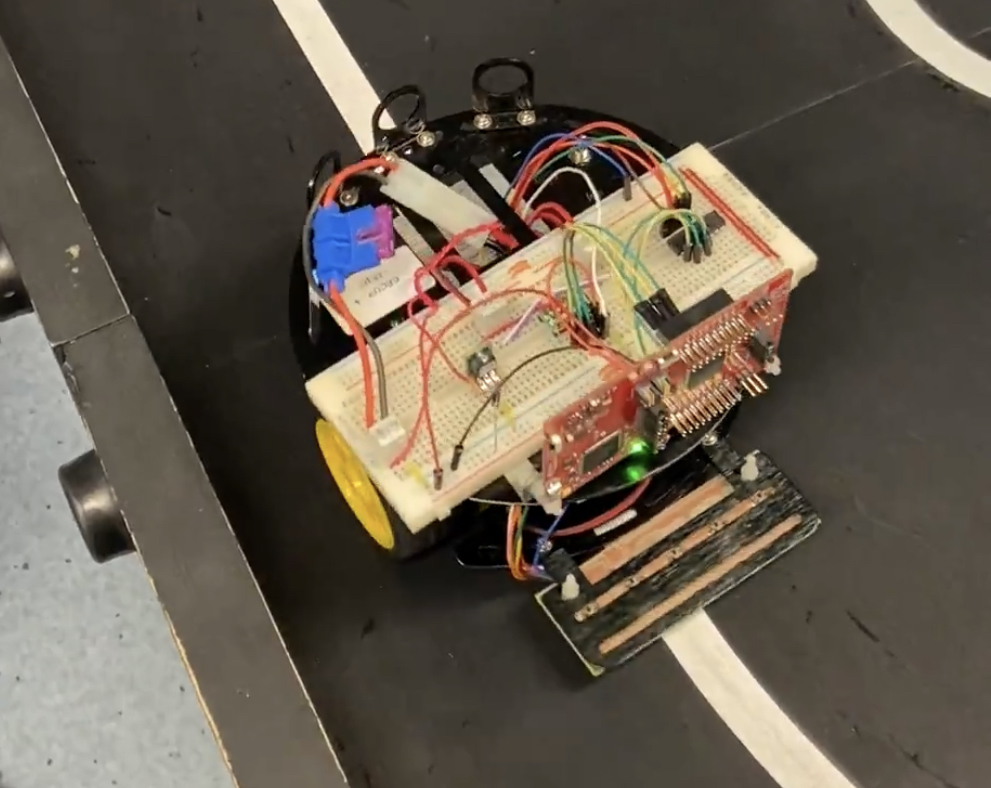
\includegraphics[width=10cm]{imgs/Robot.jpg}
\caption{The robot from EE303. This includes the two DC motors, microcontroller and sensor array.}
\label{fig:Robot}
\end{figure}
\noindent
The main functionality of this model and the objective this module aims to address is the ability of a student to create a robot capable of following a complex track. This map can be seen below. The map is based on a black background with white electrical tape as the line. Each of the different locations on the track can be seen, although will are not necessary for the line following functionality. The track layout including the location numbers can be seen in \autoref{fig:TrackWNumbers}.
\\\\
\begin{figure}[H]
\centering
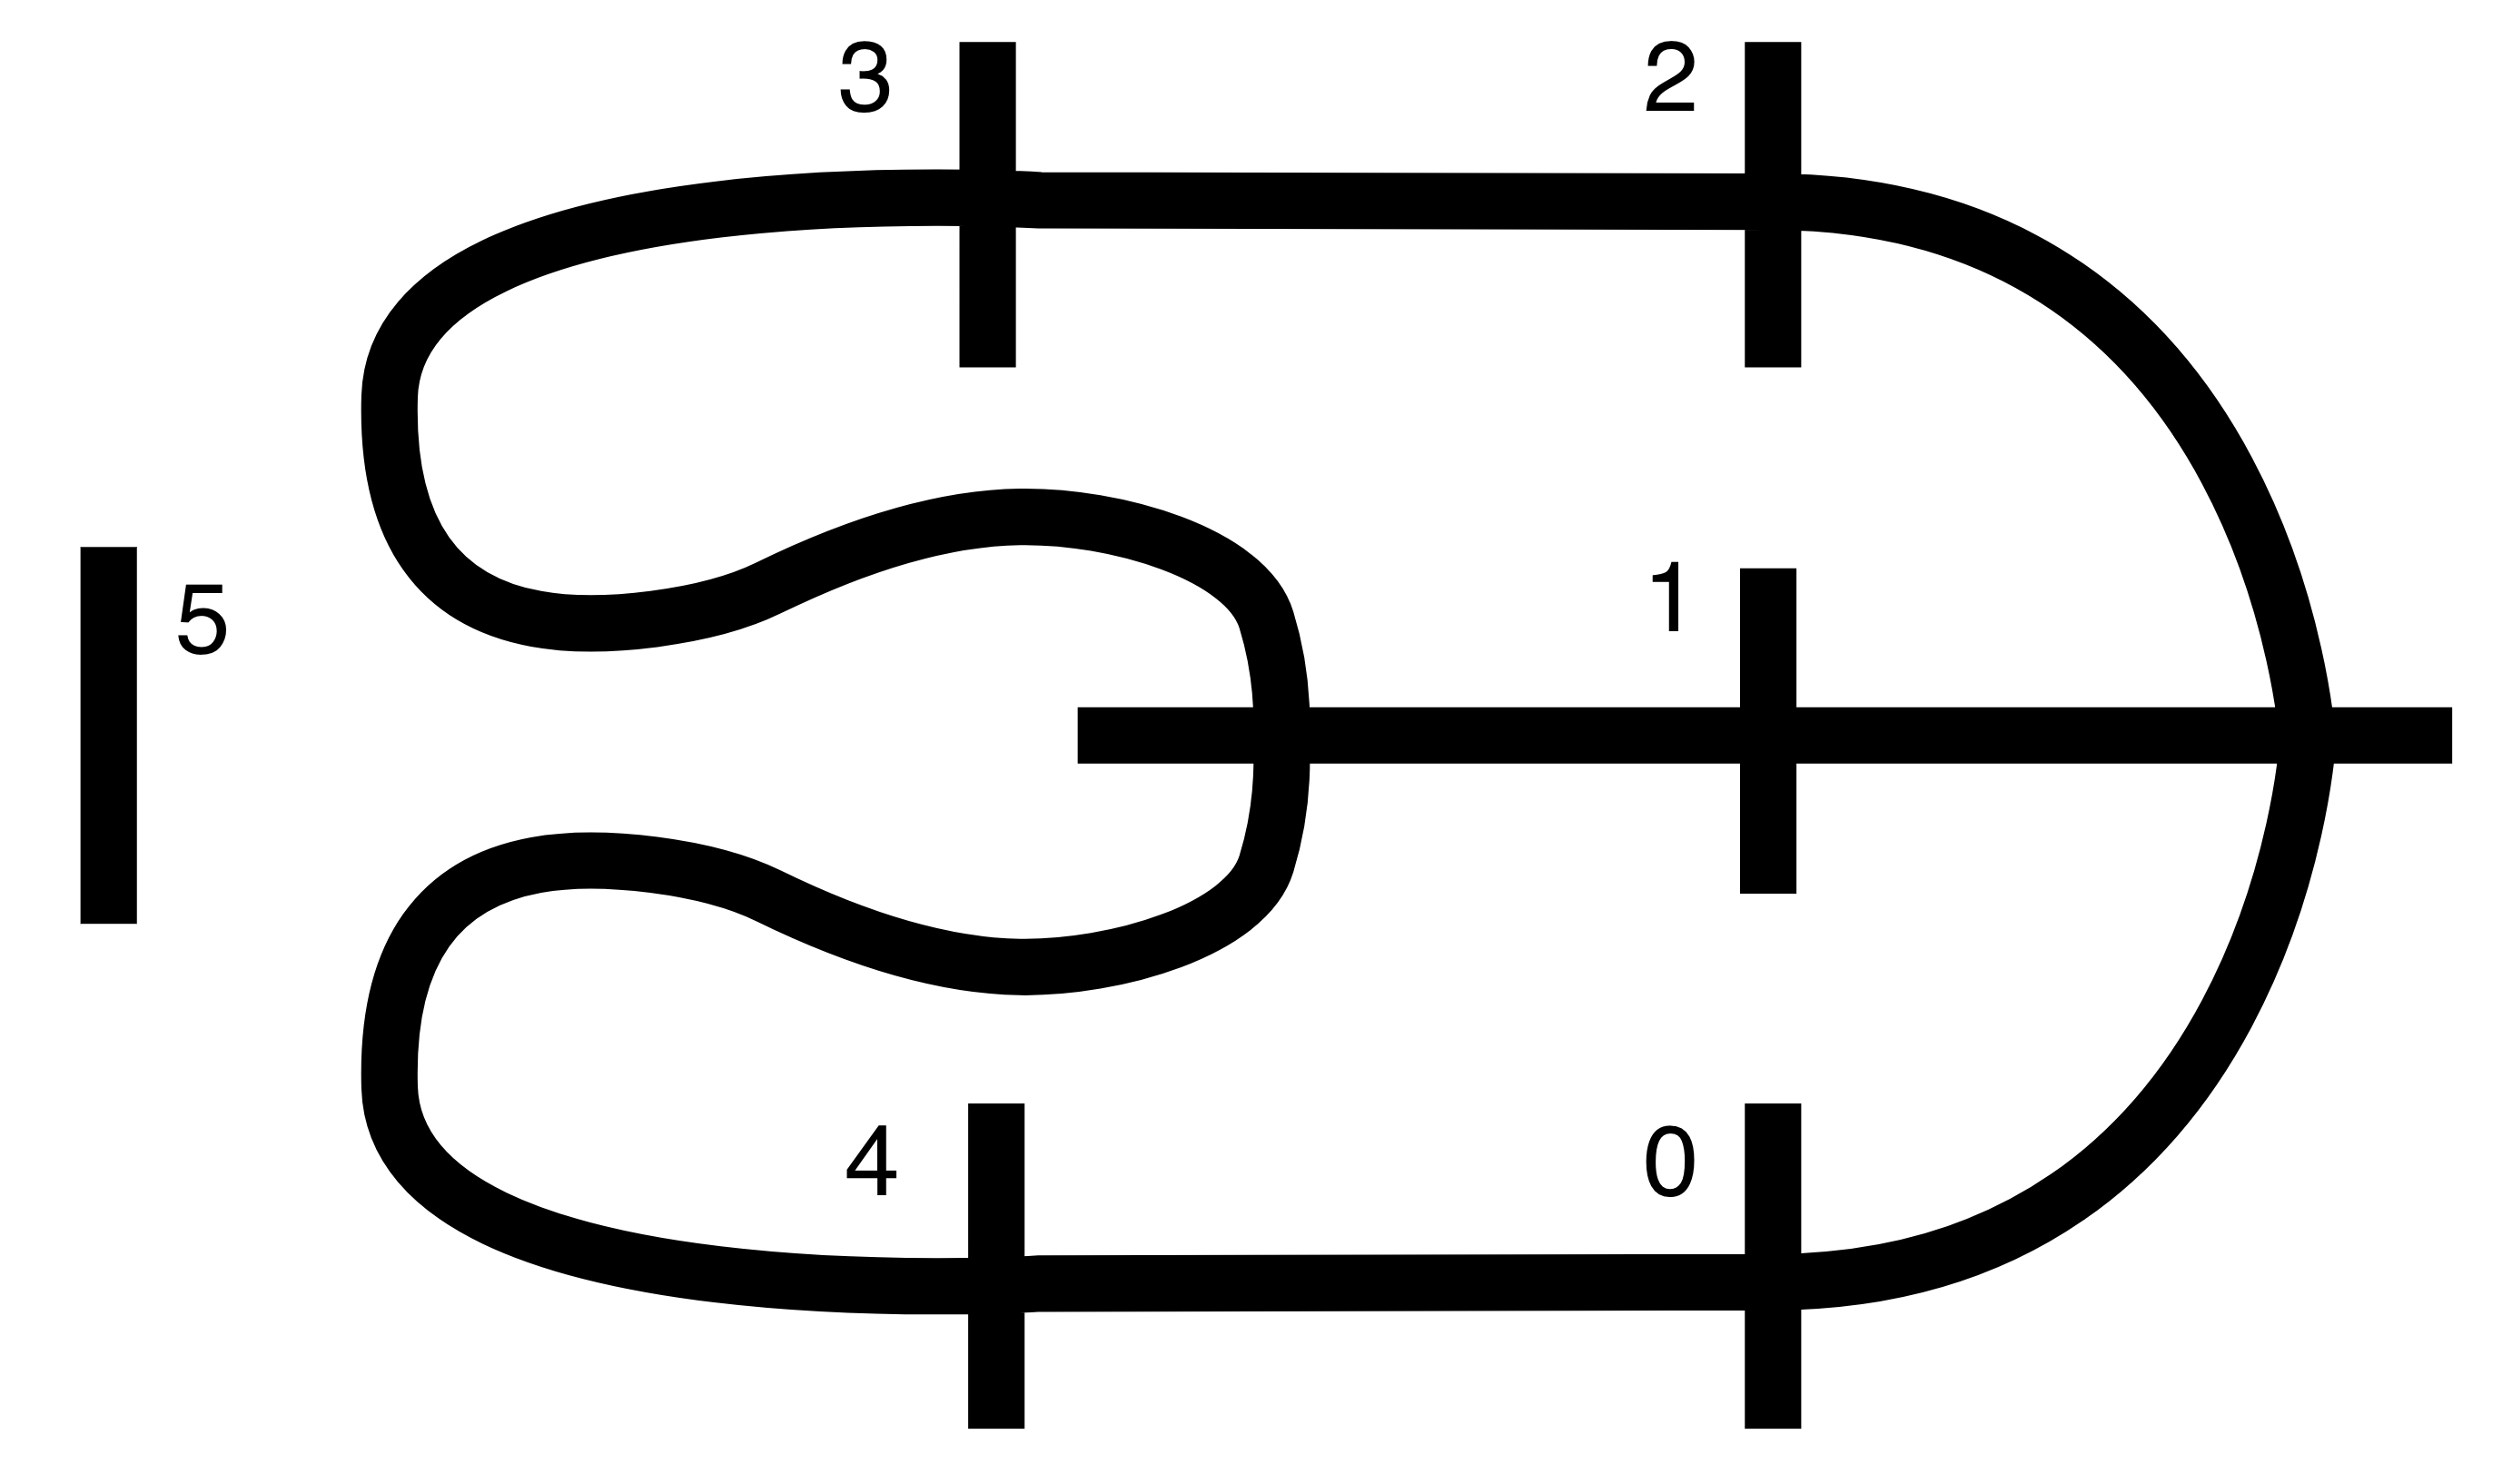
\includegraphics[width=10cm]{imgs/TrackWNumbers.png}
\caption{The track from EE303 web server showing the complex radii, intersections and location numbers \cite{KevinMcGuinness}}
\label{fig:TrackWNumbers}
\end{figure}

\subsection{Reinforcement Learning}

What is reinforcement learning? Reinforcement learning is learning what to do-how to map situations to actions so as to maximise a numerical reward signal. The learner is not told which actions to take but is left to its own actions and must discover which actions yield the most reward by trying them \cite{sutton1992introduction}. Reinforcement learning of a couple main concepts, agent, environment, state, action, reward, policy and value function.
\\\\
The agent is the entity that interacts and makes actions based on the information given. An agent can be viewed similarly to a player; a player receives information from a video game and then uses their knowledge to make an action.
\\\\
The environment is the real-world or simulated environment in which the agent operates. An environment could be as simple as an Atari game, such as asteroids, or it could be the real world where a robot has to pick up or move an object from one location to another. The agent will be situated in these environments to learn; this makes it essential that the environments are as close to the final environment as to minimise porting issues and so that there is little difference between its training environment.
\\\\
The state is the current status that the agent perceives; it contains all of the information about the environment that the agent has access to. This information could be location, orientation, velocity, or other object's locations. The state is all the information that an agent has to decide on its next action.
\\\\
Actions can be classified into two categories, discrete and continuous actions. Discrete actions are a set of actions that are predefined and can be chosen. An example of discrete actions could be forward and backwards; there are two discrete actions only in this case.
\\\\
Continuous actions are that allow their value to be any value between a minimum and maximum. An example of continuous actions could be a number between minus 1 and 1, the value could be anything between these two values, and this can represent forwards and backwards depending on the value.
\\\\
The reward is one of the most critical aspects of reinforcement learning. A reward is a signal given to an agent to reward or punish an agent based on its actions in its environment. For example, if an agent is to die, it would be punished, and if the agent completes the objective, it will be rewarded to reinforce this behaviour.
\\\\
The policy is the strategy or decision-making used to make decisions; several different policies can be used. The three that will be seen in this project are value-based, policy-based and actor-critic policies.
\\\\
The value function is the function the agent uses to estimate the expected reward at any given state for an action. It can be used to maximise the reward every single timestep.
\\\\
\begin{figure}[H]
\centering
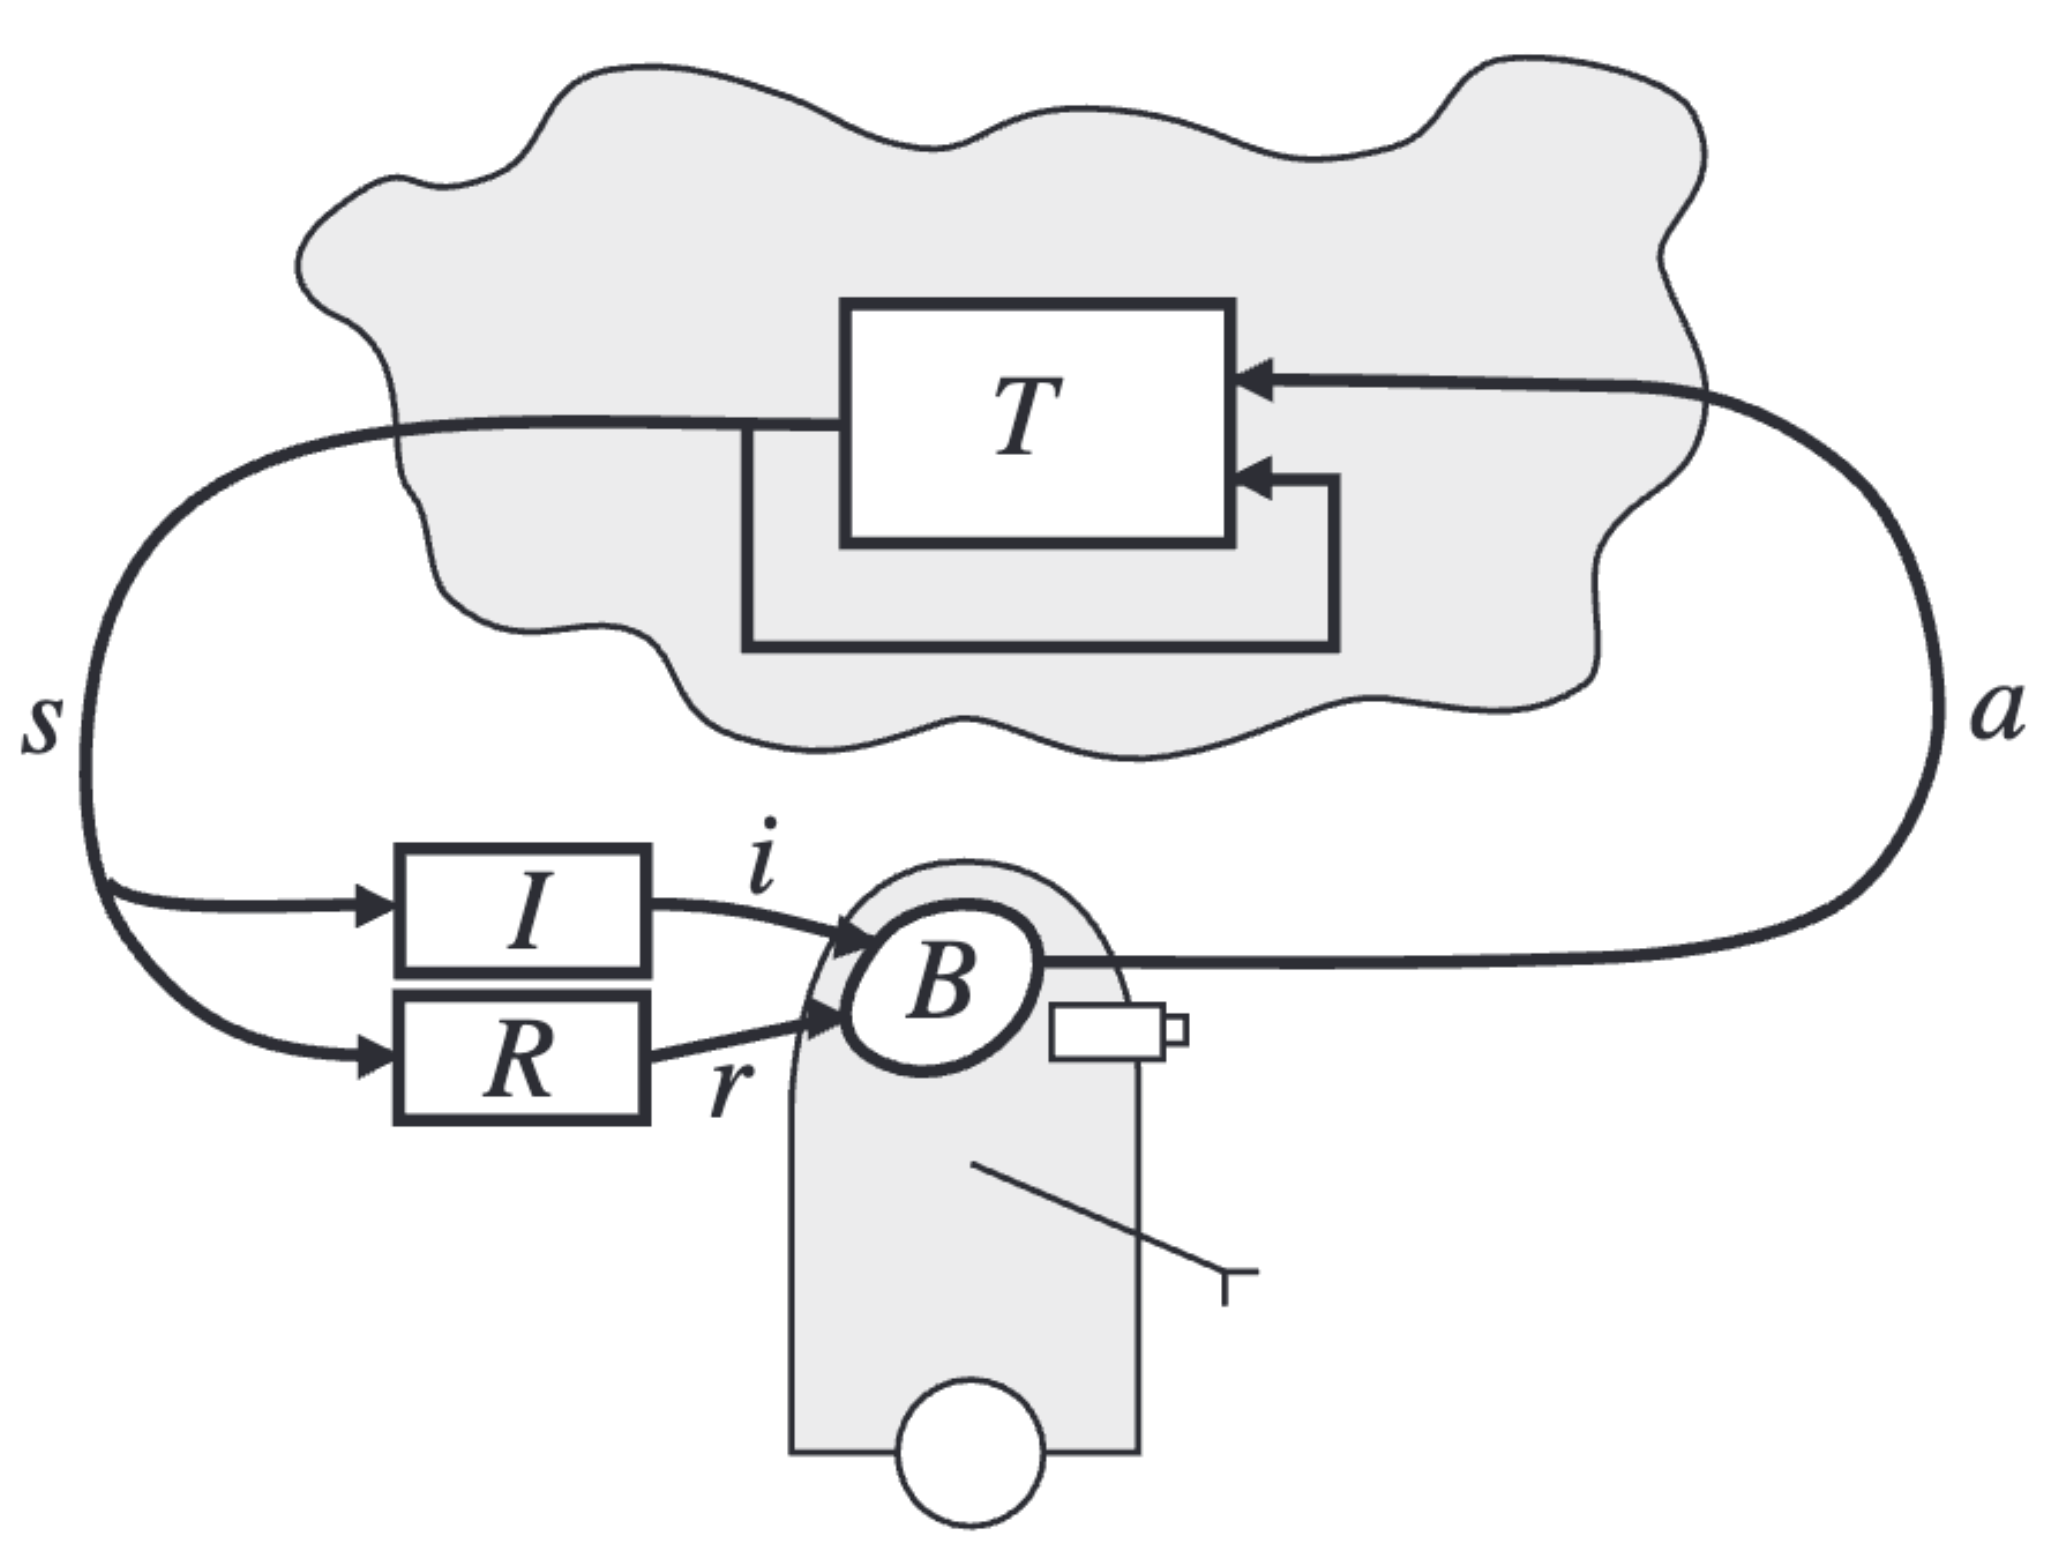
\includegraphics[width=10cm]{./imgs/RLGraph.png}
\caption{Reinforcement Learning Model Structure where $T$ is the environment, $B$ is the agent, $a$ is the action space and $s$ is the state space. The state space is then split into $I$ the observation space and $R$ the reward \cite{kaelbling1996reinforcement}}
\label{fig:RLGraph}
\end{figure}
\noindent
Using all of these concepts, reinforcement learning allows a learning process to occur by rewarding or punishing based on conditions outlined in the reward functions. Reinforcement learning therefore works on an iterative system where more time training will yield a better-performing neural network. This type of system can be seen in \autoref{fig:RLGraph} above.

\subsection{Reinforcement Learning Algorithms}
\subsubsection{Proximal Policy Optimization}
Proximal Policy Optimization \cite{SchulmanPPO} is a state-of-the-art reinforcement learning algorithm developed by OpenAi in 2017. ``Proximal policy optimization (PPO) is one of the most successful deep reinforcement learning methods, achieving state-of-the-art performance across a wide range of challenging tasks. However, its optimization behavior is still far from being fully understood'' \cite{Wang}. PPO combines ideas from both Advantage Actor Critic (A2C) and Trust region policy optimization (TRPO) \cite{SchulmanPPO}. The most important idea is that the policy should not change too much from the old policy.
\\\\
TRPO is a policy search method with monotonic improvement guarantee \cite{SchulmanTRPO}. In TRPO, the policy is iteratively updated by maximizing a surrogate objective over a trust-region around the most recent iterate policy $\pi_o_l_d$ \cite{Li}. A monotonic improvement guarantee is such that the algorithm will always improve or maintain the same performance. TRPO is often used in robotics and video game environments and is usually thought of as a more complex algorithm than PPO.
\\\\
A2C is an algorithm that takes ideas from policy-based and value-based algorithms. Policy-based algorithms will train an agent in order to come up with a policy that it expects to earn the maximum reward. Value-based algorithms train in order to estimate the value function to then guide the policy. This allows for A2C to be used in more environments. 
\\\\
Using elements from both A2C and TRPO, PPO algorithms ``are much simpler to implement, more general, and have better sample complexity (empirically)'' \cite{SchulmanPPO}. 

\subsubsection{Deep Q-Network}

Deep Q-Network is a reinforcement learning algorithm incorporating Q-learning and deep neural networks. The algorithm learns a Q function. A Q function or a value function is a function that will estimate the reward that an agent will receive if it chooses an action and continues to follow what it believes are optimal actions. The Q function is approximated using deep neural networks. The DQN algorithm, based on averaging previously learned Q-values estimates, which leads to a more stable training procedure and improved performance by reducing approximation error variance in the target values \cite{Anschel}.
\\\\
The DQN algorithm is used in many different areas, but it is most prominent in video games. Video games are such a good environment as DQN is very good at finding a policy that usually would not be clear \cite{mnih2013playing}. It also benefits from having strict and robust reward functions as they get rewarded at the end of a sequence of events, which robotics environments usually have. The DQN algorithm suffers from the disadvantages of slow convergence and excessive randomness during training \cite{YangMulti}. This will cause higher training time and can reduce the stability compared to other algorithms. 
\subsection{Problem}

This project intends to solve the problem of creating a simulator of the EE303 Mobile Robotics environment using OpenAI Gym \cite{brockman2016openai}, a reinforcement learning toolkit. The simulator will be designed to demonstrate how reinforcement learning can be used to solve problems traditionally using human-generated systems. The simulator should be able to train a model to follow a track with complex radii and intersections.
\\\\
The project has three main objectives:

\begin{enumerate}
  \item Develop a simulator for a differential drive line following robot using OpenAI Gym and other Python libraries. The simulator will account for all environmental factors that affect the EE303 Mobile robotics hardware. 

  \item Train a neural network using state-of-the-art reinforcement learning algorithms such as Proximal Policy Optimization and Deep Q-Network. The neural network should be able to follow the track's complex radii precisely.
  \item Port the trained model to the MSP432 of the robot. Debug and perform integration to solve all of the issues that arise. The ported model will then be analysed to see its performance.

\end{enumerate}

\subsection{Related Work}
This section aims to delve into all the different projects that relate to the problem at hand. Many different projects have used OpenAI Gym, PyGame and PyBullet to develop simulators for games and robotics. Through the study of these projects, it is possible to understand how elements can benefit this project.
\\\\
The work that I will be looking at in this section is the following: 
\begin{enumerate}
  \item Gym Hero: A Research Environment for Reinforcement Learning Agents in Rhythm Games 

  \item Reinforcement Learning and Adversarial Attacks on Player Model with Doodle Jump
  \item Panda-gym: Open-source goal-conditioned environments for robotic learning

  \item Car Racing

\end{enumerate}


\subsubsection{Gym Hero}
\\\\
Gym Hero is an environment developed in order to train an agent to play Guitar Hero, a rhythm game. A rhythm game is a subgenre of action games that challenges the player to follow a rhythm \cite{Adams} while pressing buttons on a controller or performing movements in front of motion detection devices \cite{GymHero}. In order to successfully play Guitar Hero, the player would press the button as it is displayed on the screen. Each button corresponds to a particular note in a song and must be pressed in sync with the music and the displayed graphically. 
\\\\
The environment called ``Gym Hero was developed using Python and PyGame graphics engine. It is divided into four parts: Notes and Buttons, Song, Score, and Game Loop'' \cite{GymHero}. Each of these different elements was created in graphics and in the back end where the logic was developed. The graphics were designed to be as simple as possible while being as close to Guitar Heros graphics. ``PyGame has a Sprite Group tool that allows calling the Draw and Update functions associated with each Sprite member of the Group'' \cite{GymHero}. The environment can be seen below in \autoref{fig:GymHero} to further understand the layout of the game. 
\\\\
\begin{figure}[H]
\centering
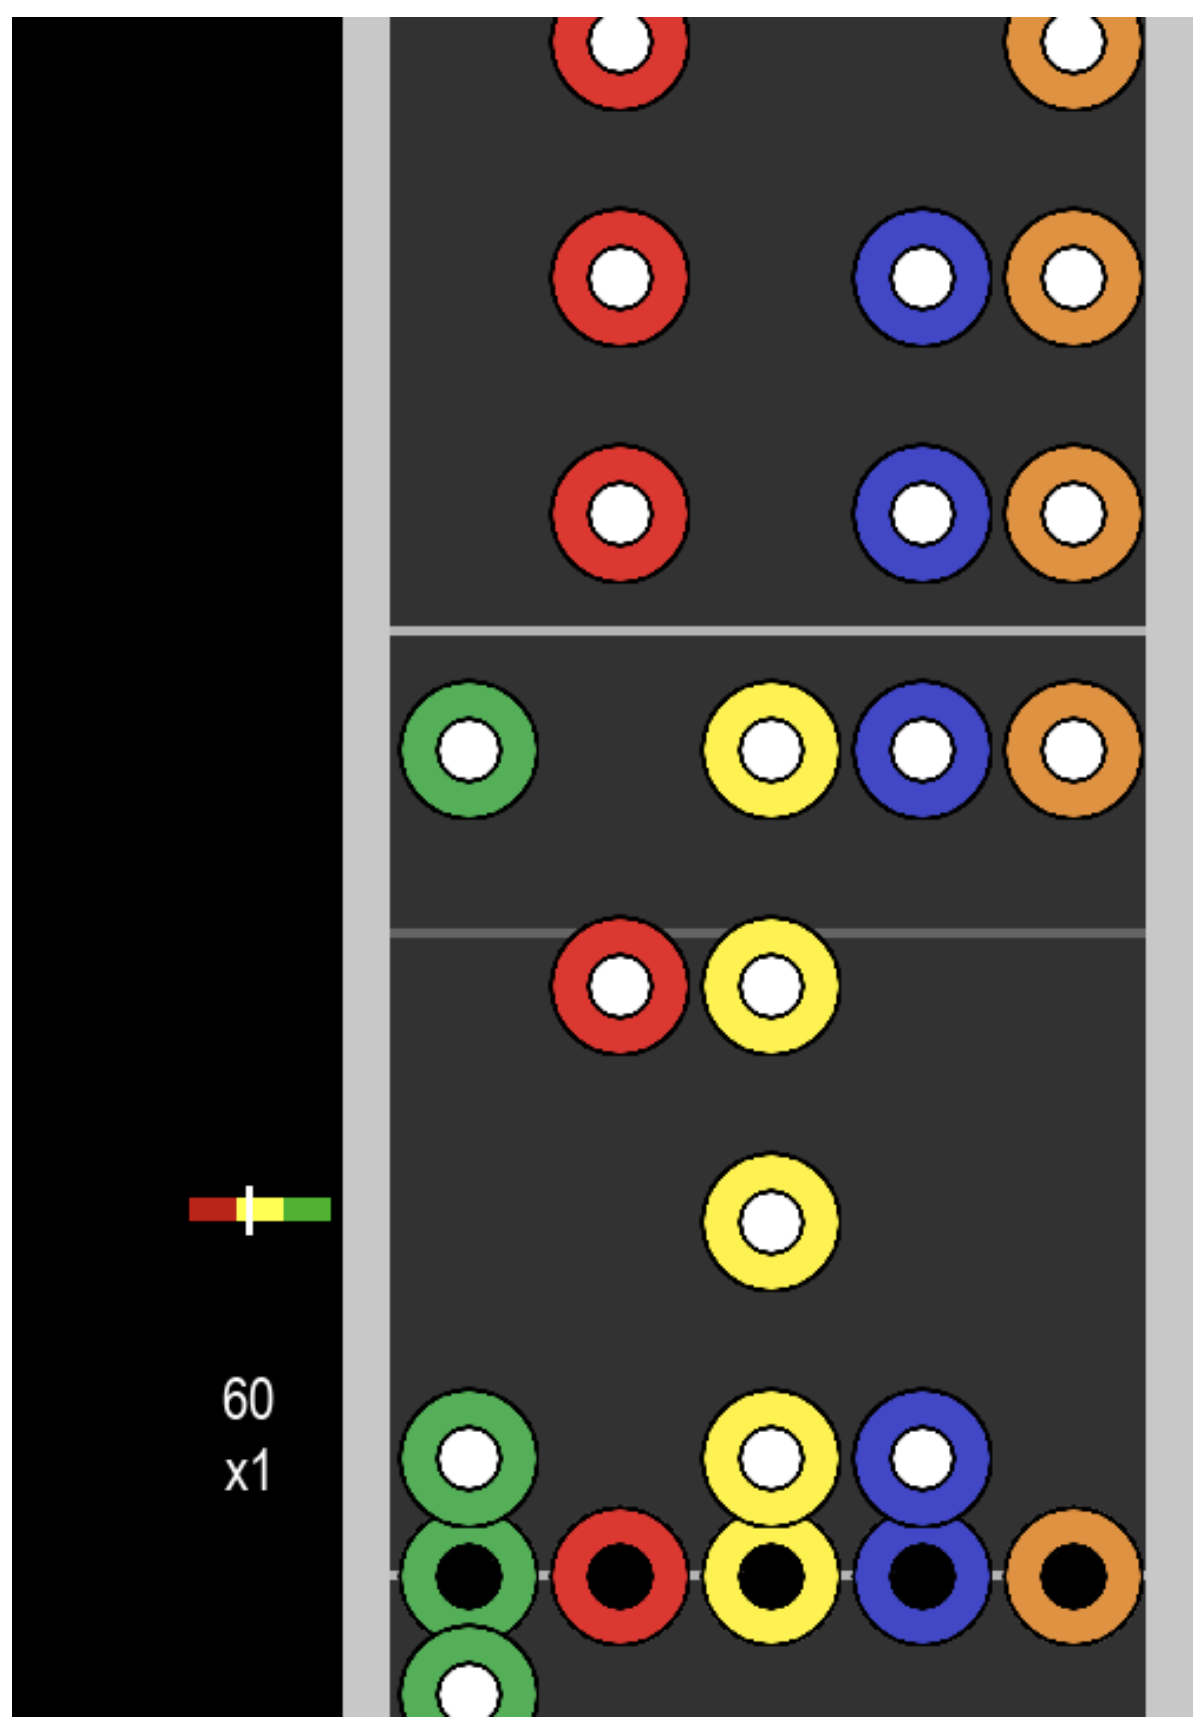
\includegraphics[width=8cm]{imgs/GymHero.png}
\caption{Gym Hero's user interface. Created to mimic the UI of Guitar Hero \cite{GymHero}.}
\label{fig:GymHero}
\end{figure}
\noindent
Gym Hero's use of observation, action and reward space is critical to analyse. The observation space used is a matrix containing an image of 500 pixels by 700 pixels. This uses just visual data to give the agent all its information; no supplementary information is provided. The action space used in the project is a discrete action space containing three to five actions depending on the difficulty level. Finally, the reward function is fairly straightforward, using three different scenarios. If the action results in a button hit, the agent will be rewarded. If the action results in a  button miss, then the agent will be punished. If the action results in no change to the environment's state, then no punishment or reward will be given. These spaces can be seen in Table \ref{tab:Gym Hero Observation Space}, \ref{tab:Gym Hero Action Space} and \ref{tab:Gym Hero Reward Space} below.
\\\\
\begin{table}[H]
\centering
\caption{Gym Hero Observation Space}
\label{tab:Gym Hero Observation Space}
\begin{tabular}{|ll|}
\hline
\textbf{Data Type} & \textbf{Description}\\ \hline
Matrix & Image Data from environment size 500$\times$700 pixels\\ \hline
\end{tabular}
\end{table}

\begin{table}[H]
\centering
\caption{Gym Hero Action Space (Difficult)}
\label{tab:Gym Hero Action Space}
\begin{tabular}{|ll|}
\hline
\textbf{Action} & \textbf{Description}\\ \hline
1 & Button one \\ \hline
2 & Button two \\ \hline
3 & Button three \\ \hline
4 & Button four \\ \hline
5 & Button five \\ \hline
\end{tabular}
\end{table}

\begin{table}[H]
\centering
\caption{Gym Hero Reward Space}
\label{tab:Gym Hero Reward Space}
\begin{tabular}{|ll|}
\hline
\textbf{Reward} & \textbf{Description}\\ \hline
+10 & Button hit \\ \hline
-10 & Button miss \\ \hline
0 & No change in state \\ \hline
\end{tabular}
\end{table}
\noindent
Gym Hero has many elements that are very applicable to this project. Using sprites for the graphics allows for easier movement and turning of images within PyGame. The reward function gives insight into how to structure a successful reward function; keeping it simple can be beneficial. 
\\\\
\subsubsection{Doodle Jump}
\\\\
Reinforcement Learning and Adversarial Attacks on Player Model with Doodle Jump aims to create an environment and train an agent to play the famous mobile game Doodle Jump. ``The main aim of the game is to propel `The Doodler’, the main character of the game which is a four-legged creature, up a never-ending series of platforms, without falling from them. The left end of the playing field connects to the right end to help the doodler stay within the bounds of the screen. The doodler can get a boost in score and height from springs attached to some platforms. There are monsters on some platforms that the doodler must avoid otherwise it will get killed on contact with the monster. The game ends when the doodler falls from a platform or when it hits a monster.''\cite{DoodleJump} The player will obtain more points as `The Doodler' gets higher. 
\\\\
Similarly to Gym Hero, PyGame is used to create the two-dimensional graphics for the game's environment. The graphics include the player, obstacles and monsters. Each of these incorporates its own collision detection to allow the player to jump and for monsters to kill the player. The graphics can be seen in \autoref{fig:DoodleJump} below to give a better impression of the game. 
\\\\
\begin{figure}[H]
\centering
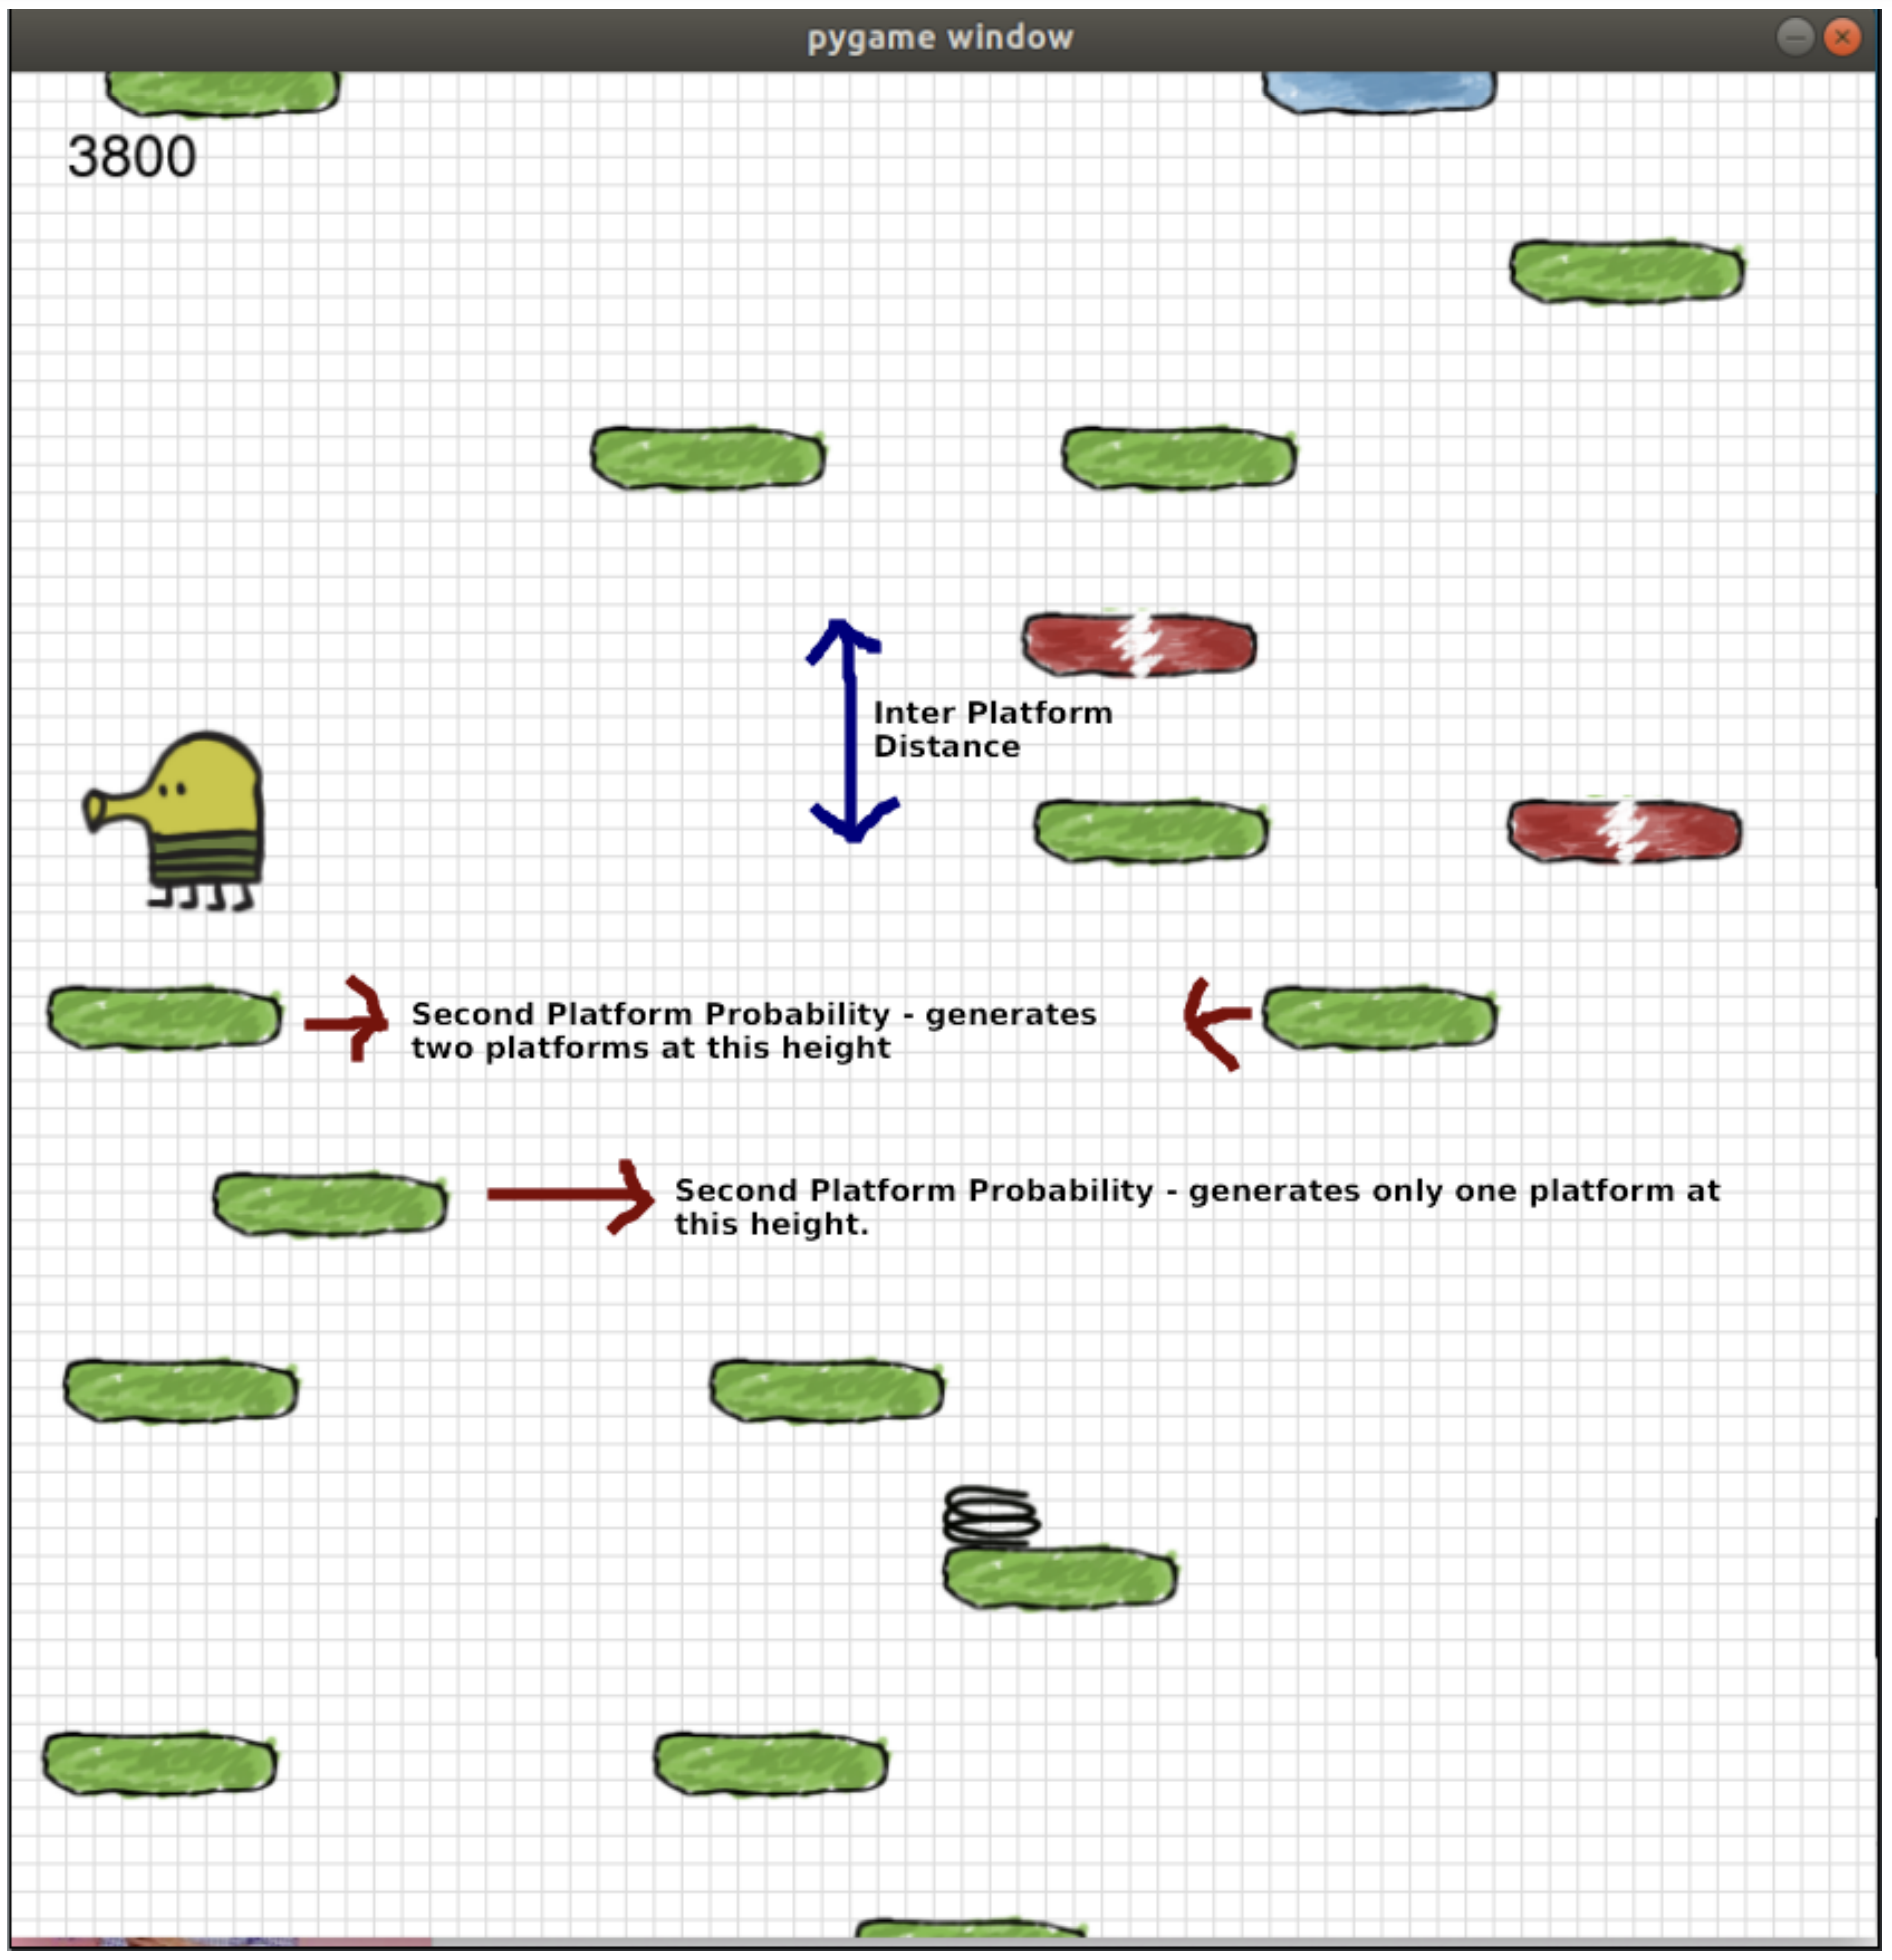
\includegraphics[width=8cm]{imgs/DoodleJump.png}
\caption{Doodle Jumps graphics including player,all platforms and obstacles \cite{DoodleJump}.}
\label{fig:DoodleJump}
\end{figure}\\\\
\noindent
The Doodle Jump environment uses different observation, action and reward spaces. The observation space is similar to before using a matrix containing the image data, which is compressed to allow for faster training. It is compressed from $800\times800$ pixels to $80\times80$ pixels. The action space is discrete, with only three separate actions. No action where there will be no horizontal movement, left action, and right action. This matches the movement options in the real game, although the movement uses the tilt of a device which could also be demonstrated with a single continuous action. Lastly, the reward function changes throughout the report, which demonstrates the different effects that rewards can have. The best reward space rewards progress upward without punishing for staying on the same platform. It punishes when the agent dies and when it hits a monster. It also gets rewarded for staying alive for a longer period of time. These spaces can be seen in Table \ref{tab:Doodle Jump Observation Space}, \ref{tab:Doodle Jump Action Space} and \ref{tab:Doodle Jump Reward Space} below.
\\\\
\begin{table}[H]
\centering
\caption{Doodle Jump Observation Space}
\label{tab:Doodle Jump Observation Space}
\begin{tabular}{|ll|}
\hline
\textbf{Data Type} & \textbf{Description}\\ \hline
Matrix & Image Data from environment size 800x800 pixels\\ \hline
\end{tabular}
\end{table}

\begin{table}[H]
\centering
\caption{Doodle Jump Action Space}
\label{tab:Doodle Jump Action Space}
\begin{tabular}{|ll|}
\hline
\textbf{Action} & \textbf{Description}\\ \hline
1 & No action\\ 
2 & Move left \\ 
3 & Move right \\ \hline
\end{tabular}
\end{table}

\begin{table}[H]
\centering
\caption{Doodle Jump Reward Space}
\label{tab:Doodle Jump Reward Space}
\begin{tabular}{|ll|}
\hline
\textbf{Reward} & \textbf{Description}\\ \hline
+3 & Score increases \\ 
+3 & Touch a spring \\ 
-2 & Dies \\ 
-4 & Touched by monster \\ 
 Variable & Living Reward \\ \hline
\end{tabular}
\end{table}
\noindent
This project has many similar elements to the Gym Hero project from the same discrete action spaces and the use of images for the observation space. Further research into different reward spaces creates a clearer path on how to create an optimised reward function.
\\\\
\subsubsection{Panda Gym}
\\\\
Panda-gym: Open-source goal-conditioned environments for robotic learning is a set of environments that aim to complete five tasks. These ``five tasks are included: reach, push, slide, pick and place and stack'' \cite{PandaGym}. The environments presented consist of a Panda robotic arm from Franka Emika, already widely used in simulation as well as in real in many academic works. It has 7 degrees of freedom and a parallel finger gripper. The robot is simulated with the PyBullet physics engine, which has the advantage of being open-source and shows very good simulation performance \cite{PandaGym}. These five different environments can be seen in \autoref{fig:Panda} below. 
\\\\
\begin{figure}[H]
\label{fig:Panda}
\centering
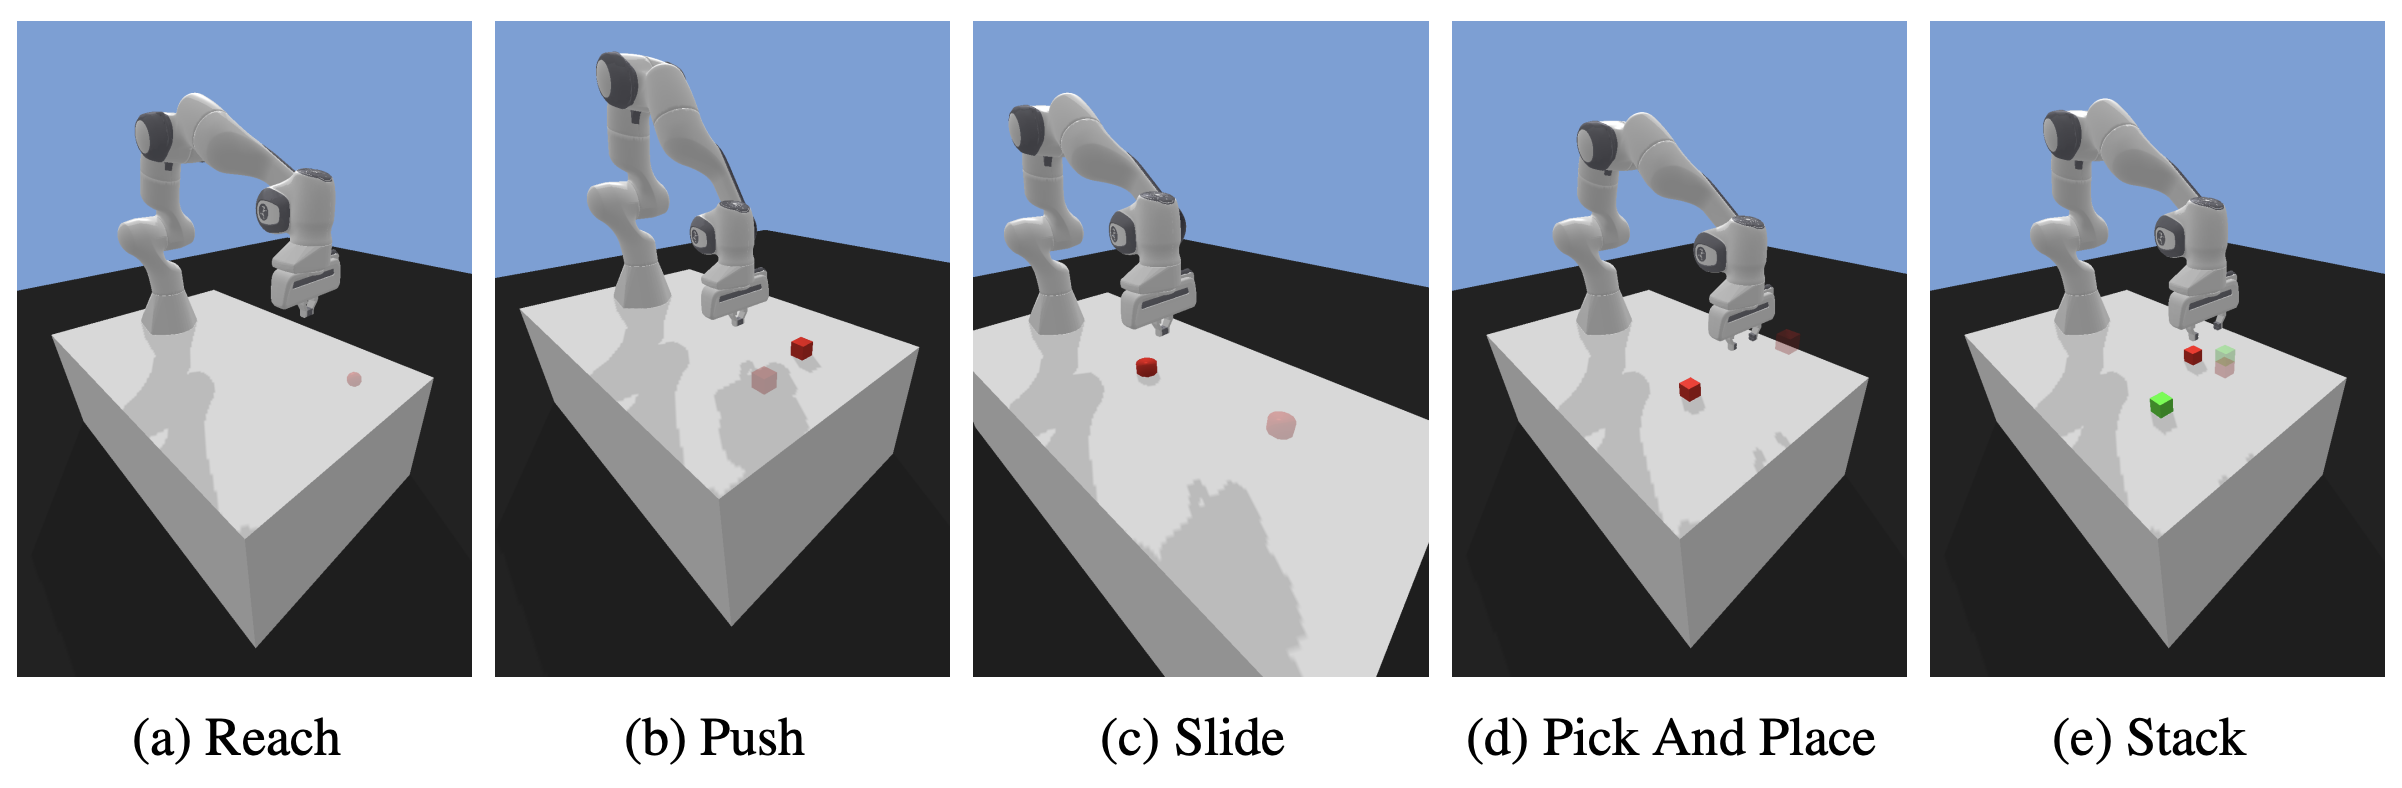
\includegraphics[width=15cm]{imgs/Panda.png}
\caption{All of the Panda environments for reinforcement learning. Robot has seven degrees of freedom.}
\label{fig:Panda}
\end{figure}\\\\
\noindent
Panda Gym uses PyBullet a three-dimensional physics engine, to simulate the rigid body robot. Through the use of URDF files and Robot Operating System PyBullet simulates all of the robot's degrees of freedom. The observation space has a different approach to the other projects, and it uses coordinates and speed. The coordinates would be the location of each of the joints, and the speed is the speed of the gripper. This is because, in a real world enviroment, each of these elements can be tracked without additional hardware. The action space is composed of the gripper movement command (3 coordinates, one for each axis of movement $x$, $y$ and $z$) and the fingers movement (1 coordinate, corresponding to the variation of the gripper opening). For some tasks, the gripper is closed. For these tasks, the action space is only composed of the gripper motion \cite{PandaGym}. The reward function is sparse and will reward with a value of 0 if the robot moves within 5cm of the target and will be punished otherwise. These spaces can be seen below in Table \ref{tab:Panda Gym Observation Space}, \ref{tab:Panda Gym Action Space} and \ref{tab:Panda Gym Reward Space}.
\\\\
\begin{table}[H]
\centering
\caption{Panda Gym Observation Space}
\label{tab:Panda Gym Observation Space}
\begin{tabular}{|ll|}
\hline
\textbf{Data Type} & \textbf{Description}\\ \hline
Coordinates & Joint positions (six coordinates) \\ \hline
\end{tabular}
\end{table}

\begin{table}[H]
\centering
\caption{Panda Gym Action Space}
\label{tab:Panda Gym Action Space}
\begin{tabular}{|ll|}
\hline
\textbf{Action} & \textbf{Description}\\ \hline
1 & X value (Continous)\\ 
2 & Y value (Continous)\\ 
3 & Z value (Continous)\\ 
4 & Finger coordinate (Continous)\\ \hline
\end{tabular}
\end{table}

\begin{table}[H]
\centering
\caption{Panda Gym Reward Space}
\label{tab:Panda Gym Reward Space}
\begin{tabular}{|ll|}
\hline
\textbf{Reward} & \textbf{Description}\\ \hline
0 & Within 5cm of target position\\ \
-1 & Not within 5cm of target position \\ \hline
\end{tabular}
\end{table}
\noindent
Panda Gym shows how to approach my problem from a more robotic view. In robotics, it is usually essential to use a physics engine for simulation, as there are countless forces on the robot. The use of coordinates and the robot's speed shows how a robot's observation space can be produced. The sparse reward function demonstrates that simpler reward functions might be easier to implement effectively.

\subsubsection{Car Racing}
The car racing project by Oleg Klimov is a car racing around a random track. The environment is created in PyGame, implementing a randomised track and a robot object. The environment is a bird's eye view of a racing track with a car. The robot will stay static on the screen, and the track will rotate and progress depending on the player's actions. An image of the environment can be seen below in \autoref{fig:CarRacing}.
\\\\
\begin{figure}[H]
\centering
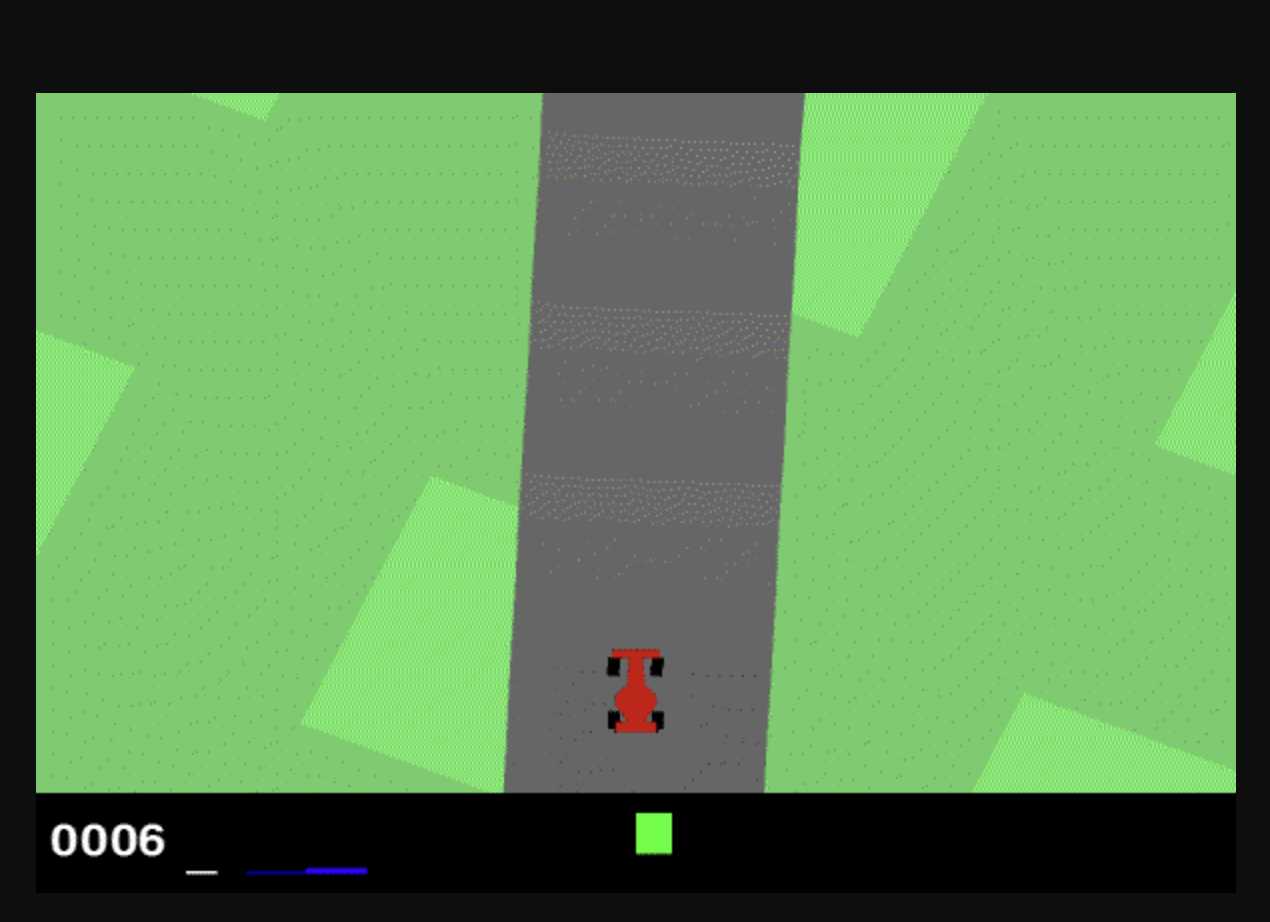
\includegraphics[width=10cm]{imgs/CarRacing.png}
\caption{The graphics of the car racing environment including the car and the randomised track \cite{Klimov}.}
\label{fig:CarRacing}
\end{figure}
\noindent
The environment for the car racing simulator uses a similar style of observation space as the Doodle jump and the Gym Hero spaces. The observation space is another matrix this time, it is a $96\times96$ pixel image. The action space can be both continuous and discrete in nature. ``If continuous: There are 3 actions: steering (-1 is full left, +1 is full right), gas, and breaking. If discrete: There are 5 actions: do nothing, steer left, steer right, gas, brake'' \cite{Klimov}. Finally the reward space is unique as it is trying to reward the speed of completion. The reward is -0.1 every frame and +1000/N for every track tile visited, where $N$ is the total number of tiles visited in the track. For example, if you have finished in 732 frames, your reward is $1000 - 0.1\times732 = 926.8$ points \cite{Klimov}. All of the spaces can be seen below in Table \ref{tab:Car Racing Observation Space}, \ref{tab:Car Racing Action Space (Continous)}, \ref{tab:Car Racing Action Space (Discrete)} and \ref{tab:Car Racing Reward Space}.
\\\\
\begin{table}[H]
\centering
\caption{Car Racing Observation Space}
\label{tab:Car Racing Observation Space}
\begin{tabular}{|ll|}
\hline
\textbf{Data Type} & \textbf{Description}\\ \hline
Matrix & Image Data from environment size 96x96 pixels\\ \hline
\end{tabular}
\end{table}

\begin{table}[H]
\centering
\caption{Car Racing Action Space (Continous)}
\label{tab:Car Racing Action Space (Continous)}
\begin{tabular}{|ll|}
\hline
\textbf{Action} & \textbf{Description}\\ \hline
1 & Steering (Continous)\\ 
2 & Gas (Continous)\\ 
3 & Breaking (Continous)\\ \hline
\end{tabular}

\end{table}
\begin{table}[H]
\centering
\caption{Car Racing Action Space (Discrete)}
\label{tab:Car Racing Action Space (Discrete)}
\begin{tabular}{|ll|}
\hline
\textbf{Action} & \textbf{Description}\\ \hline
1 & Steer left \\ 
2 & Steer right \\ 
3 & Gas \\ 
4 & Breaking \\ \hline
\end{tabular}
\end{table}

\begin{table}[H]
\centering
\caption{Car Racing Reward Space}
\label{tab:Car Racing Reward Space}
\begin{tabular}{|ll|}
\hline
\textbf{Reward} & \textbf{Description}\\ \hline
0 & Within 5cm of target position\\ 
-1 & Not within 5cm of target position \\ \hline
\end{tabular}
\end{table}
\noindent
The car racing environment explores elements of completion speed. This is beneficial to my problem as the faster the robot can follow the line, the more efficient it is performing. Overall, the rest of the spaces and the environment reinforce different approaches and techniques. 

\subsubsection{Conclusion}
In conclusion, from looking at all of the above projects developed using OpenAI Gym, there are a lot of takeaways. Using both PyGame and PyBullet to create the graphical and physics side of the simulator can make the process easier and faster. Each of the observation spaces uses its own method, although by studying the Panda Gym, an insight into robot-specific observation spaces can be obtained. Finally, the reward space of the functions differs from situation to situation. The main conclusion regarding them is that starting with a simple reward function will reduce failure. 

\section{Design}

\subsection{Choosing Python Physics Engine}

A significant element of creating the simulator was what Python libraries to use to emulate the physics of the environment. A Python library is essential for a fast and well-designed environment with all the different physics and collision detection. There are two obvious choices PyBullet, a 3D physics engine, and PyGame, a 2D platform for game development. These Python libraries are commonly used alongside OpenAI Gym to create accurate and latent environments. In order to choose to decide which would be the best for this project, both must be analysed and compared with each other.

\subsection{PyBullet}

PyBullet is a real-time physics simulation library for Python. PyBullet is most commonly used for the simulation of robots with multiple joints and for humanoid robots that mimic the movement of humans. PyBullet uses Robot Operating System to describe a robot's structure and kinematics. Each robot will be created using a Unified Robot Description Format file (URDF). Within these files, all of a robot's dimensions, links, joints and collision hitboxes are described. PyBullet uses these robot files to simulate all external forces as well as the internal forces exerted by the robot, such as DC motors. Through the use of PyBullet, a complete three-dimensional view of the robot can be displayed. An example of this environment can be seen below in \autoref{fig:PyBullet}.

\begin{figure}[h]
\centering
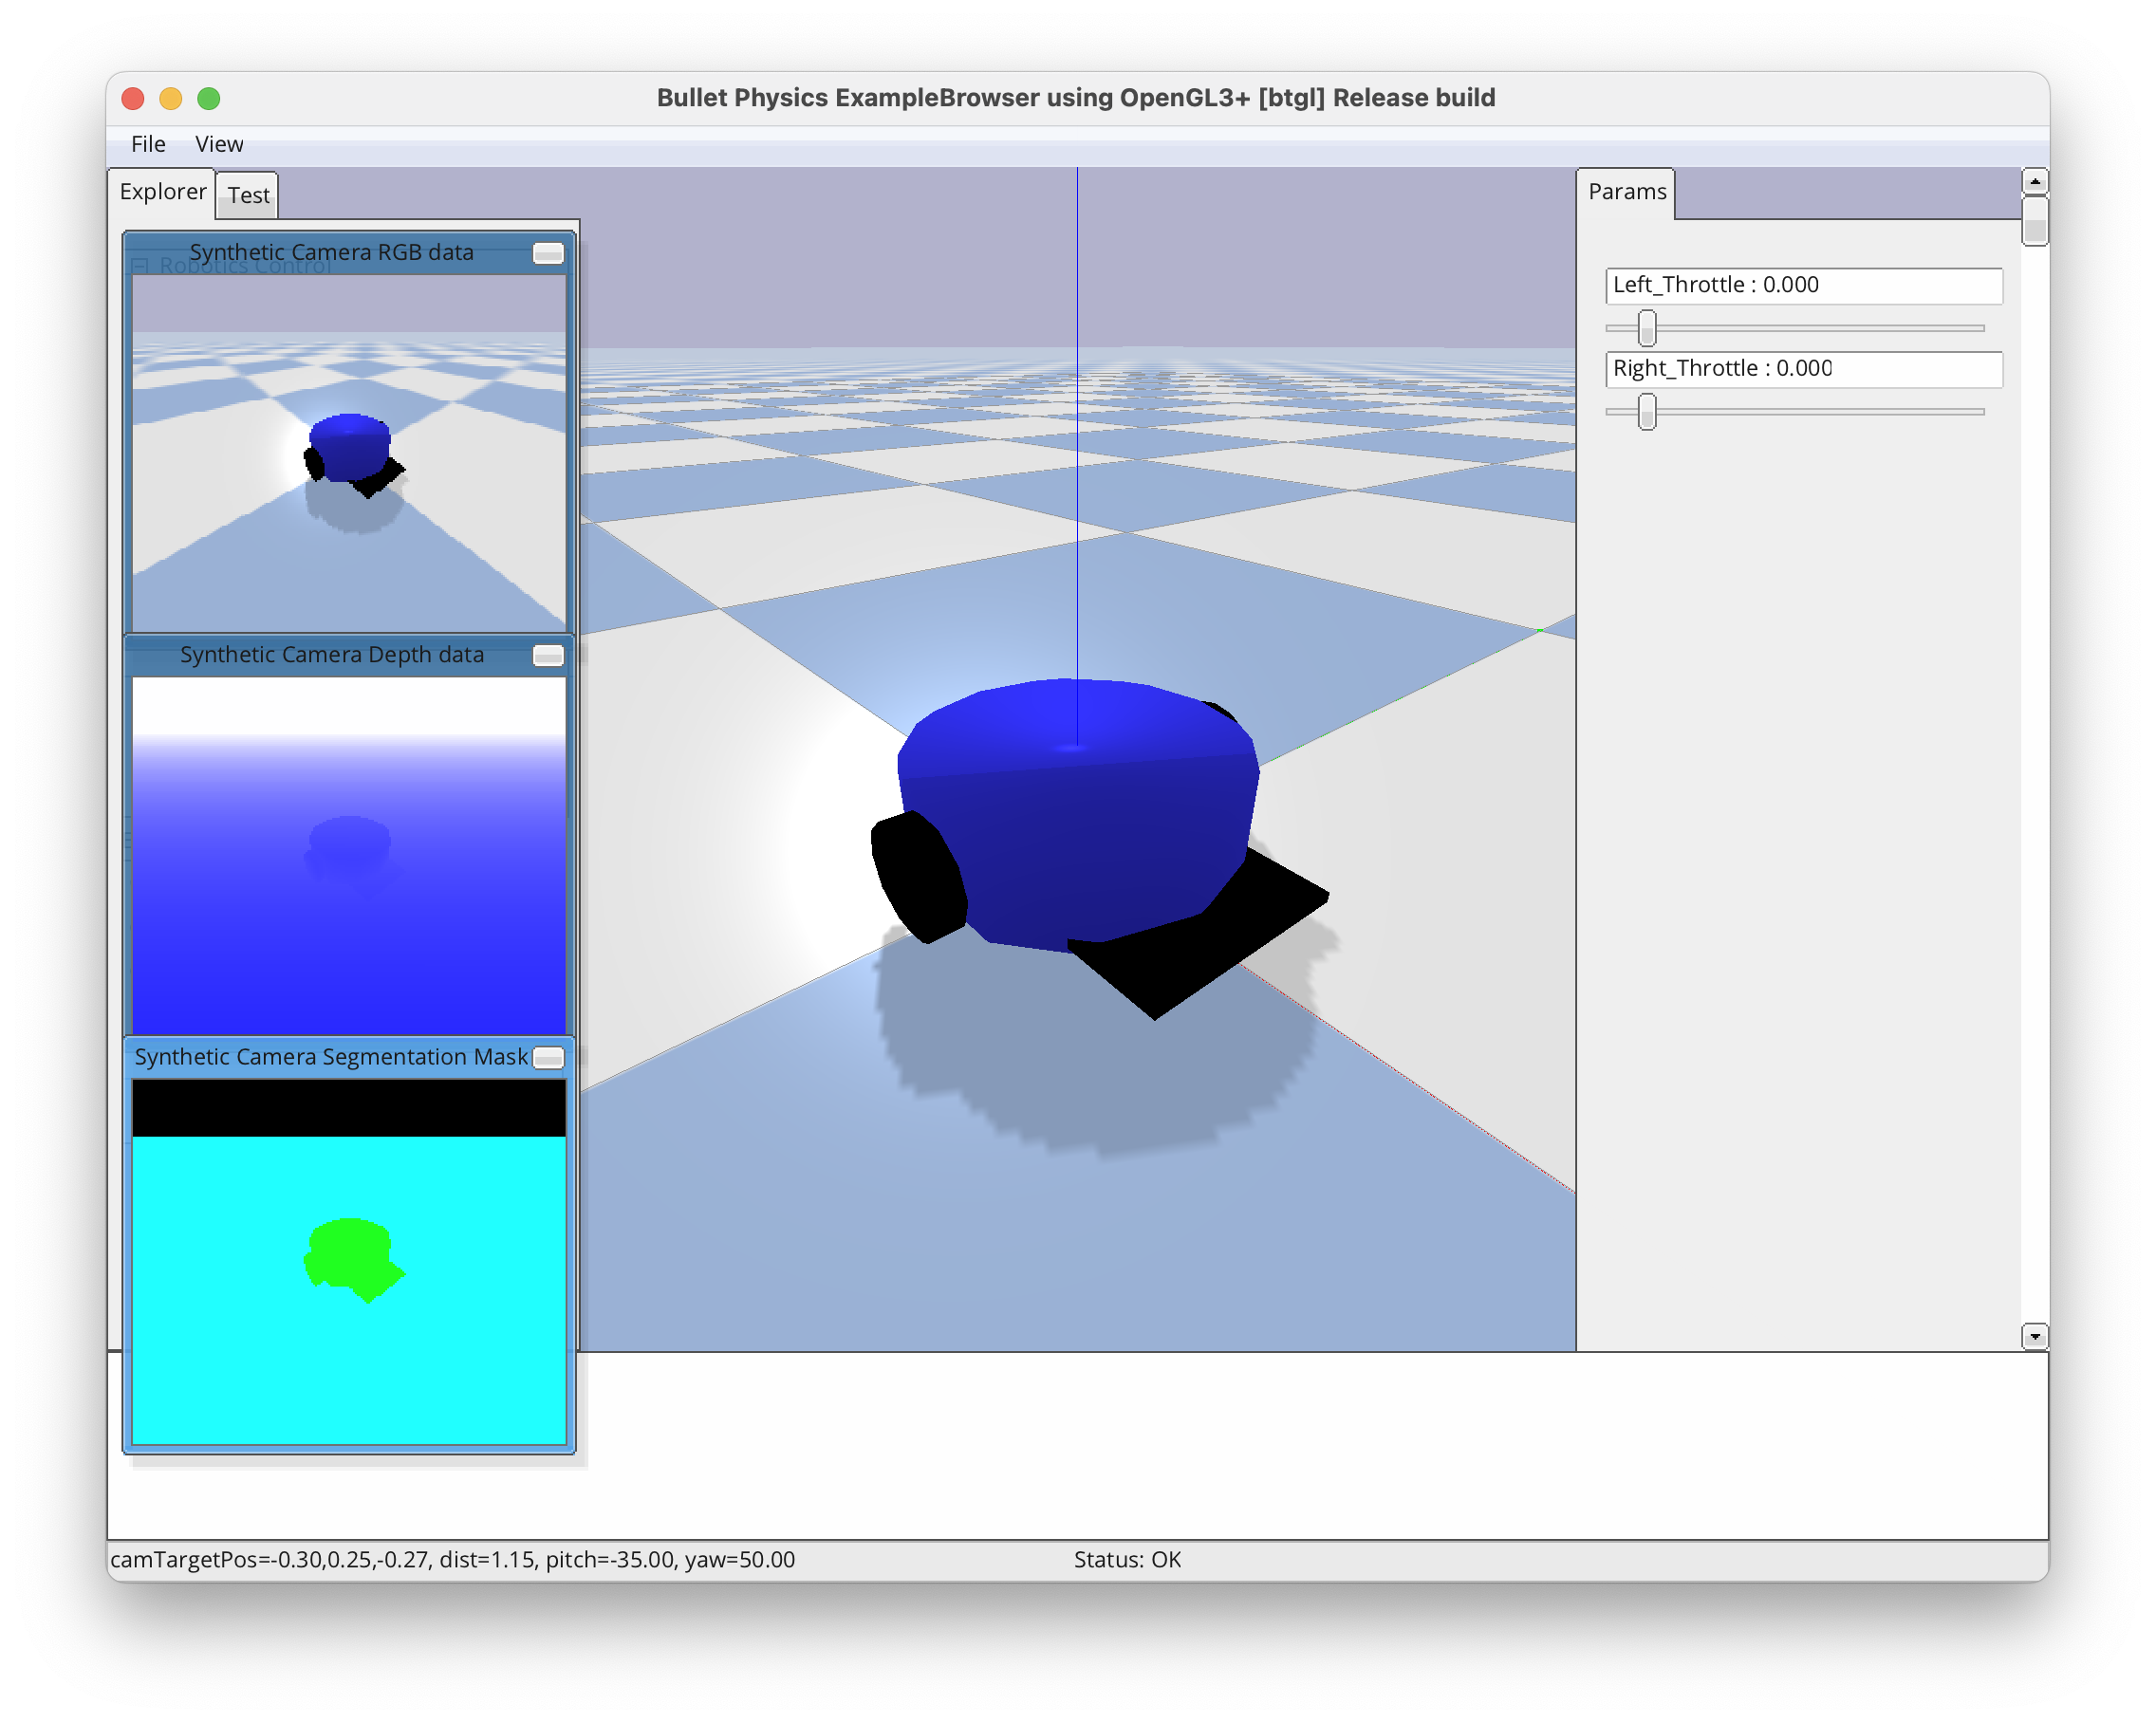
\includegraphics[width=12cm]{./imgs/PyBullet.png}
\caption{EE303's line follower robot simulated in a PyBullet environment}
\label{fig:PyBullet}
\end{figure}

\subsubsection{Advantages}

There are many different advantages of PyBullet, and these advantages include that PyBullet is a physics engine, PyBullet uses real-time rendering and PyBullet integrates with other libraries.

\begin{itemize}
  \item PyBullet can use the created URDF file to compute complex and very accurate physics about the robot and how it reacts in its environment. This allows all of the simulation's movement to be as close to real hardware as possible.

  \item PyBullet renders its graphics in real-time; this is very useful for debugging and visualising all of the movements and actions of the object.

\end{itemize}
% PyBullet is able to use the created URDF file to compute complex and very accurate physics about the robot and how it reacts in its environment. This allows for all of the movement in the simulation to be as close to real hardware as possible. 
% PyBullet renders its graphics in real time this is very useful for debugging and being able to visualize all of the movements and actions of the object.

\subsubsection{Disadvantages}

PyBullet's steep learning curve, hardware requirements, and community support are some of the disadvantages. 
\begin{itemize}
  \item PyBullet has a steep learning curve; to set up and get a basic robot moving is easy enough, but when more complex elements are being added, it becomes increasingly difficult for new users.
  \item As PyBullet is a complete physics engine, it requires a certain standard of hardware to run smoothly. In order to know what standard of hardware is needed to implement the simulator, the simulator must first be built. This adds a level of uncertainty to the final performance.
  \item PyBullet needs more community support; although it has many users, the resources available are limited, making this a significant disadvantage. 

\end{itemize}
 
\subsection{PyGame}

PyGame is a 2D game development platform for Python that allows for the user interface and other basic mechanics to be designed and implemented. PyGame is most commonly used by developers who are create low-computational 2D games. Unlike PyBullet PyGame does not use any URDF files. PyGame can use images as objects in the user interface (UI). 

\subsubsection{Advantages}
Some advantages of PyGame are its large community, in-depth documentation and low hardware requirements. 

\begin{itemize}
  \item PyGame compared to PyBullet has a massive community and very active community. This is a significant advantage as so many different projects can be studied to learn how to implement features. 
  \item In comparison to PyBullet PyGame is so much more accessible and easy to learn due to the in-depth documentation provided. It makes it more intuitive to implement. 

  \item As PyGame is a 2D environment, it allows for the computational load to be far lower. Along with the fact that the user is to design any of the physics, it gives full control of the computational requirement and allows for quick and latent programmes.


\end{itemize}


\subsubsection{Disadvantages}

Some disadvantages of PyGame are the following; physics must be designed, and its limited graphic capabilities. 
\begin{itemize}
  \item As PyGame does not have an in-built physics engine or logic, it leaves this for the programmer to develop. This increases the code that must be developed and increases the time needed. 
  \item The limited graphics capabilities are a disadvantage, as no animations, arent built in they must be developed by the user. These include some image rotations and movements and this can lead to complex solutions.

\end{itemize}


\subsection{Differential Drive Function}
As for my decision to use PyGame rather than PyBullet, no physics engine is built in. Therefore, creating a model for a differential drive line following robot is essential. The robot uses two DC motors, one on each side, along with a caster wheel to prevent dragging. The robot can be seen in \autoref{fig:RobotBottom} below.
\\\\
\begin{figure}[H]
\label{fig:1}{}
\centering
\includegraphics[width=8cm]{imgs/RobotBottom.png}
\caption{Image of the bottom of EE303's line following robot showing the two motors, caster wheel and sensor array}
\label{fig:RobotBottom}
\end{figure}
\noindent
Three main aspects need to be accounted for when dealing with a differential drive robot: the angle theta, the $x$ coordinates, and the $y$ coordinates. Using these three makes it possible to position the robot anywhere. The other two elements that dictate future positions are the two motor velocities.
\\\\
The equations for positioning can be seen below:


\begin{equation}
\begin{aligned}
X = X+((V_L+V_R)/2) \cos\theta \times T \\
Y=Y-((V_L+V_R)/2) \sin\theta \times T \\
\theta=\theta+(V_L-V_R)/W \times T
\end{aligned}
\end{equation}\\
where $V_L$ is equal to the velocity of the left motor, $V_R$ is equal to the velocity of the right motor, $T$ is the time, $W$ is the width of the robot and $\theta$ is the angle of the robot\\\\
\begin{figure}[H]
\centering
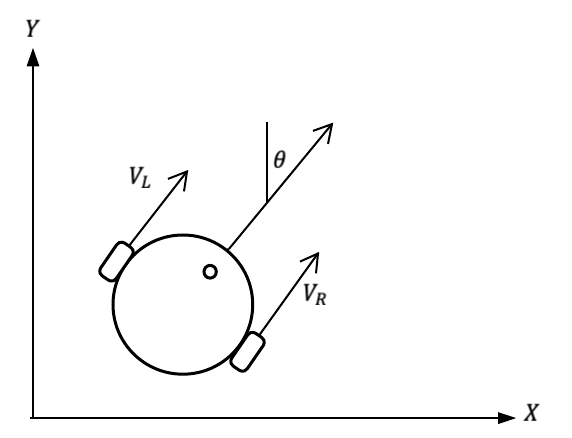
\includegraphics[width=10cm]{imgs/DiffGraph.png}
\centering
\caption{Diagram of the robot showing each of the variables that dictate the current and future locations}
\label{fig:DiffGraph}
\end{figure}
\noindent
Using these three equations above, and the diagram in \autoref{fig:DiffGraph}, the differential drive logic can be implemented. PyGame uses Sprites, images that can move around the user interface and interact with its surroundings. Using Sprites allows the use of transform functions necessary for this movement on the screen. Using PyGame's transform function, the robot can move around the UI.

\subsection{Collision Detection}
Collision detection checks two objects and can return if they have collided or intersected. Collision detection works by first getting the coordinates of two objects, and it compares this to check if their given width or height overlaps. If their dimensions overlap, a collision has occurred at some stage in the last time step.
\\\\
PyGame has two different methods of detecting collisions following the logic above. The first and most basic method uses horizontal and vertical conditions to detect collisions. The algorithm will check whether object $B$'s edges are within $A$'s vertical edges. If this is the case, the same will be checked in the horizontal direction. A collision has occurred if both are true. A diagram in \autoref{fig:RectCollision} demonstrates this type of collision.

 \begin{figure}[H]
 \centering
 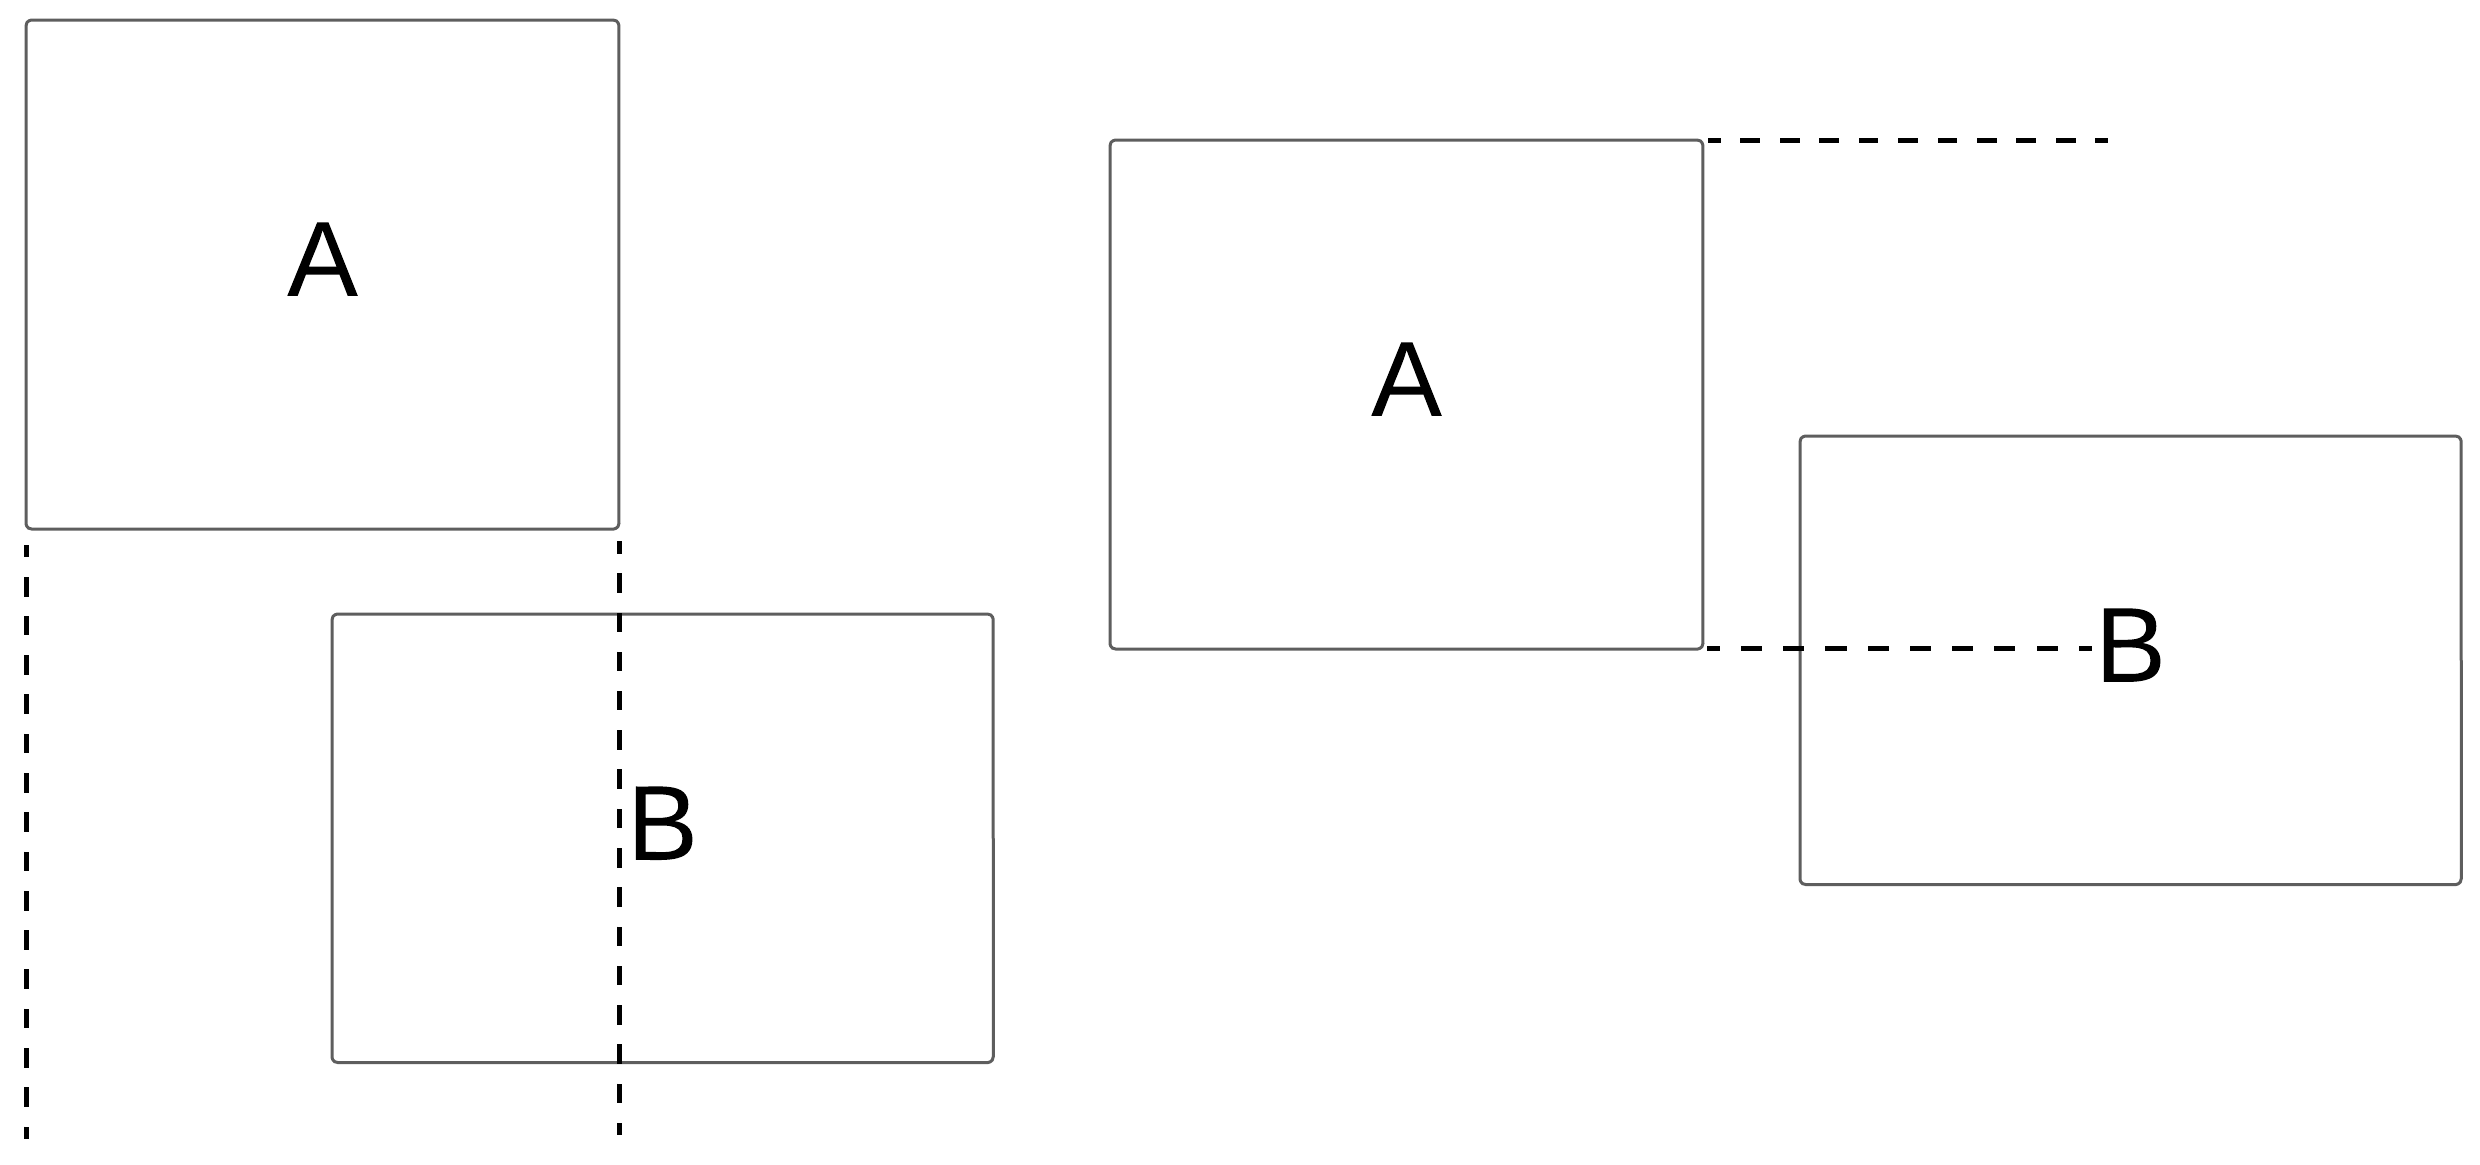
\includegraphics[width=10cm]{imgs/RectCollision.png}
 \caption{Diagram to show how Pygame detects collisions using an image's vertical and horizontal edges}
 \label{fig:RectCollision}
 \end{figure}
\noindent
The second method of collision detection is pixel-perfect collision detection. This method uses Python's built-in mask feature. Masks take an image and then classify the image pixel by pixel. If the pixel is blank, then it will be set as false or otherwise true. This will make an image more defined than an image’s rectangular shape. This can be seen in \autoref{fig:MasksCollision} below. Once both objects have masks, each pixel can be compared to see if they are equal. If this is the case, then a collision has occurred.


 \begin{figure}[H]
 \centering
 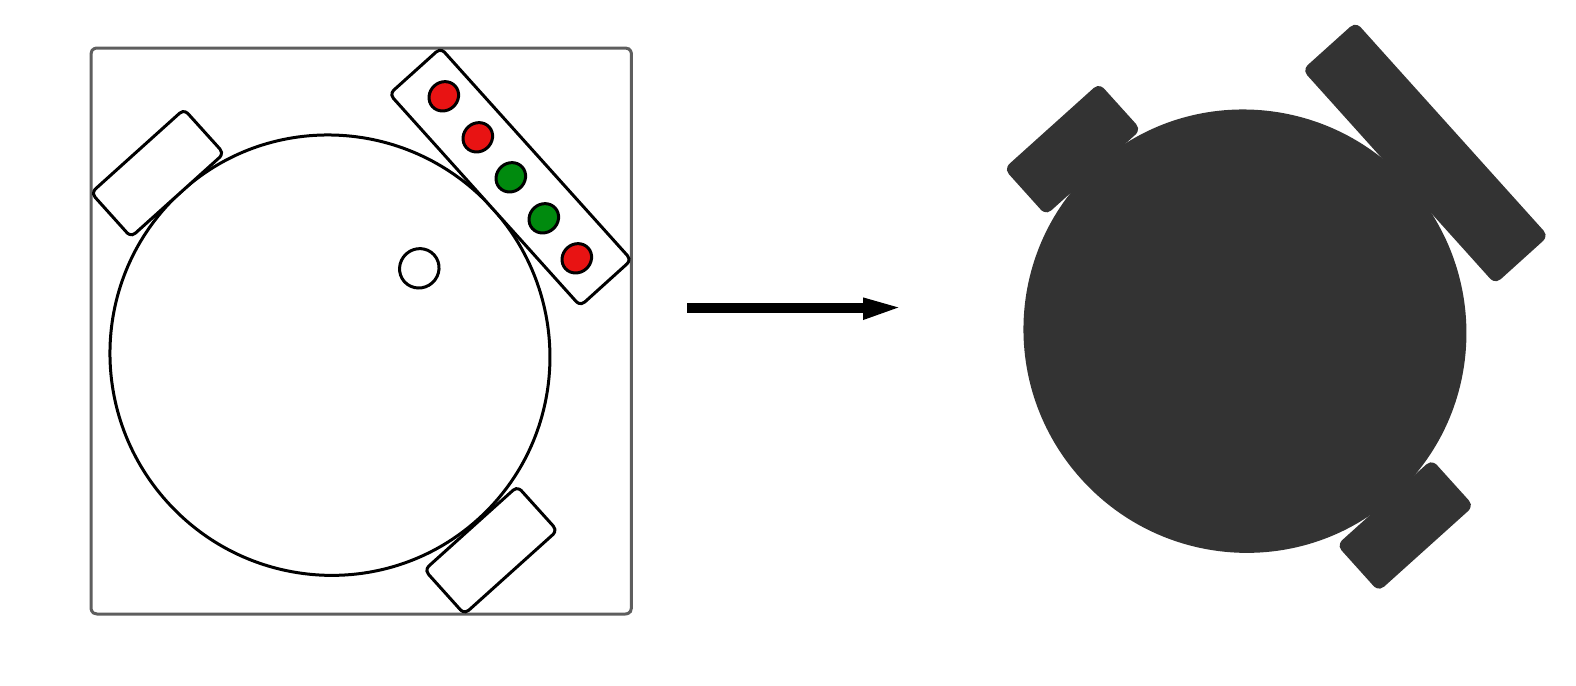
\includegraphics[width=10cm]{imgs/MasksCollision.png}
 \caption{Diagram showing how a rectangular image can be converted into a mask for pixel-perfect collision detection}
 \label{fig:MasksCollision}
 \end{figure}
 \noindent
In the simulator's design, I opted to use the pixel-perfect collision detection for the following reasons. Firstly, line detection accuracy is an essential part of the simulator, so pixel-perfect detection was needed. As I had planned to stop training as soon as the robot was no longer on the line, this was the logical decision. Secondly, as the track is so complex in its design, the most straightforward and intuitive method to use is to convert the image of the track to a mask rather than generating a whole track design. This track can be seen in \autoref{fig:Track} below.


 \begin{figure}[H]
 \centering
 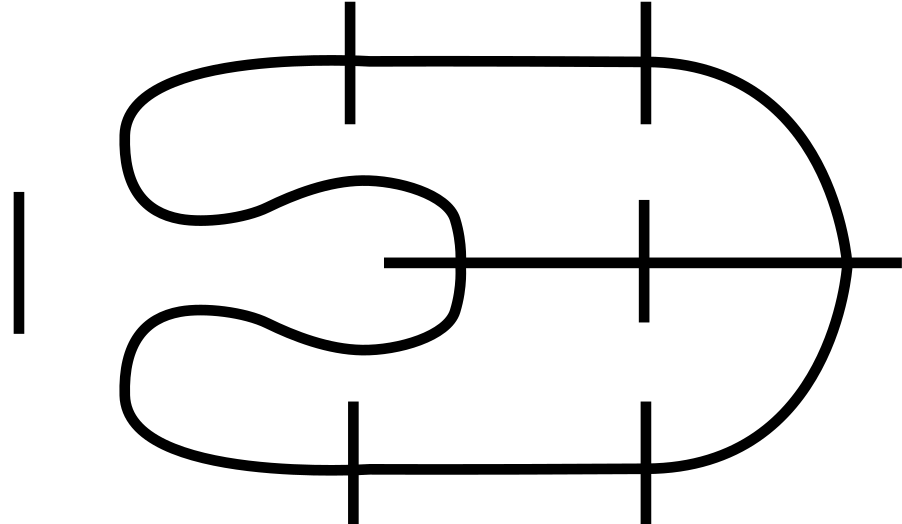
\includegraphics[width=10cm]{imgs/Track.png}
 \caption{EE303's track showing all of the complex radii and intersections \cite{KevinMcGuinness}}
 \label{fig:Track}
 \end{figure}

\subsection{Action Space}
The action space is all of the different effective options the agent can take \cite{zhu2021overview}. Action spaces are broken down into two distinct sections continuous and discrete. Discrete action spaces are usually more straightforward than continuous action spaces. Both of these action spaces were developed for the environment. 

\subsubsection{Discrete Action Space}
Discrete action spaces contain only discrete actions that have been predefined. These could include arrow key presses within video games. This use of predefined actions limits the agent to a very specific type and amount of actions. This can help in the early stage of training an agent as it makes debugging easier and can have lower training times.
\\\\
The discrete action space that was developed included only four discrete actions: Forward and stopped for each of the motors. The use of only four actions allowed the agent to train quickly. The reward function reduces the number of states that can occur. This is because the state where both motors are stopped is not possible as the training will be terminated. 

\subsubsection{Continous Action Space}
Continuous action spaces allow for infinite actions to be used, although they are bounded between two values. This allows for more fine control of actions compared to discrete action spaces. This will allow for smoother performance in robotics, although it might result in lengthier training times. Continuous action spaces are usually used in more complex problems such as robotics. 
\\\\
The continuous action space was developed using a similar range of values. The action space was bounded between zero and one, and this gives infinite actions. The agent can vary the speed of the motors from stopped to full speed. 

\subsection{Observation Space}
The observation space is all the information the agent has to make its next action. Some common data include coordinates, velocity, sensor values, number of objects, etc. Changing the observation space can have a significant impact on its training. If too much data is provided, it will only make training slower, and too little data will reduce the model's performance. \autoref{fig:ObservationSpace} below shows the circular nature of the observation space about its environment, agent, reward and action space.

\begin{figure}[H]
\centering
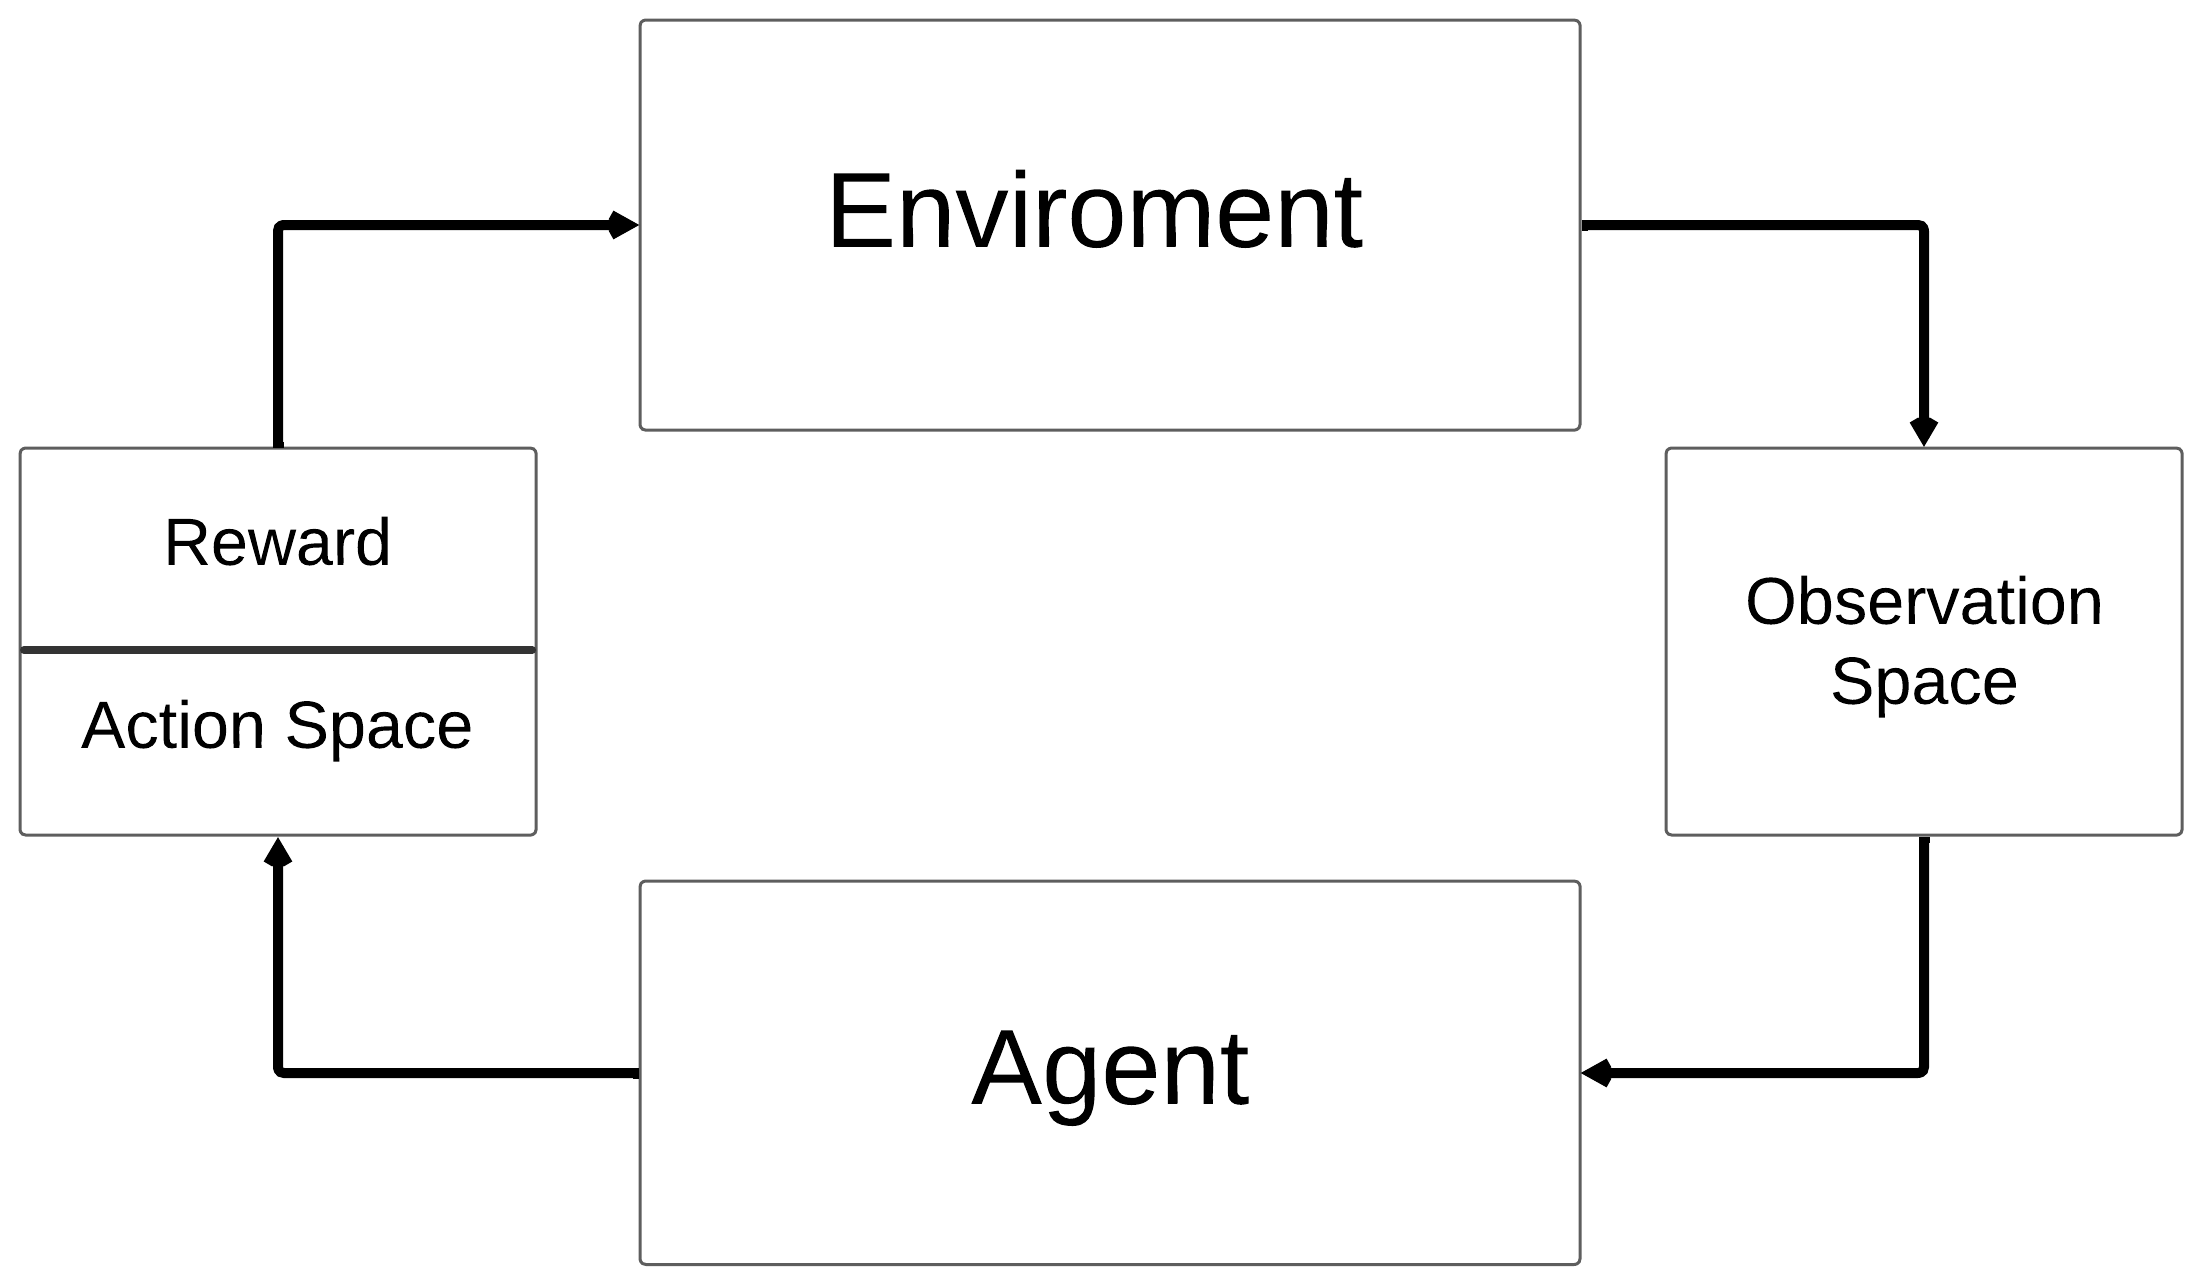
\includegraphics[width=7cm]{imgs/ObservationSpace.png}
\caption{The circular nature of reinforcment learning. This shows how the agent uses its observation to make a decision and be rewarded}
\label{fig:ObservationSpace}
\end{figure}

 

\subsubsection{Initial Observation Space}

Initially, the observation space included the $x$ and $y$ coordinates, the velocity of each wheel, the angle of the robot and the five sensor values. Each of these elements gives the agent different information for its decision. The observation space can be seen in the \autoref{fig:InitialObsSpace} below.

\begin{figure}[H]
\centering
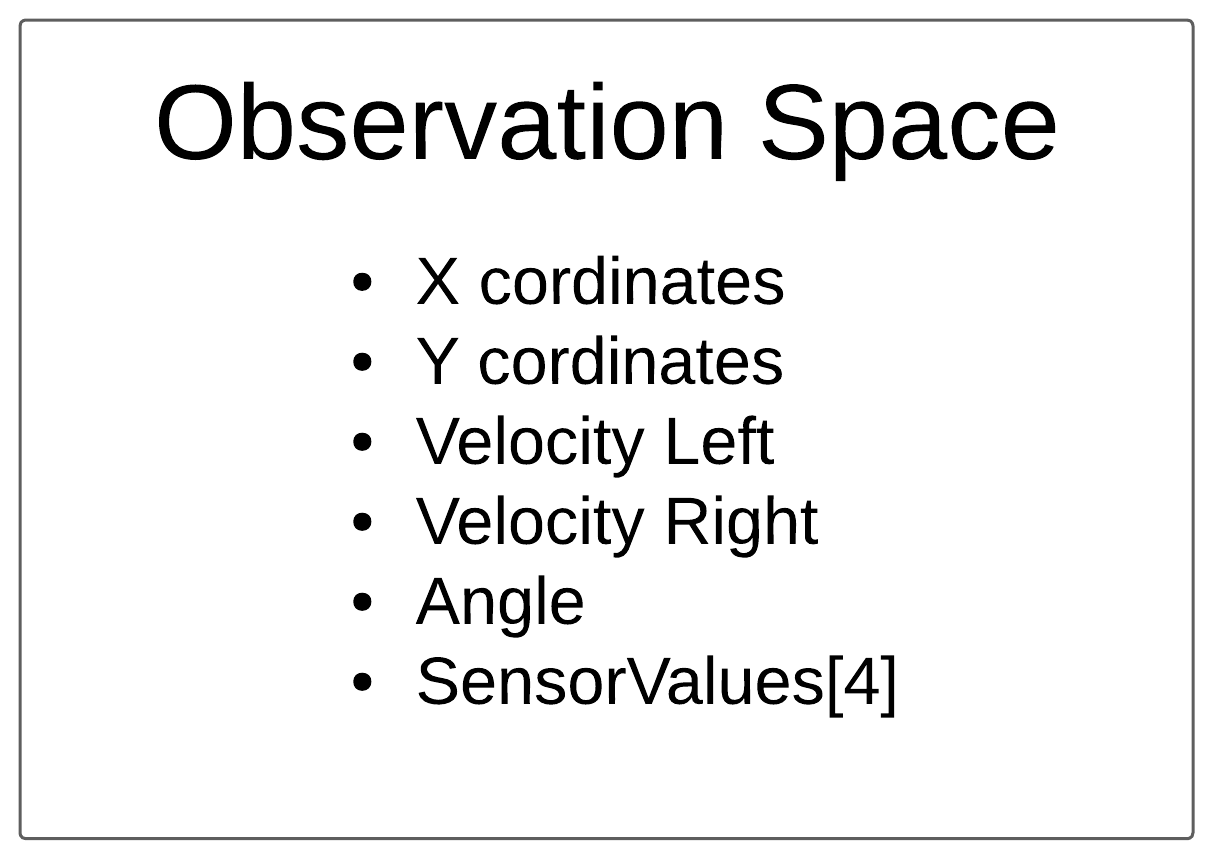
\includegraphics[width=7cm]{imgs/InitialObsSpace.png}
\caption{The initial observation space including the robot's position, orientation, velocity and present sensor values}
\label{fig:InitialObsSpace}
\end{figure}

 \noindent
After using this observation space for training, it was leading to poor results, and the rate at which it was learning was very low. This makes sense as it has too much data, and this leads to increased training time.
\\\\
With further thought, this observation space was incorrect for this simulator's goals. The observation space on the physical hardware would only be able to know its $x$ and $y$ coordinates or its angle if the robot uses DC motors with an encoder. With this in mind, it allows for changes in the observation space to be made.


\subsubsection{Simplified Observation Space}

To simplify the observation space, it can be reduced to just the sensor values. This is the most simplified version of an action space and the easiest to implement. The observation space can be seen in the \autoref{fig:SimpleObsSpace} below. 

\begin{figure}[H]
\centering
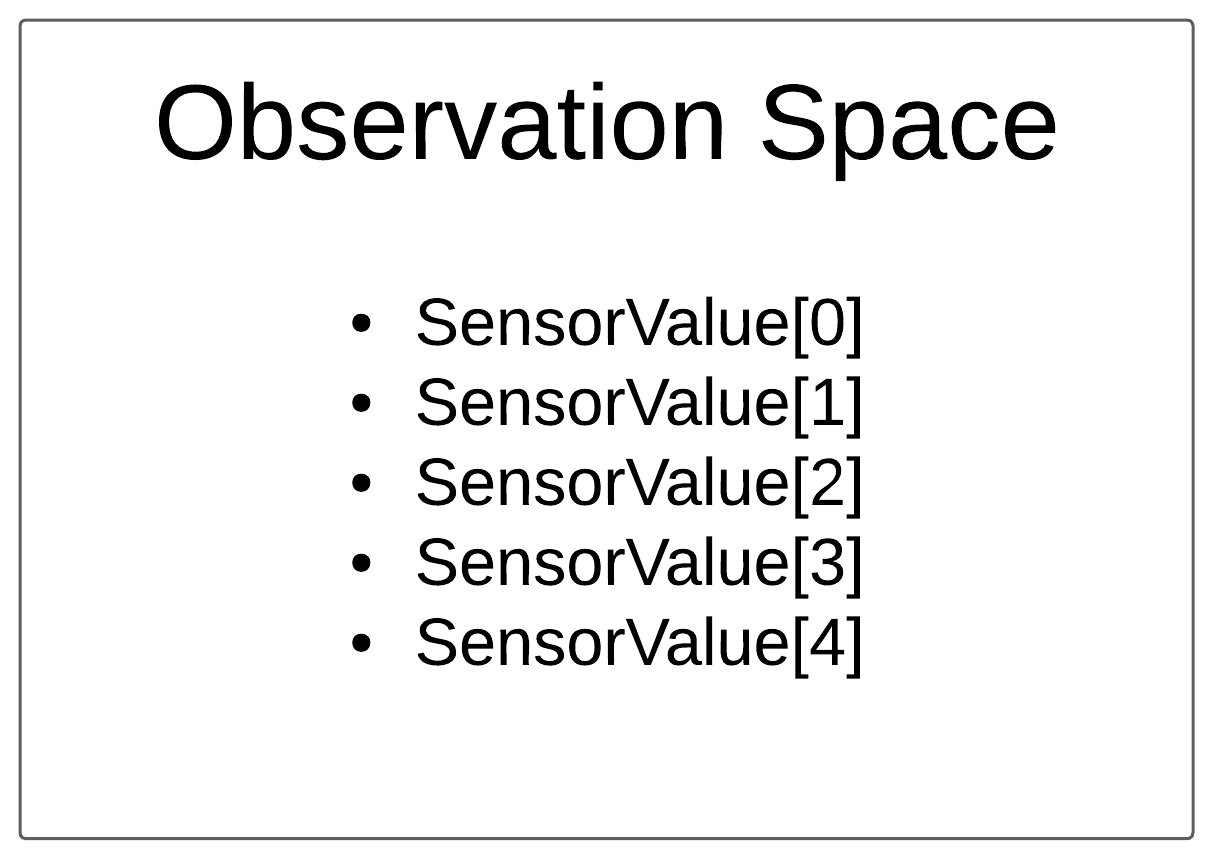
\includegraphics[width=7cm]{imgs/SimpleObsSpace.png}
\caption{A simplified observation space simplified down to just the current sensor values}
\label{fig:SimpleObsSpace}
\end{figure}
\noindent
After using this observation space for training, the agent struggled with the intersections on the EE303 track. It would view these intersections as turns, and then turn. In order to train this model, a more simplified track was used. This track removed the intersections so that the agent could only train on the complex radii. This simplified track can be seen below in \autoref{fig:SimpleTrack}. With this change, the trained model proved to be very effective.

\begin{figure}[H]
\centering
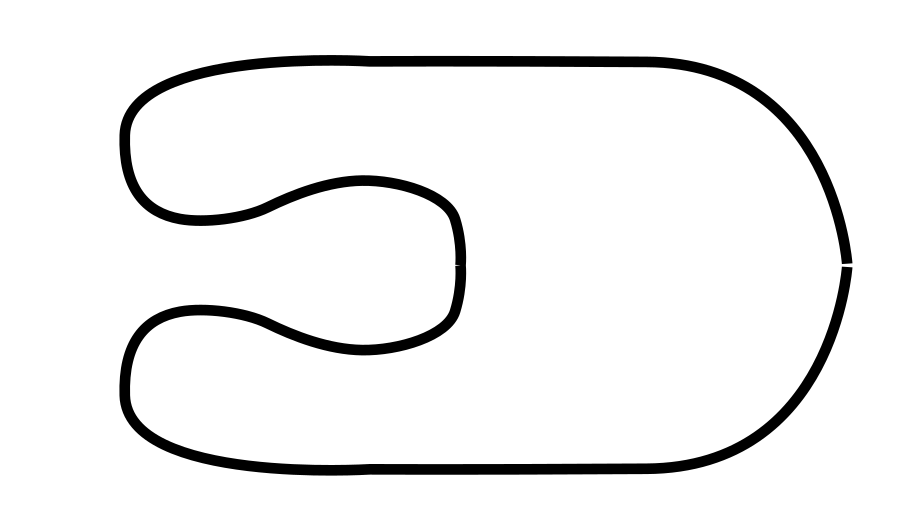
\includegraphics[width=10cm]{imgs/SimpleTrack.png}
\caption{Simplified version of EE303's track used to develop a working observation space \cite{KevinMcGuinness}}
\label{fig:SimpleTrack}
\end{figure}

 
\subsubsection{Final Observation Space}

The final observation space was inspired by the simplified observation space above, although it implements a history. The idea of the history is to give the agent more information on where the robot was in the past, enabling the robot to make a more informed decision. The observation space contains the current sensor values and the past five sensor values. This results in an array of size thirty. This observation space can be seen in \autoref{fig:FinalObsSpace} below.

\begin{figure}[H]
\centering
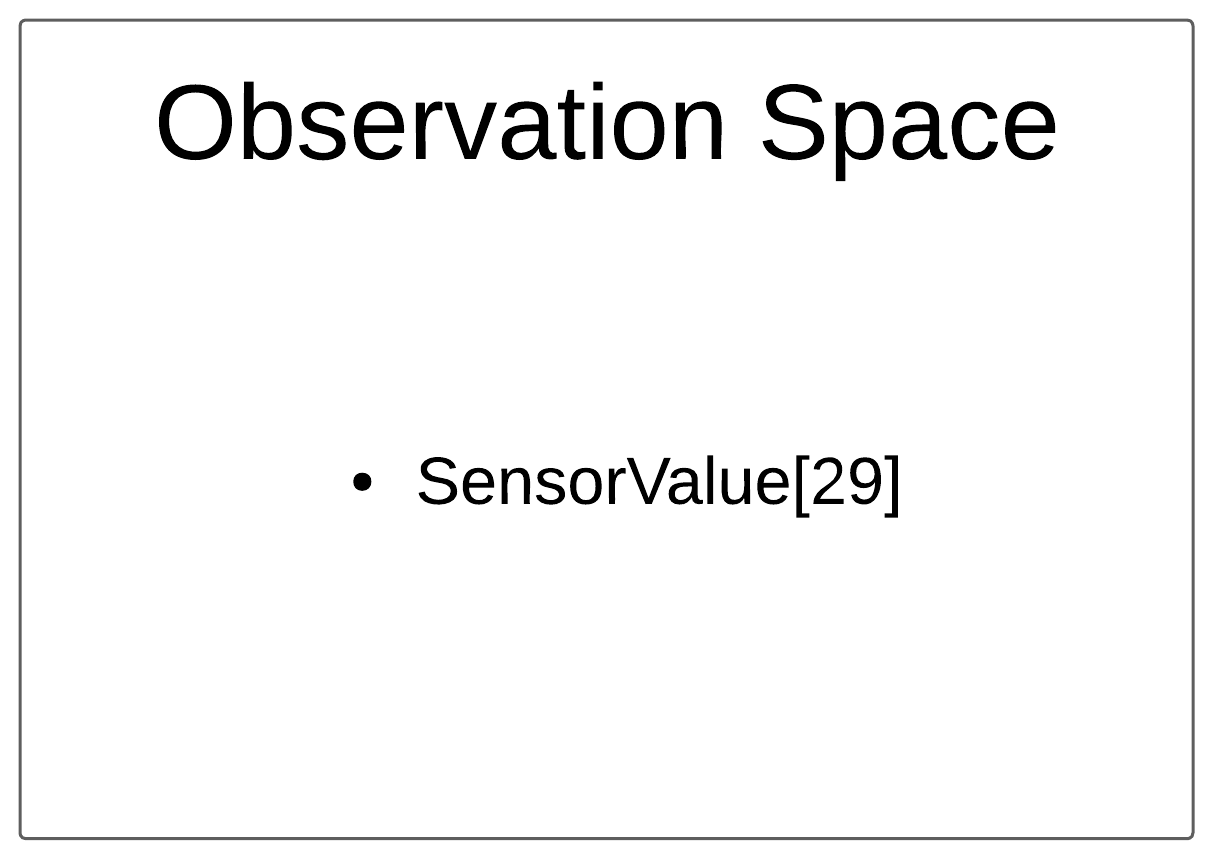
\includegraphics[width=7cm]{imgs/FinalObsSpace.png}
\caption{The final observation space including just thirty sensor values. One present set and five historic sets of values}
\label{fig:FinalObsSpace}
\end{figure}
\noindent 
This observation space was used to train the model with the simplified track. This showed an improvement in performance and in the time required to train to an adequate level. The initial track was then used to train and was able to navigate accurately and quickly.
 


\subsection{Reward Function}

The reward function is how the agent can know whether the actions taken are correct or if it has made a negative action. The reward function is what drives reinforcement learning and generally is similar to the problem description \cite{niekum2011evolution}. The reward is one of the most critical functions as it allows an agent to train efficiently or not at all. This must be defined correctly, as the agent can quickly find methods to maximise its reward without completing the objective.

\subsubsection{Initial Reward System}

Initially, the logic for the reward system was as follows, if the robot were on the line, it would be rewarded, and if the robot were off the line, it would be punished, and the training would reset and restart. This is because the robot is required to be on the line, and whenever it makes an action to leave the line, it should be punished. A snippet of the reward function can be seen in \autoref{fig:InitialCode} below.
\\\\

\begin{figure}[H]
\begin{lstlisting}[language=Python]
if(robot is on line)
  reward++
else
  reward--
  terminated = True
\end{lstlisting}
\caption{Pseudocode for Initial Reward System}
\label{fig:InitialCode}
\end{figure}
\noindent
This function is correct in its approach, although it does not account for the robot's velocity. The agent will quickly learn that there is no need to move as long as the robot is on the line as it will keep racking up the rewards.
 

\subsubsection{Further Reward System}

Building on the flaws of the initial reward system, an improved reward system can be created. The new logic is that when the robot is off the line, it will be punished, and the training terminated. The robot will be rewarded only when the robot is on the line and the sum of the velocity of the wheels is greater than zero. This should prevent the robot from staying still and promote movement. The code snippet can be seen below in \autoref{fig:FurtherCode}.
\\\\
\begin{figure}[H]
\begin{lstlisting}[language=Python]
if(robot is on line and velocities > 0)
  reward++
else
  reward--
  terminated = True
\end{lstlisting}
\caption{Pseudocode for Further Reward System}
\label{fig:FurtherCode}
\end{figure}
\noindent
This improves the initial reward system, and the robot will begin to move around the track. Again the agent exploits this logic quite quickly and learns that if the robot is to move backwards and forwards, it can maximise its rewards. It also learns that it does not always have to move. This logic needs the incentive to complete the track at a fast pace.


\subsubsection{Final Reward System} 

The final reward system takes elements from each iteration of the reward system before. It uses the following logic: when the robot is not on the line or not moving, the training will be terminated and restarted, if the robot is moving and on the line, it will be rewarded and, after a set amount of time, terminated and restarted. The time limit will enable the agent to improve and maximise its rewards within a fixed period rather than having an infinite amount of time and reward capability. The code snippet can be seen in \autoref{fig:FinalCode}.
\\\\
\begin{figure}[H]
\begin{lstlisting}[language=Python]
if(robot is on line and velocities > 0)
  reward++
else
  terminated = True
\end{lstlisting}
\caption{Pseudocode for Final Reward System}
\label{fig:FinalCode}
\end{figure}
\noindent
This reward function balances both the reward and the punishment. It performs well and allows the agent to improve on every iteration, preventing wasted time when the robot stops and allowing the robot to follow the line accurately and quickly.

\subsection{Choosing RL Algorithm}

\subsection{Training}
Once the environment has been created, training the neural net is possible. We can train the environment locally and on DCU's GPU server using the two reinforcement learning algorithms mentioned earlier, DQN and PPO. The environment developed can be seen in \autoref{fig:PyGame}. The training process will involve allowing the agent to run within the environment for many timesteps to learn iteratively. The training process can take hours to train a working model, and this would run the model through tens of millions of timesteps. 

\begin{figure}[H]
\centering
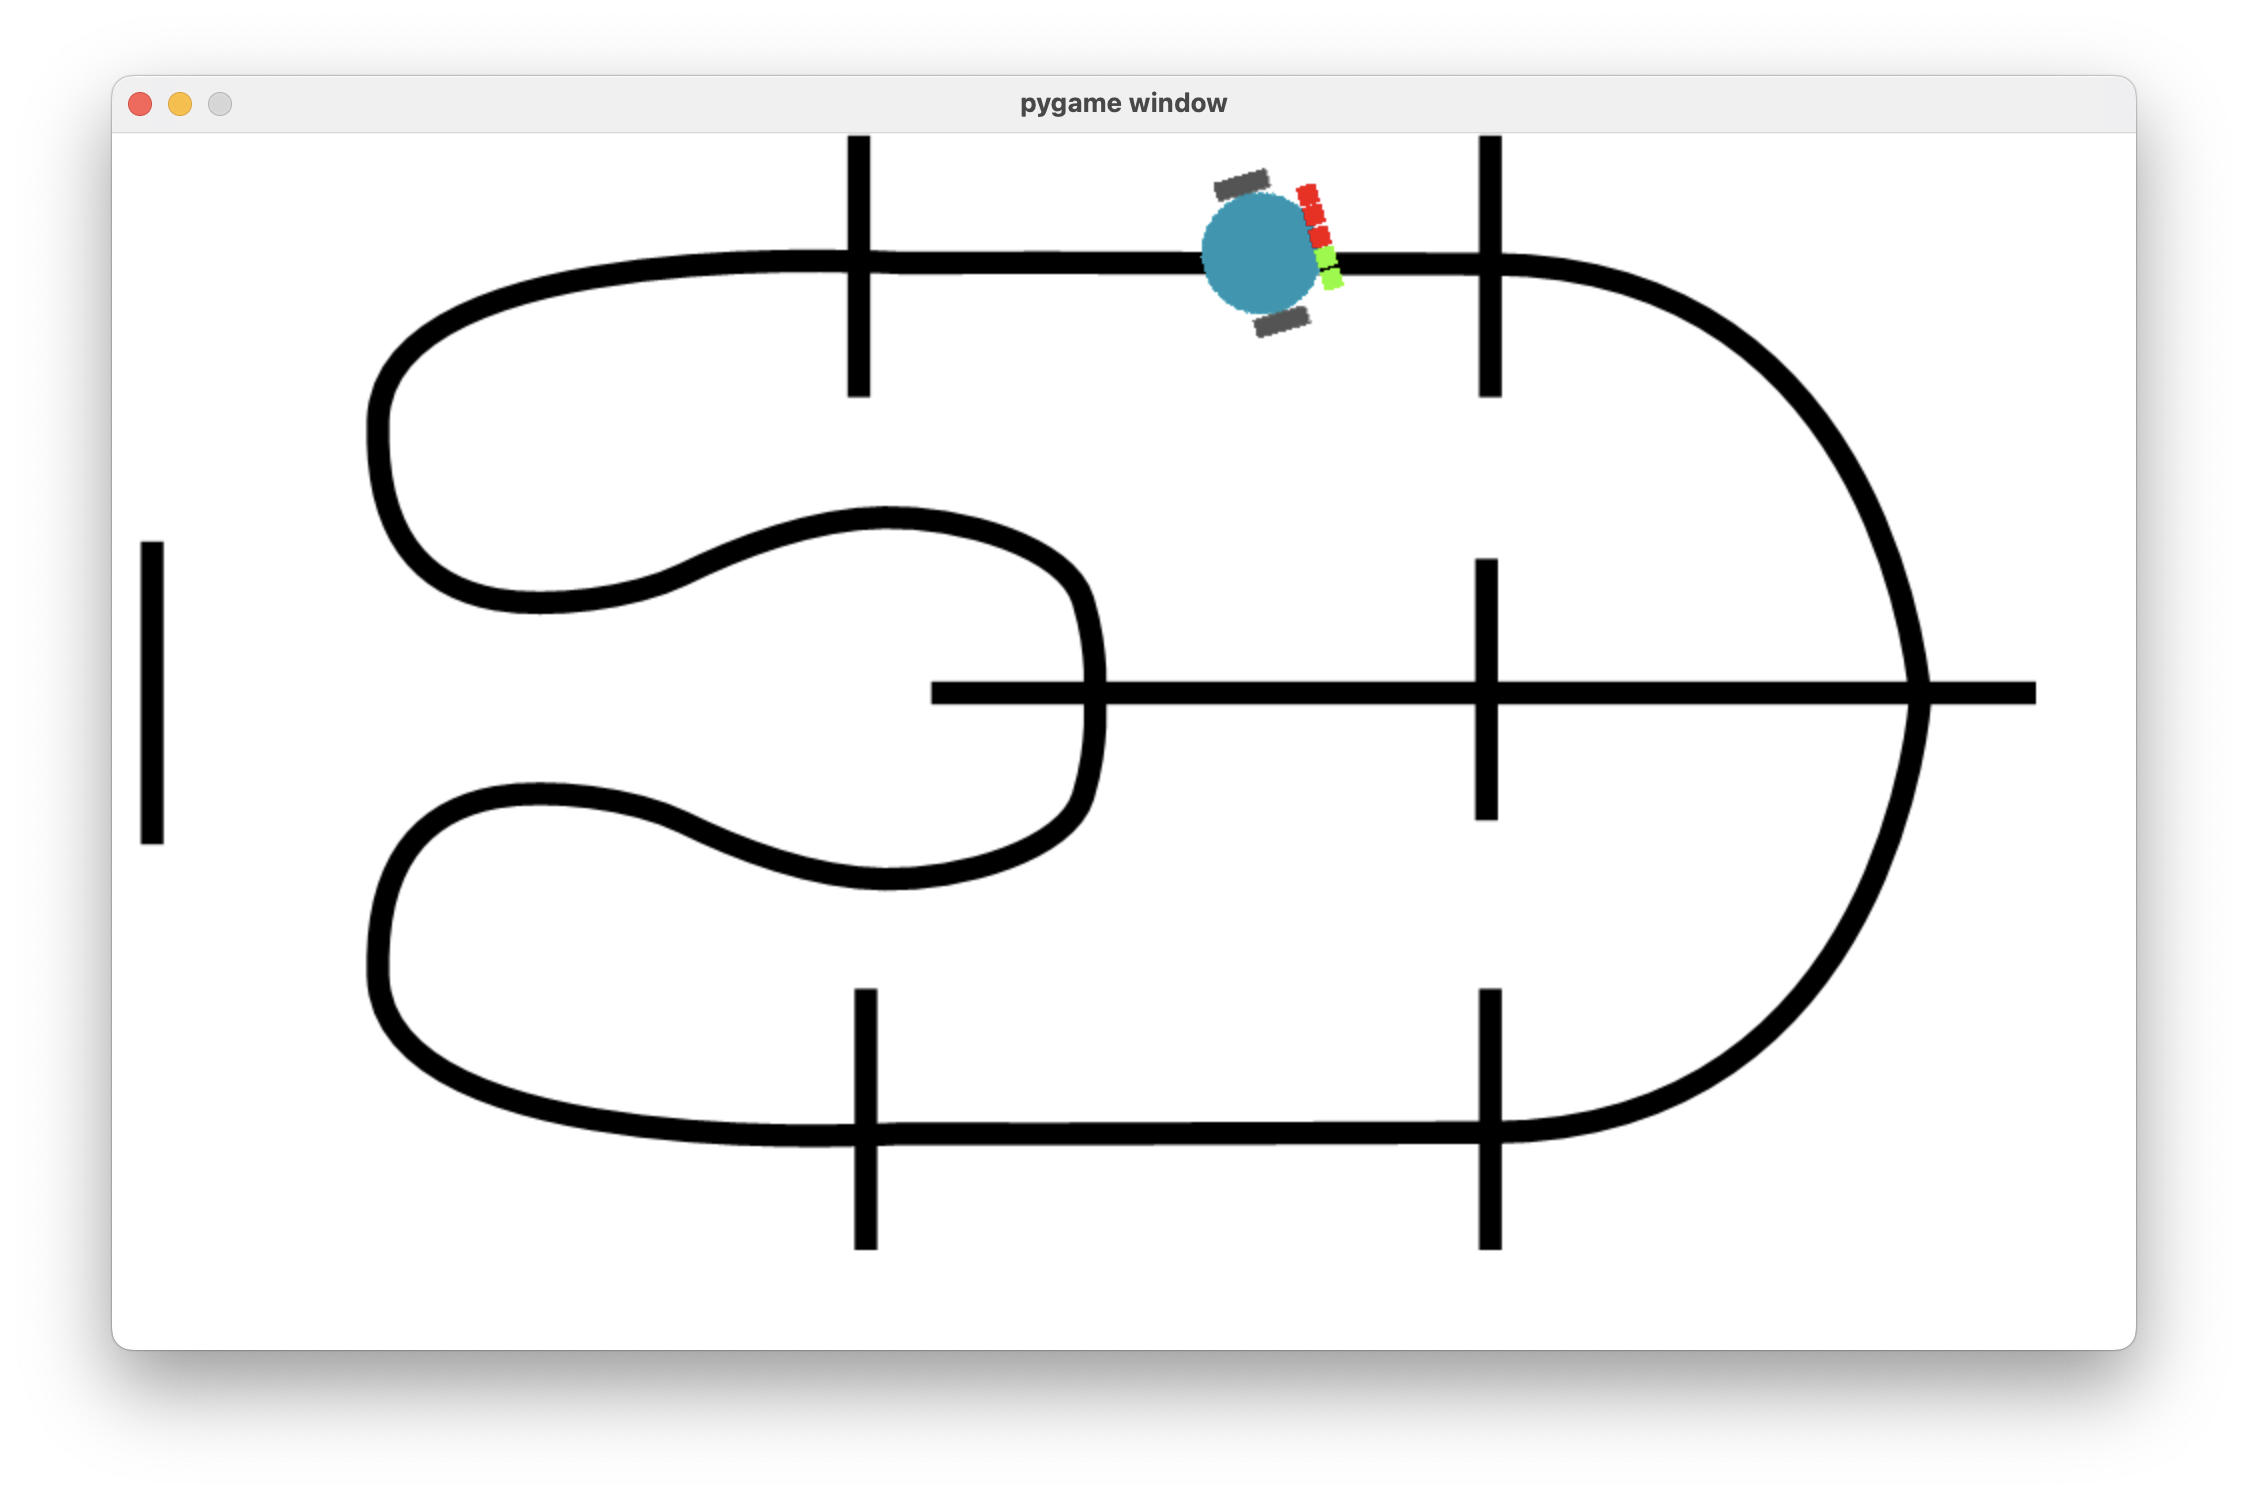
\includegraphics[width=12cm]{./imgs/PyGame.png}
\caption{Final environment developed using PyGame}
\label{fig:PyGame}

\end{figure}

\subsubsection{Process}

First, you must choose a reinforcement learning algorithm to train a neural net for your environment. In this case, PPO was used. Now the number of timesteps before saving the model and other factors regarding the learning rate must be set. The number of timesteps that I used was ten thousand. This value enabled a nice balance between training speed and small increments between saved models. Decreasing this value will increase training time as more time is wasted saving data. 
\\\\
The training can now begin; while training, the terminal will give information regarding the current performance of the agent. The mean rewards and mean time are displayed, among many other statistics. Using TensorBoard and the saved logs, the progress of a model can be graphed to monitor its performance and to debug any errors.


\subsubsection{TensorBoard}

Tensorboard is a tool developed by Google for the sole purpose of monitoring and visualizing machine learning data. Tensorboard graphs and training metrics can be viewed inside the a browser \cite{pang2020deep}. Tensorboard is used both in real-time and after training has concluded. Tensorboard will graph the mean reward and the mean time, among many others, such as loss rate.  The graph can be seen in \autoref{fig:LenTensorBoard2} and \autoref{fig:RewardTensorBoard2}.
\\\\
\begin{figure}[H]
\centering
\includegraphics[width=14cm]{./imgs/LenTensorBoard4.png}
\caption{TensorBoard graphs for mean duration over 2.5 million timesteps}
\label{fig:LenTensorBoard2}
\end{figure}
\begin{figure}[H]
\centering
\includegraphics[width=14cm]{./imgs/RewardTensorBoard4.png}
\caption{TensorBoard graphs for mean reward over 2.5 million timesteps}
\label{fig:RewardTensorBoard2}
\end{figure}
% \begin{figure}[H]
% \centering
% 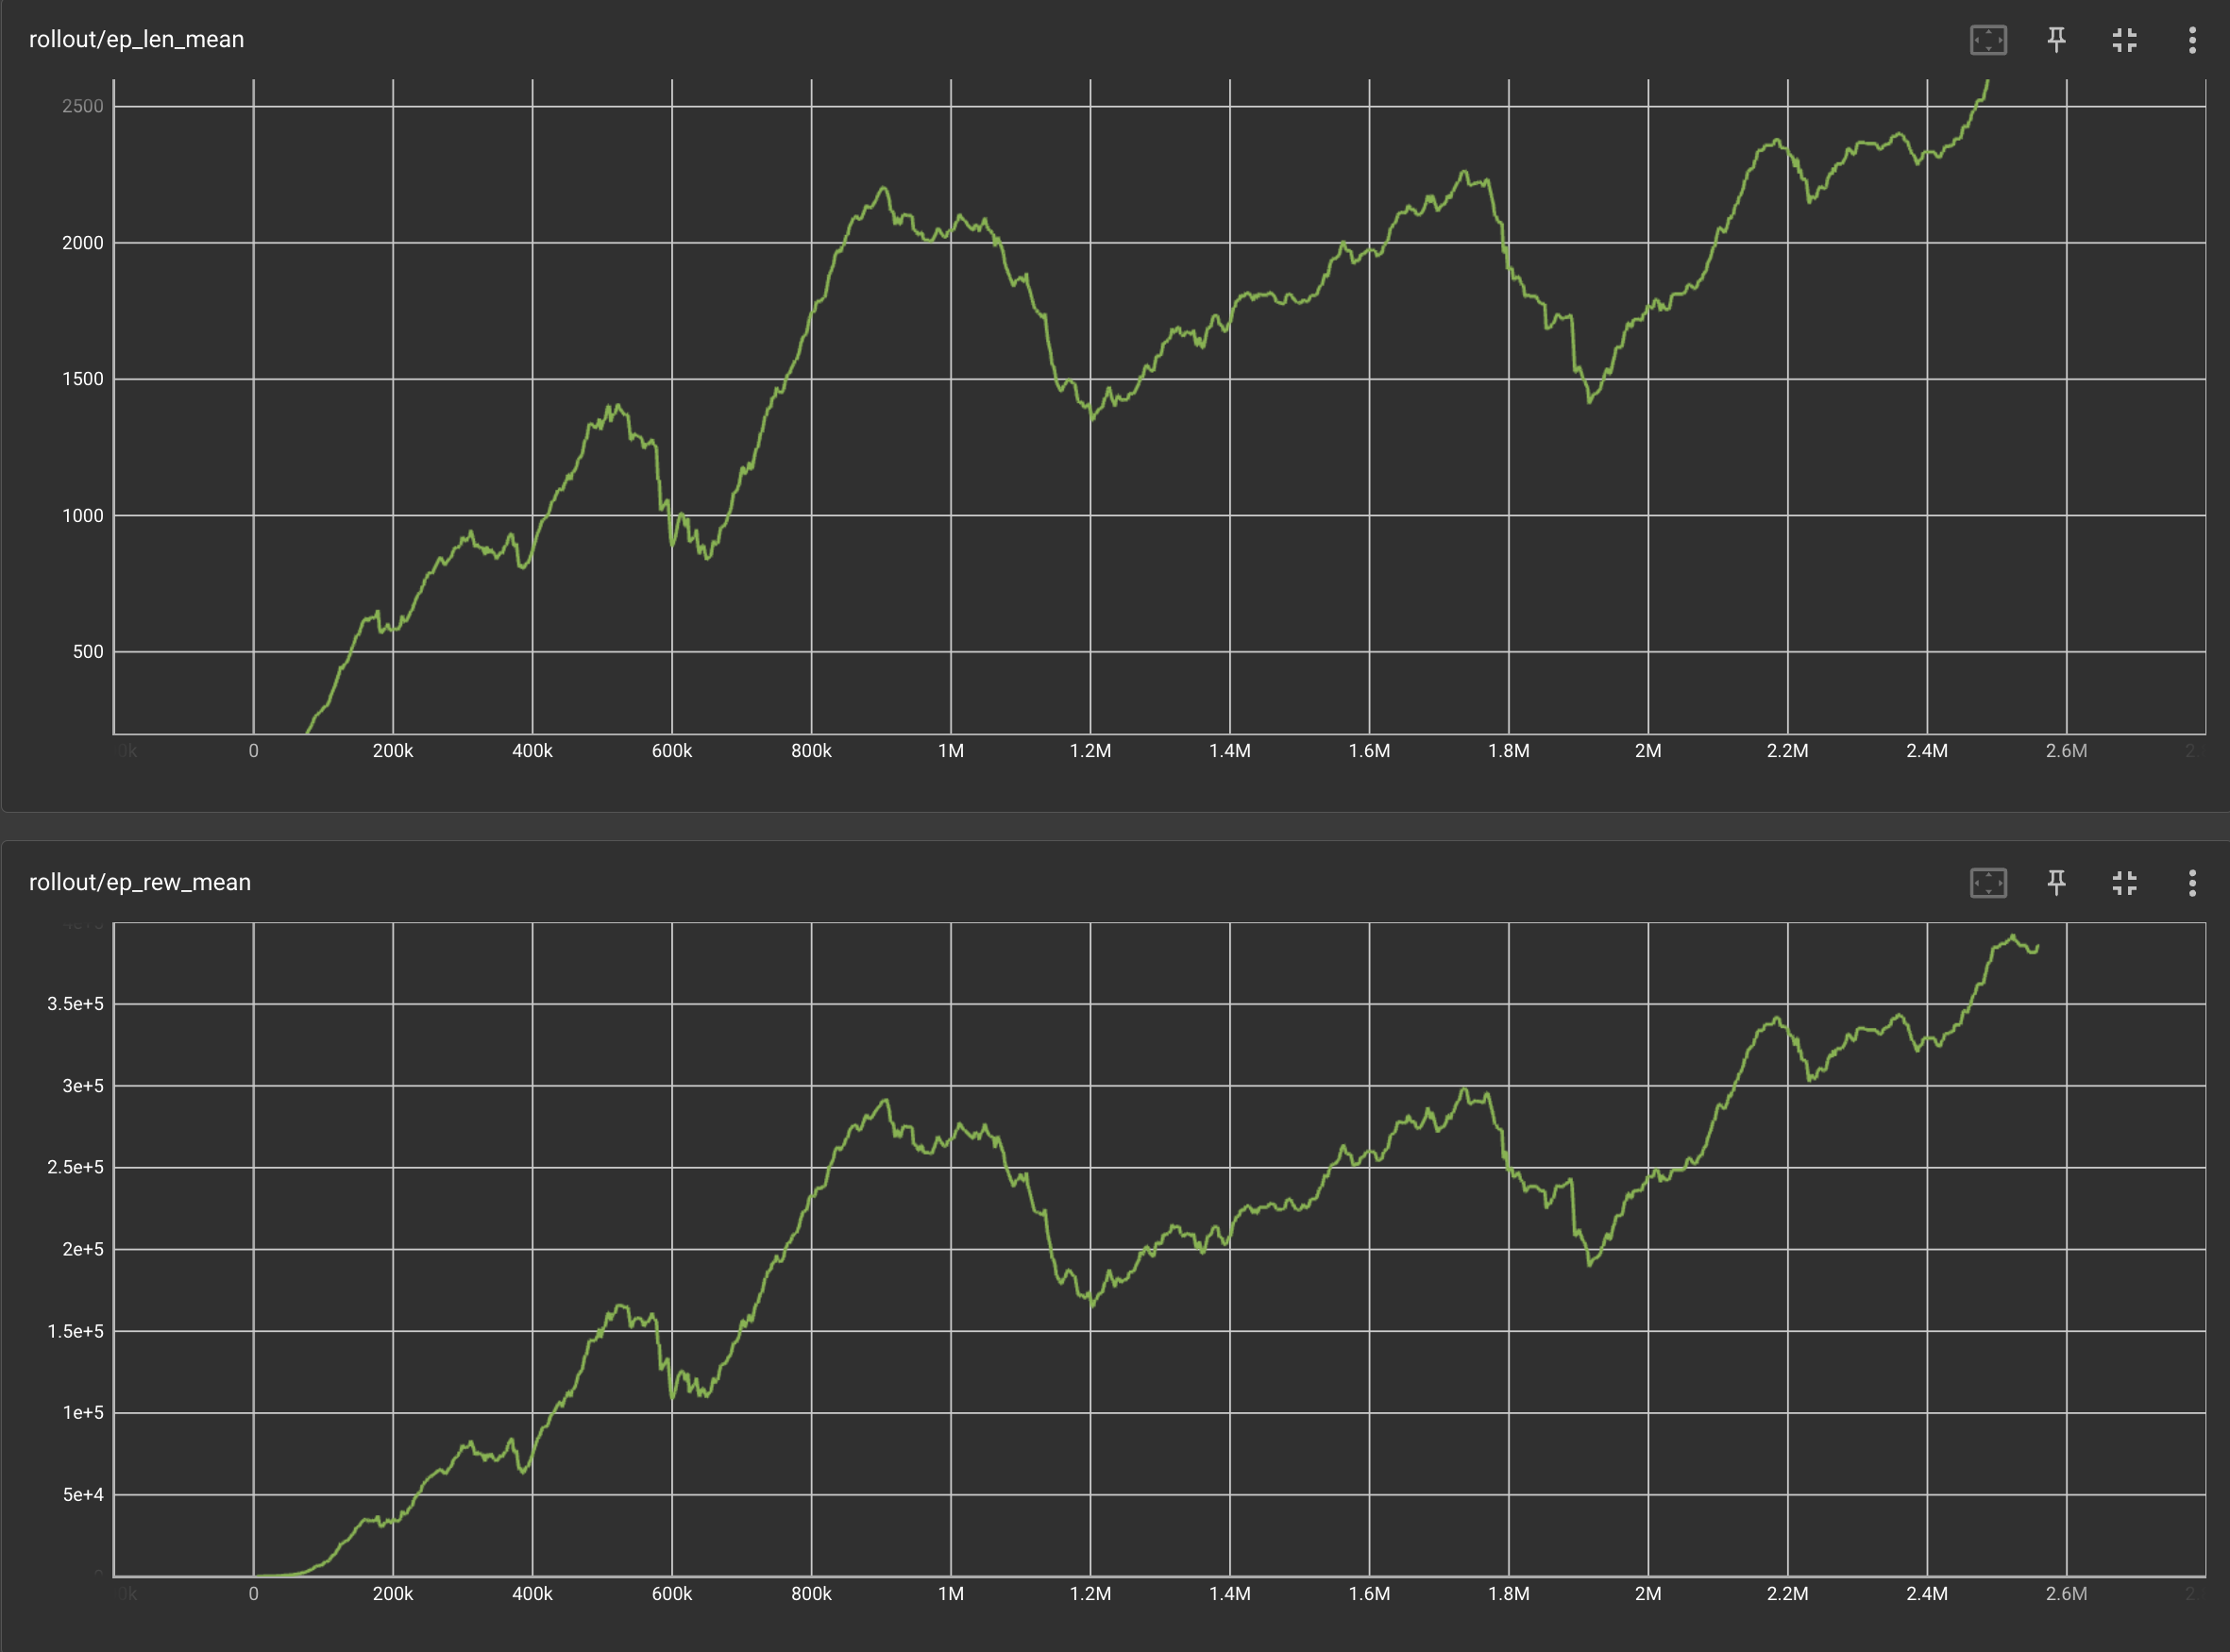
\includegraphics[width=15cm]{./imgs/TensorBoardDark.png}
% \caption{TensorBoard graphs for mean duration and reward for a PPO algorithm throughout 2.5 million timesteps}
% \label{fig:TensorBoardDark}
% \end{figure}
\noindent
Using the graph can be essential for debugging. When looking at the mean reward graph and significant dips can indicate a catastrophic failure in training. In this case, the mean time and reward functions, for the most part, looked very similar. This is because the reward system was based on the amount of time on the line. Using this information can be helpful to debug if there is a drop in reward, but the mean time continues to rise, showing a prominent issue.

\subsection{Porting to Hardware}

Porting to the MSP432 microcontroller requires three steps: neural network exporting, writing code and integration issues. By following these steps the hardware will be able to follow the line successfully. Validation at each stage should be preformed to ensure correct performance.

\subsubsection{Exporting Neural Network}
Your neural network can be exported using your saved models and a simple Python script. In order to export the neural network, the layout must first be understood. To visualise this, I converted the neural network into  Open Neural Network Exchange (ONNX) \cite{exchange2018onnx} model. ``ONNX is an open format to represent deep learning models'' \cite{lin2019onnc}. Netron, an ONNX model viewer was used to visualise. Using this, \autoref{fig:HistoryNetron} below shows the complete architecture of the trained PPO neural network.



\begin{figure}[H]
\centering{}
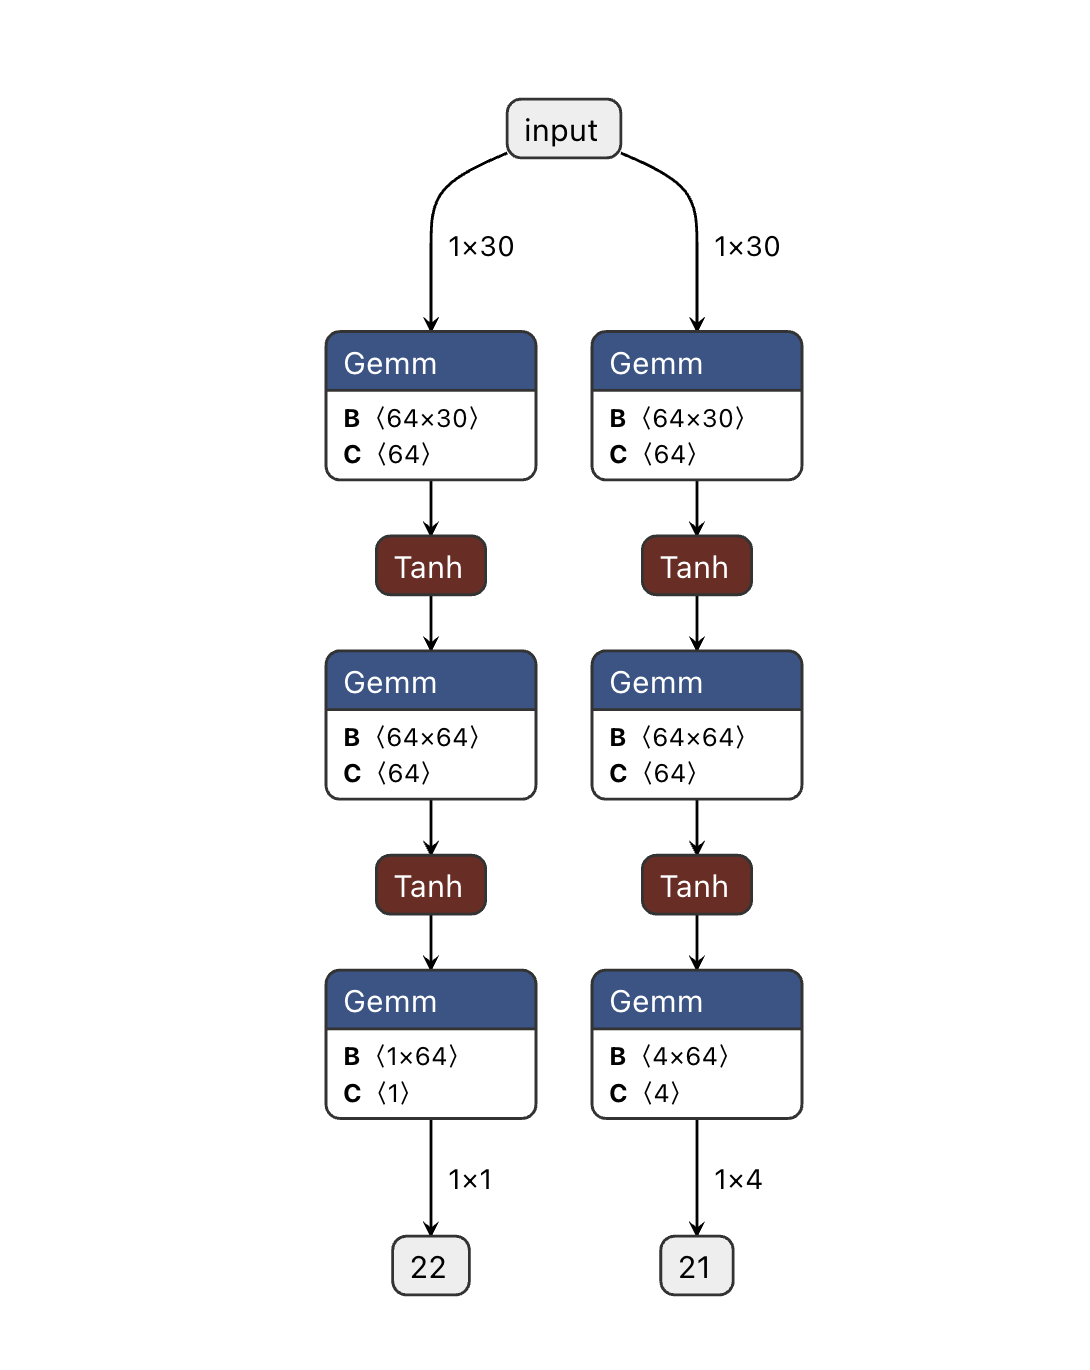
\includegraphics[width=8cm]{imgs/HistoryNetron.png}
\caption{Arcitecture of the trained PPO neural network viewed using Netron}
\label{fig:HistoryNetron}
\end{figure}
\noindent
From the figure, it can be seen that there are two sections to the network, and we are only concerned with the right-hand side. The input is an array of size thirty, and the output is an array of size four. There are two operations that are used in the neural network, the Gemm function and the Tanh function. 
\\\\
The Gemm function is comprised of two operations: matrix multiplication between matrices $A$ and $B$ and matrix addition with $C$. If the matrices are in the wrong form, the B matrix must be transposed first. The second operation is the Tanh function, which takes any value number and outputs a value within 1 and -1 bounds. Both of these equations can be seen below. 

\begin{equation}
\begin{aligned}
Y = AB^T + C
\end{aligned}
\end{equation}


\begin{equation}
\begin{aligned}
Tanh(z) = \frac{e^z-e^-^z}{e^z-e^-^z}
\end{aligned}
\end{equation}



\subsubsection{Programming Microcontroller}
Once the neural network architecture and weightings have been exported, the programming of the microcontroller can be completed. The MSP432 by Texas Instruments was used. The first element to be completed was to get the Tanh and Gemm functions working. In order to help with this, I used the MatrixMath library \cite{matrixmath}. This library contains the multiplication and the addition needed for the Gemm function. A Tanh function was then created. 
\\\\
A function can now be created to perform each element in the neural network architecture. This function executes each element in the correct order as in the model. This function will take in the observation space and output an action. 


\subsubsection{Integration Issues}

The integration issues can be solved through testing with the physical track. These issues were mainly around motor speeds, sensor calibration and microcontroller-related issues like pin allocations. 
\\\\
The first issue was to get the motors functioning properly. The motors' polarity was backward and needed to be accounted for in the code. Once this was sorted then, the speeds of the motors differed, and a ratio was acquired by lowering the faster motor. This allowed the robot to move in a straight line. 
\\\\
The second issue was the sensor calibration. The sensors work by shining an IR light at the track and then reading the reflected value through the light-dependent resistor. This value changes dramatically once a sensor leaves the line, as the black areas don't reflect as much as the white. Analysing these values is helpful in choosing a threshold for a sensor off the line. This threshold can then be used to create a function to classify if the sensor is on the line. This makes the detection of the line more accurate. 

\section{Ethics}
Reinforcement learning has many ethical considerations, including data bias, safety, privacy, transparency and environmental concerns.
\\\\
Data bias refers to the training data given to reinforcement learning. The data should be bias-free and should not try to sway the decision-making of the neural network. The neural network should be neutral towards all genders, races and demographics. Data bias was considered during this project, but there are no decisions based on humans involved in the project. The data used to train was bias-free and resulted in a fair-acting robot.
\\\\
Safety is a significant ethical consideration. An agent should be trained with the intention of avoiding any safety concerns. Regarding an agent for a self-driving vehicle, the agent should avoid collisions or any action that could result in bodily harm or damage to property. The project's safety has always been considered. The hardware itself is small, lightweight and ultimately harmless regarding collisions. Even so, the test track used walls to keep the robot confined. 
\\\\
Privacy is a principal concern when using reinforcement learning. An agent being trained using reinforcement learning should follow privacy rules and regulations. Such an agent shouldn't collect private details during or after training. This can be avoided by controlling the provided data and designing it for use ethically. This project used exclusively self-generated data to train the agent, and the data was generated depending on the action made by the agent in the simulator. The ported agent and related code used on the microcontroller don't store or train data from real life. These actions ensure privacy is kept throughout the project. 
\\\\
Transparency is vital. The logic behind the agent's action should be explainable. All of the decision-making processes should be able to be analysed through the use of a simulator or other methods to get a full in-depth understanding of the agent. It is crucial to understand how these technologies make decisions to prevent other ethical issues. Through the use of this report, the developed simulator and the provided source code, make the project entirely transparent. All of the logic behind the robot's actions can be explained through the action, observation and reward spaces. 
\\\\
Environmental concerns regarding e-waste must always be considered during any electronics project. Actions should be made to reduce, reuse and recycle electronics as much as possible. During this project, I used a line-following robot from last year. All of the parts were reused, and nothing extra was required ensuring that no e-waste was generated. 
\\\\
In conclusion, many different ethical concerns were analysed and discussed in the development of this project. All actions were taken to be as ethical as possible. I believe the project is fair to all demographics and positively impacts the development of these types of technologies. 


\section{Debugging}
During this project, there were many issues faced, and these issues ranged from code mistakes to incorrect methods. In order to recognise all of these different elements and fix each of them, debugging was performed. The two main areas where debugging occurred were in the simulator and the hardware. Each of these areas had similar issues, although the debugging styles varied significantly.

\subsection{Simulator Debugging}
When debugging the simulator, the issues were about the observation, action and reward spaces. All of these spaces could affect each other, so it was essential to keep all of these in mind whilst debugging issues. With all of these issues, the use of TensorBoard was crucial. 

\subsubsection{Debugging Observation Space}
The first point of debugging in the observation space was an issue caused by too much information in the observation space. The information in the observation space was the coordinates, angle, velocity and sensor values. The observation space can be seen in Table \ref{tab:Observation space before debugging} below.
\\\\
\begin{table}[H]
\label{table:ObsBeforeDebuggin}
\centering
\caption{Observation space before debugging}
\label{tab:Observation space before debugging}
\begin{tabular}{|ll|}
\hline
\textbf{Data Type} & \textbf{Description}\\ \hline
Double & X coordinate \\ 
Double & Y coordinate \\ 
Double & Angle\\ 
Double & Velocity of Left Motor \\ 
Double & Velocity of Right Motor \\ 
Integer & 5 Sensor values \\ \hline
\end{tabular}
\end{table}
\noindent
When training with this observation space, the mean reward graph from TensorBoard was observed, as well as running the trained model with the graphics. The training began well but quickly leveled out. The graph can be seen in \autoref{fig:LenTensorBoard1} and \autoref{fig:RewardTensorBoard1} below. By analysing the graph, it can be seen that the rewards never got high and that the mean time graph shows that the time also levelled out. This can mean several things but by looking at the model running, it can be seen that the agent is getting stuck at the first corner.
\\\\
\begin{figure}[H]
\centering
\includegraphics[width=14cm]{imgs/LenTensorBoard1.png}
\caption{TensorBoard graph for more than one hundred million timesteps. Graph showing the mean simulation time against the number of timesteps}
\label{fig:LenTensorBoard1}
\end{figure}
\begin{figure}[H]
\centering
\includegraphics[width=14cm]{imgs/RewardTensorBoard1.png}
\caption{TensorBoard graph for more than one hundred million timesteps. Graph showing the mean reward against the number of timesteps}
\label{fig:RewardTensorBoard1}
\end{figure}





% \begin{figure}[H]
% \centering
% 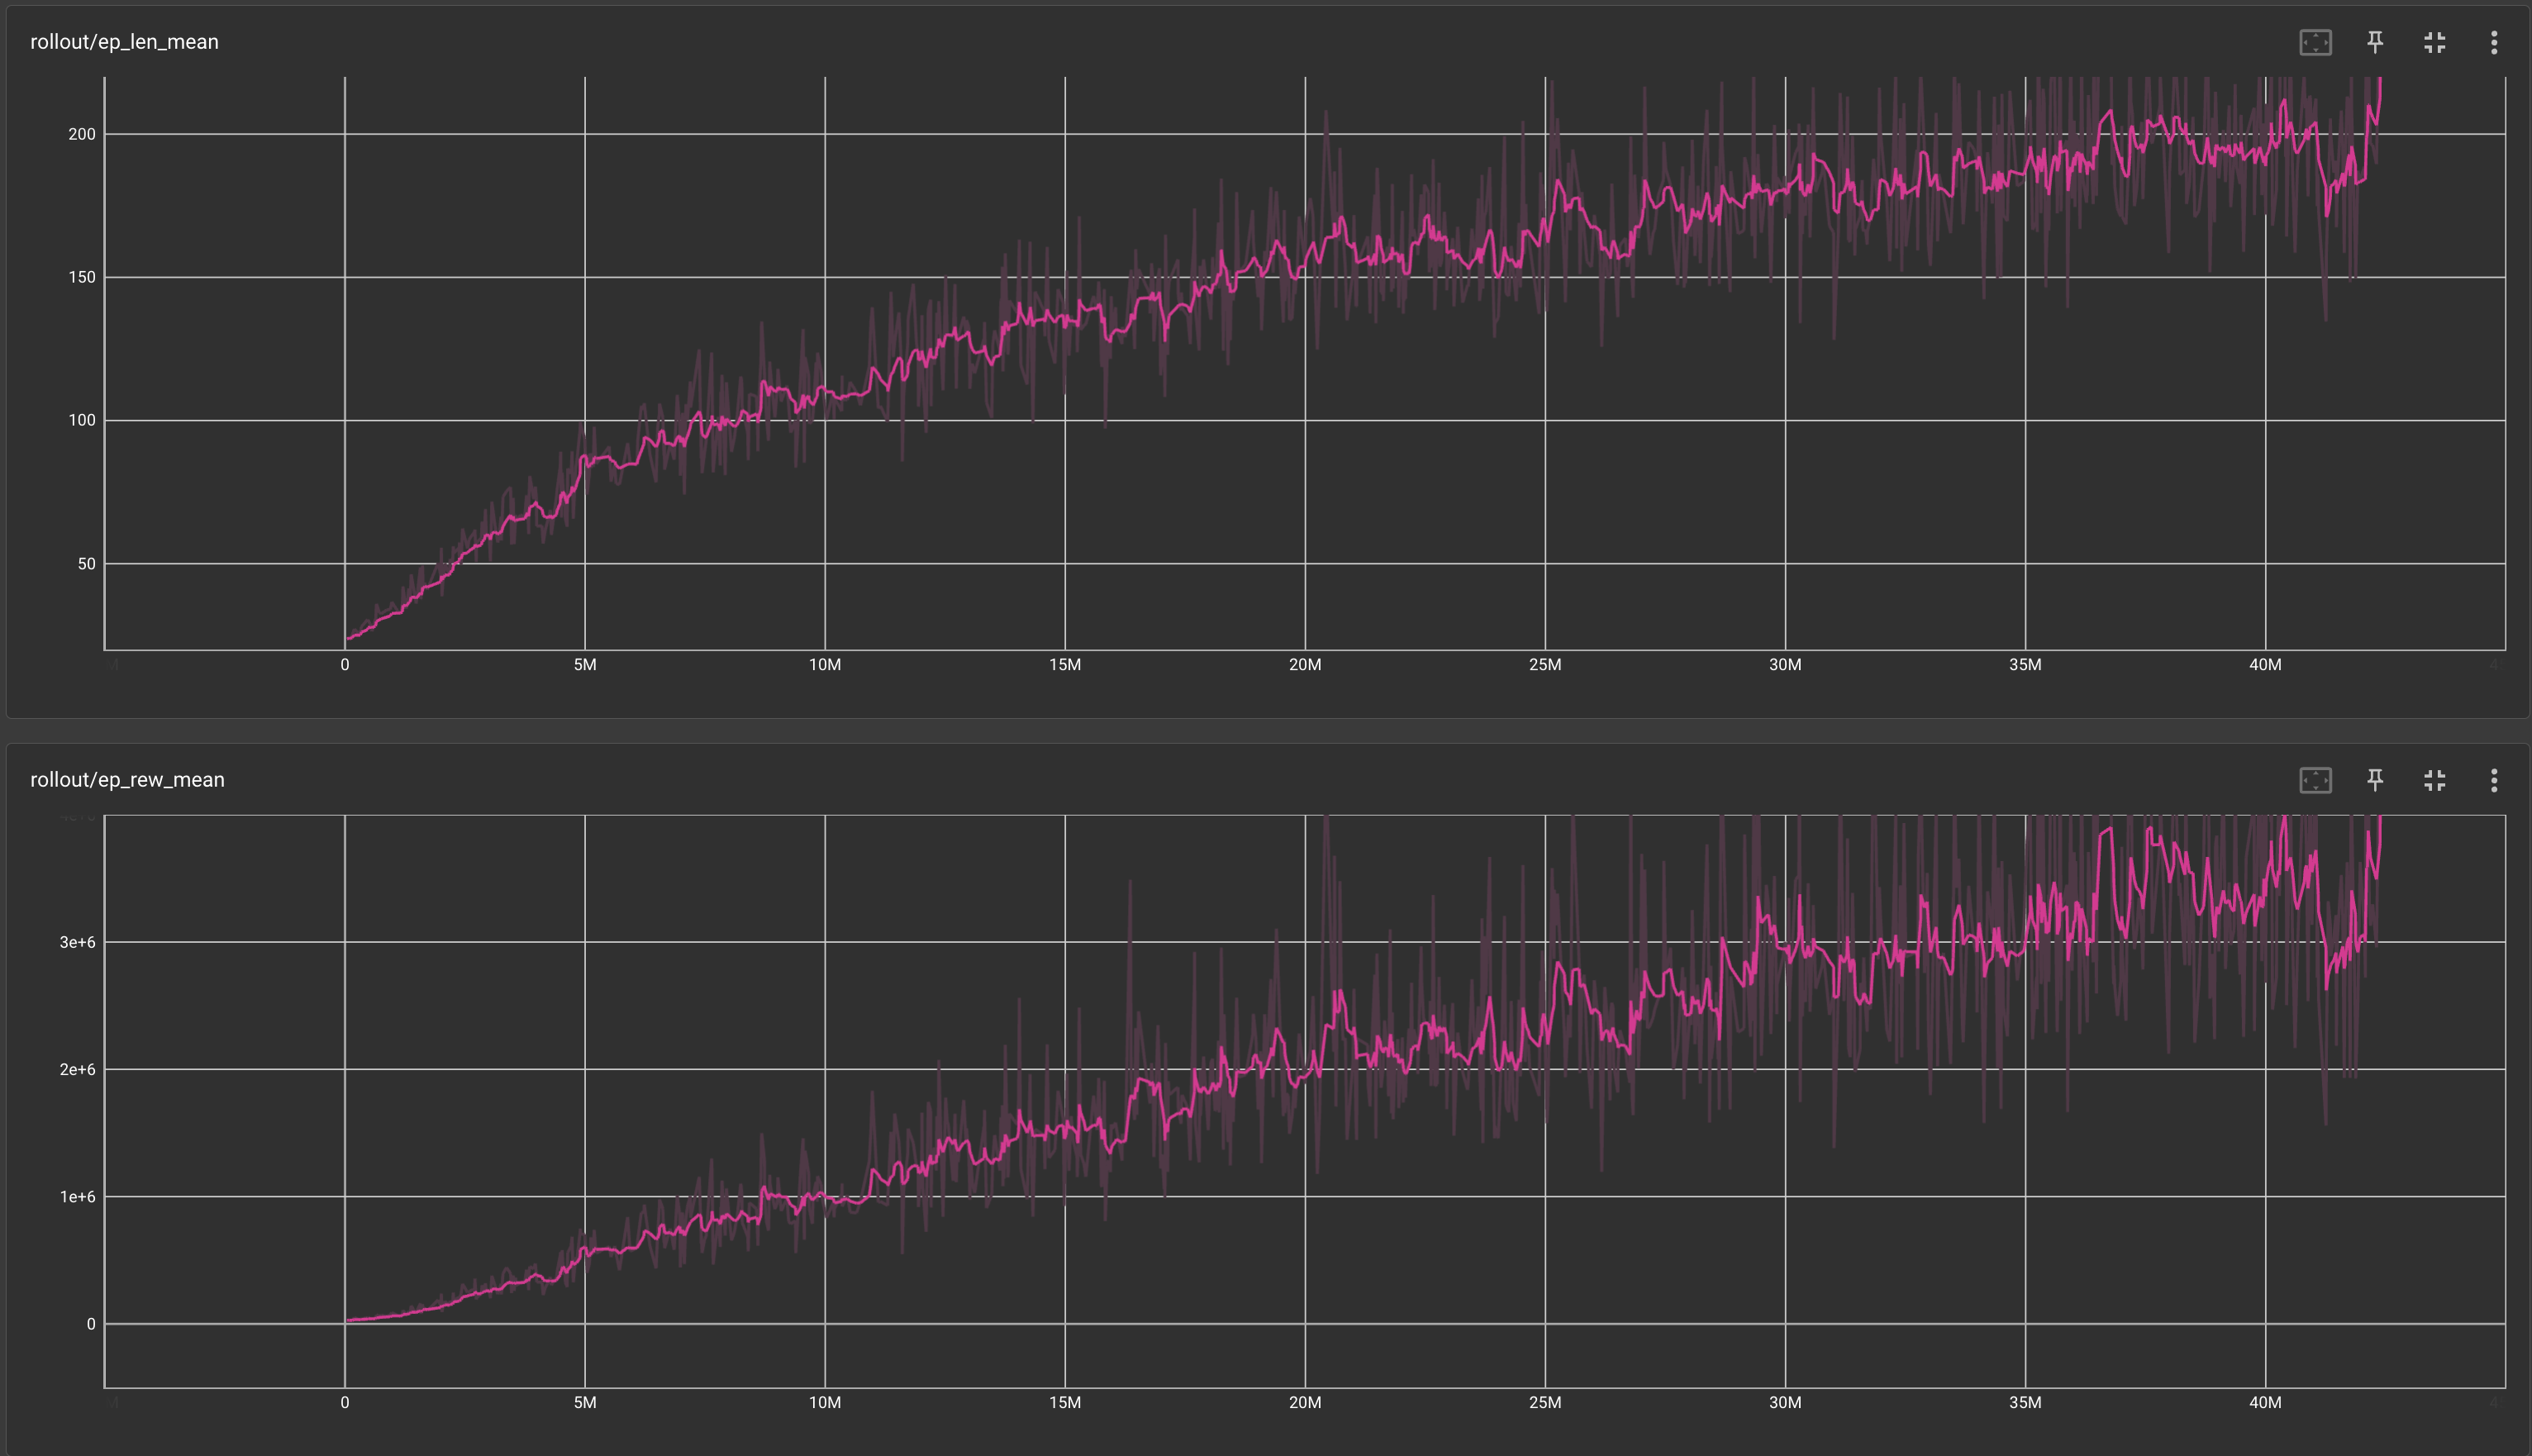
\includegraphics[width=15cm]{imgs/ObsDebugging.png}
% \caption{TensorBoard graph over forty million timesteps showing the agent getting stuck a the first corner}
% \label{fig:ObsDebugging}
% \end{figure}
\noindent
With more training, now at over twenty million time steps. The mean reward slowly increased, and with further investigation, the agent started to complete the first corner. It was clear that the observation space was too large and must have some redundant data within it. A reduction in the observation space was necessary to decrease the training time significantly. 
\\\\
The second major point of debugging was when the simplified observation space containing just the five sensor values was in use. This observation space can be seen in Table \ref{tab:Observation space containing the five sensor values} below. 
\\\\
\begin{table}[H]
\centering
\caption{Observation space containing the five sensor values}
\label{tab:Observation space containing the five sensor values}
\begin{tabular}{|ll|}
\hline
\textbf{Data Type} & \textbf{Description}\\ \hline
Integer & Sensor value 1\\ 
Integer & Sensor value 2\\ 
Integer & Sensor value 3\\ 
Integer & Sensor value 4\\ 
Integer & Sensor value 5\\ \hline
\end{tabular}
\end{table}
\noindent
During training, the model seemed to be training well, although the mean reward graph showed that a lower than expected mean reward and showed instablilty. The model was then run using graphics to monitor its actions and behaviour. The agent could follow the line and go through intersections if the robot was passing them perfectly, perpendicularly. The agent would turn at the intersections otherwise. 
\\\\
In order to solve this issue, history was added to the observation space, and this was because the agent would be able to use the history as more data to make its decisions. When the robot used only one set of sensor values, it would think it must turn, although using the history, the agent could ignore the intersection. 

\subsubsection{Debugging Action Space}
The action space had one main issue that required debugging. The issue was about the range of values being used for the motors. The action space being used was a discrete action space with a size of ten. The action space had two forward speeds, two backward speeds and a stopped. This action space can be seen below in Table \ref{tab:Discrete action space of size ten}.
\\\\
\begin{table}[H]
\centering
\caption{Discrete action space of size ten containing two forward speeds, two backward speeds and a stopped for each wheel}
\label{tab:Discrete action space of size ten}
\begin{tabular}{|ll|}
\hline
\textbf{Action} & \textbf{Description}\\ \hline
1 & Full speed forward left \\ 
2 & Half speed forward left \\ 
3 & Stopped left \\ 
4 & Half speed backward left \\ 
5 & Full speed backward left \\ 
6 & Full speed forward right \\ 
7 & Half speed forward right \\ 
8 & Stopped right \\ 
9 & Half speed backward right \\ 
10 & Full speed backward right \\ \hline
\end{tabular}
\end{table}
\noindent
When debugging this action space TensorBoard graphs were the first indication of issues. The graph showed an upward curve followed by a large spike in the mean reward and also the mean time. This behaviour is very strange and caused concern. With further investigation, running the model using graphics showed that the agent would move forward and then backwards to increase its reward. The agent was exploiting the reward function. 
\\\\
In order to rectify this event, the action space was changed to only include a stopped and forward speed for each motor. It would have been possible to alter the reward function, although that would increase its complexity unnecessarily, as reversing was not required. 

\subsubsection{Debugging Reward Space}

Debugging the reward space is less straightforward than the other spaces. There was a lot of trial and error within the debugging, and using the TensorBoard graph and running the models to see the performance was done. Analysing different reward spaces against each other to see the training speed and the overall higher reward was done. Multiple models can be seen compared to each other below in \autoref{fig:LenTensorBoard2} and \autoref{fig:RewardTensorBoard2}. 
\\\\
\begin{figure}[H]
\centering
\includegraphics[width=14cm]{imgs/LenTensorBoard2.png}
\caption{TensorBoard graph comparing different training graphs against each other. Comparing the different mean lengths of simulation over their training}
\label{fig:LenTensorBoard2}
\end{figure}
\begin{figure}[H]
\centering
\includegraphics[width=14cm]{imgs/RewardTensorBoard2.png}
\caption{TensorBoard graph comparing different training graphs against each other. Comparing the different mean rewards over their training}
\label{fig:RewardTensorBoard2}
\end{figure}
% \begin{figure}[H]
% \centering
% 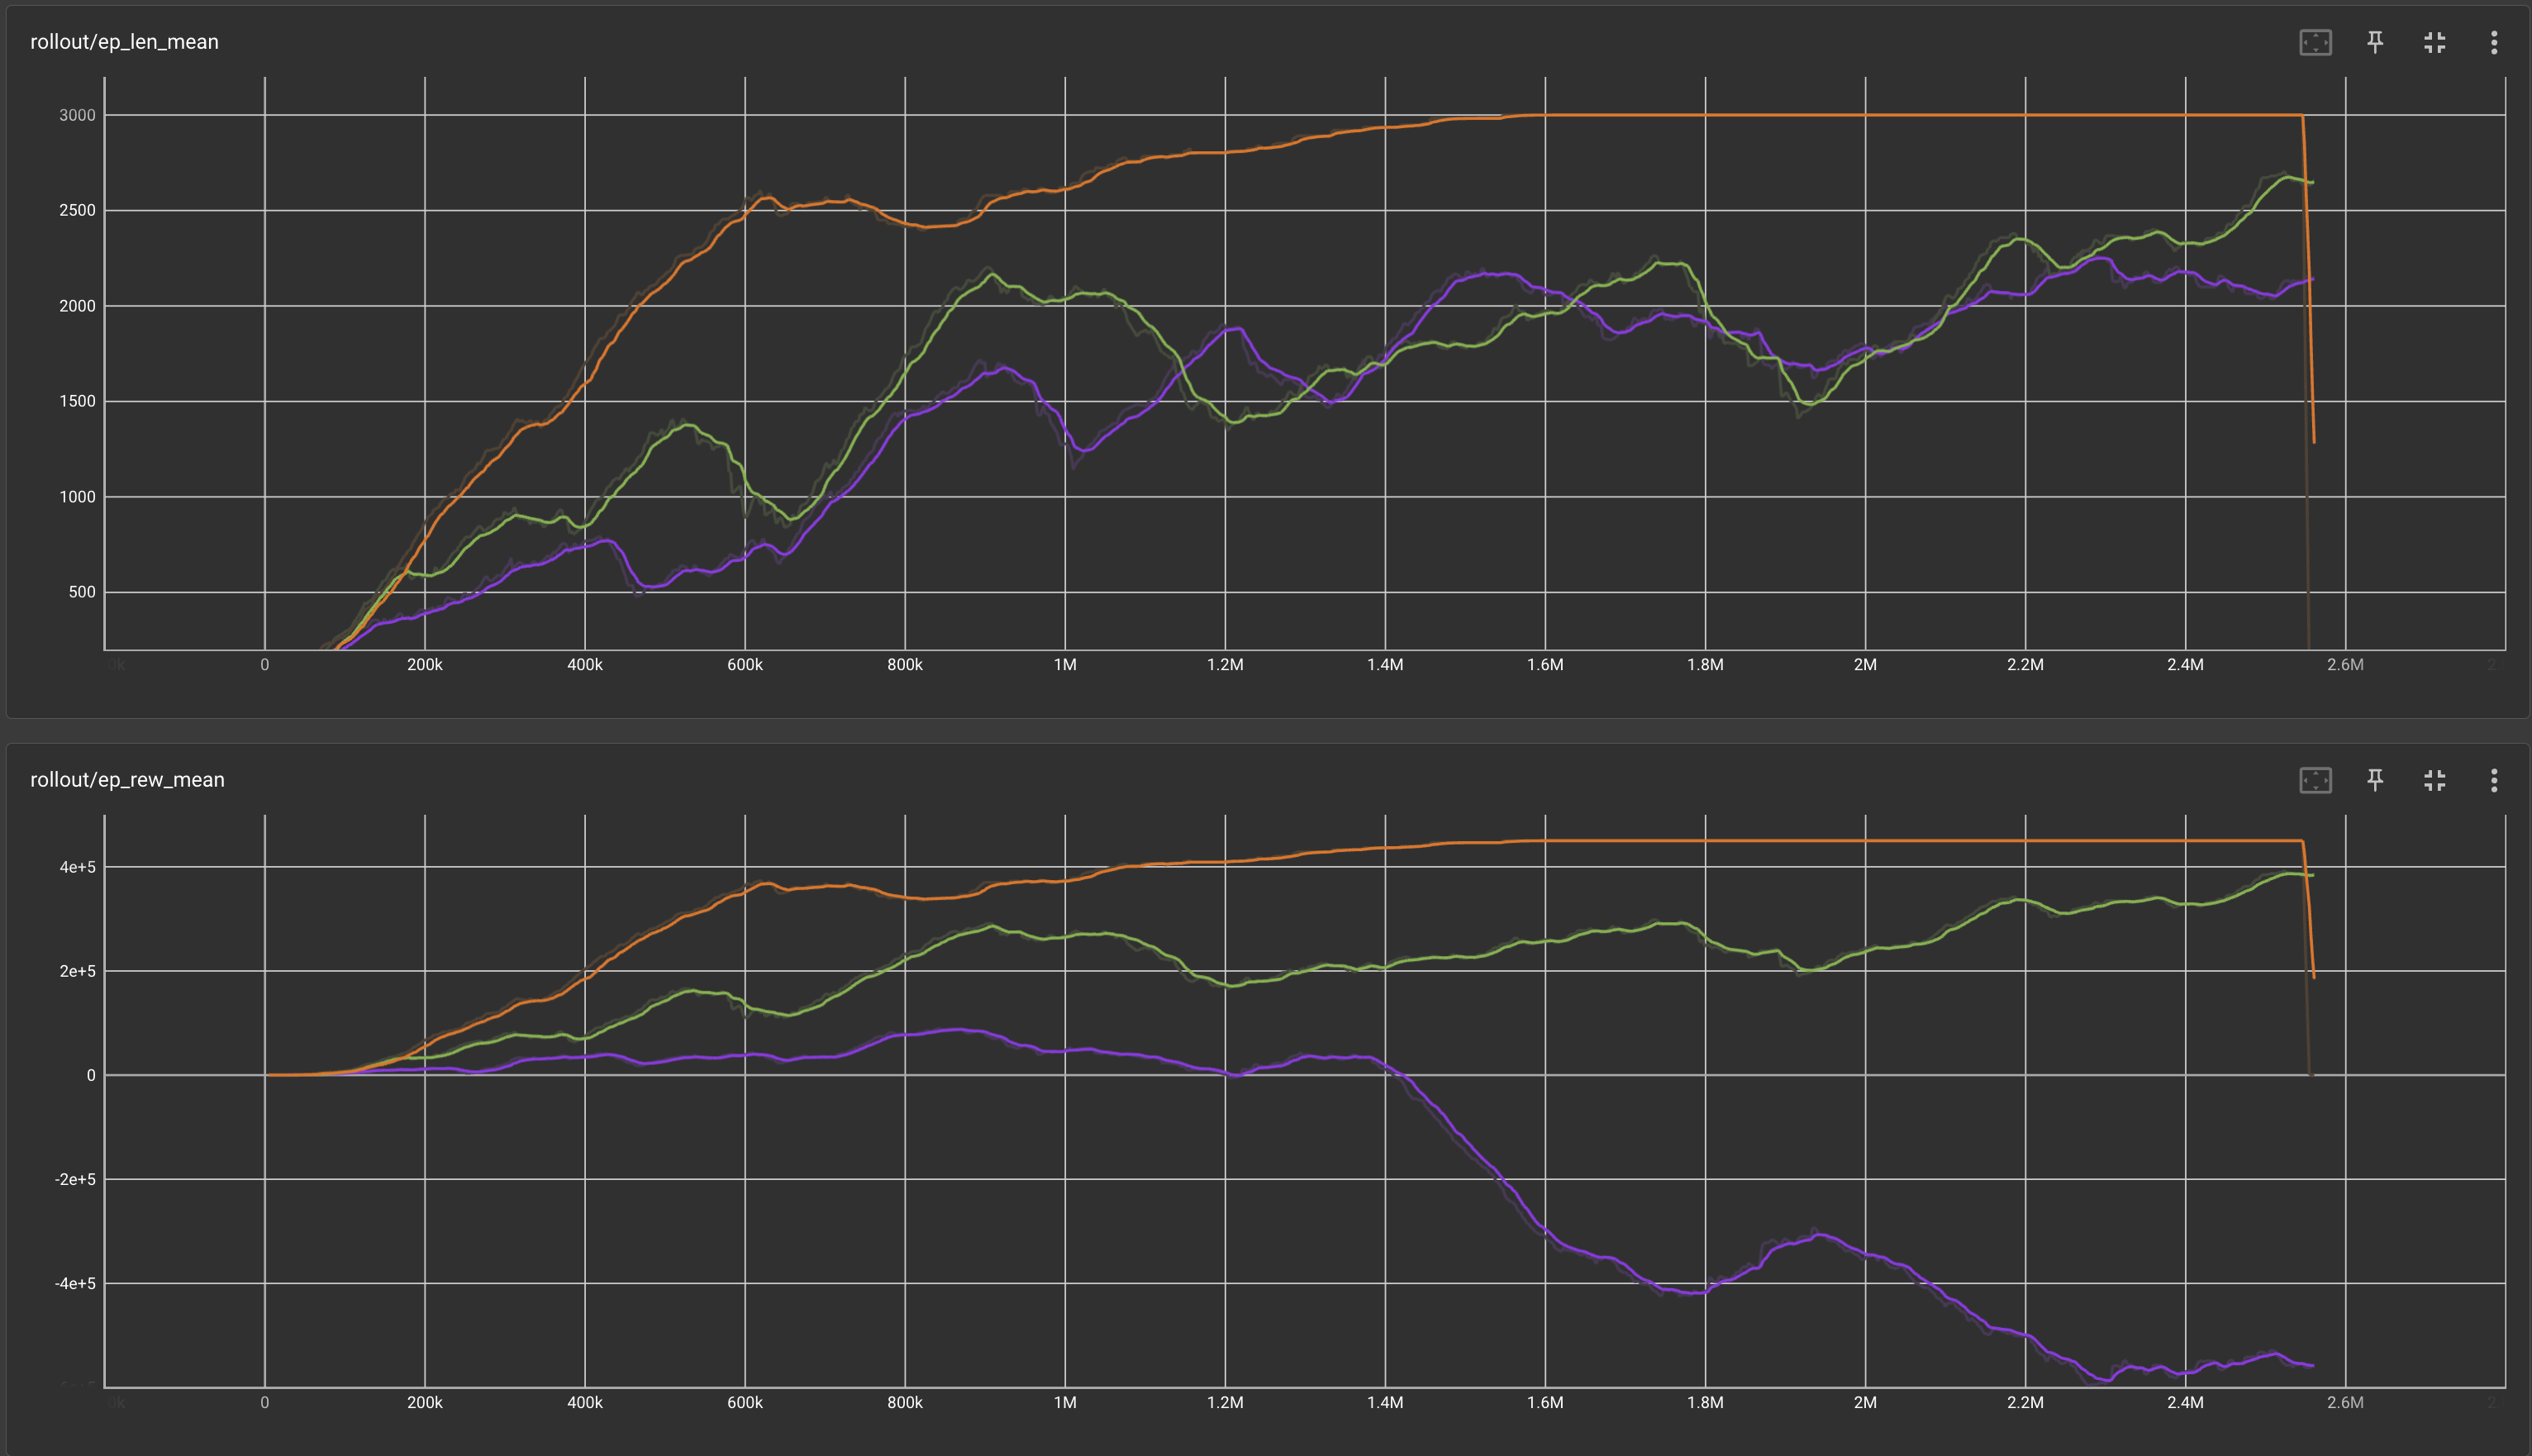
\includegraphics[width=15cm]{imgs/MultiTensorBoard.png}
% \caption{TensorBoard graph comparing different training graphs against each other}
% \label{fig:MultiTensorBoard}
\end{figure}
\noindent
In order to encourage the agent to train faster, a larger punishment for leaving the line was used. To reduce the shakiness of the agent, a slight punishment was given when the motor velocities were changed. Other methods were refined to optimise the reward space as much as possible.

\subsection{Hardware Debugging}
When debugging the hardware, there were two main areas: the matrices porting and the sensor calibrations. 
\\\\
The porting of the matrices was a significant issue. The matrices were first ported and added to the C code. These matrices were able to fit on the MSP432, although there they needed to be transposed. In order to transpose these matrices, more space was required, which caused the storage limit to be exceeded. In order to overcome this, it was necessary to transpose the matrices before adding them to the MSP432. Next, the neural network was tested, and a fixed value for the sensors was given on both the microcontroller and the original agent. This gave two different values for the action space. 
\\\\
In order to debug the problem, the matrices were examined, which were correct. Then the equation for the General Matrix Multiply (GEMM) function was examined, and the issues were found. The GEMM function is a function for small matrix multiplication and bias addition \cite{jhurani2015gemm}. There was no need for one of the matrices to be transposed. With this change in the code, another set of testing with both of the models was done. This showed the same value for the action verifying the agent was ported correctly. 
\\\\
The next element that needed doing was the sensor calibration. The sensor has two conditions, on the line and off the line. If the sensor is on the line, it will show a lower value than when the robot is off the line. In order to calibrate this, the current values of the sensors were sent to the serial port. The robot was then moved around the track to get a variety of different values. These values were examined and compared to get a threshold for the sensor being off the line. This threshold was then enforced in the code. 

\section{Testing}

% To begin testing, a metric for success must first be defined. The project's success metric is to get the simulator to train a model that can complete EE303's track without leaving the line, which should be repeatable. For the hardware, the neural network trained in the simulator should be ported over correctly, and further research should be performed to see what steps are required to get the robot to follow the line in real life.
% \\\\
% Simulator testing was performed using the trained model. The model was then run using the graphics, and the performance was analysed. In order to meet the success metric, the robot should not leave the line or cause the simulation to reset. Each simulation lasted fifty seconds.
% \\\\
% In order to test the agent on the hardware, two methods were used. The first technique used in the debugging stage, gave the ported agent a value and confirmed the same action. Secondly, the ported agent and hardware were tested using the track. This testing was done by setting the robot in random locations and allowing it to do two complete track laps, then replacing the robot. This was repeated ten times to test at multiple different locations and orientations to test all scenarios. 

To begin testing, a metric for success must first be decided. The project's success metric is to get the simulator to train a model that can complete EE303's track without leaving the line, which should be repeatable. For the hardware, the neural network trained in the simulator should be ported over correctly, and further research should be performed to see what steps are required to get the robot to follow the line in real life. 
\subsection{Simulator Testing}
Simulator testing was performed using the trained model. The model was tested using three methods. Firstly the simulator was run with the graphics enabled. This allowed for visual testing of the model. If the robot were to leave the line, this could be observed. Secondly, the performance of the model could be analysed using TensorBoard. This will examine the training progress that the model went through and can give an indication of its performance. Thirdly the trained agent will be compared to a random agent, and the average reward will be compared. Each simulation was run for a maximum time of fifty seconds.
\\\\
These tests allow valuable insight into how the simulator is performing and can quantify its performance. These simulator tests each have their own limitations. TensorBoard is able to give valuable insight into the training process, although it doesn't show all of the complexities of the neural network and its behaviour. Comparing the average reward received from the random and trained agent will show improvement, although it won't be too helpful in debugging. The simulations being run for only fifty seconds demonstrates short-term performance, although they may not show how the agent would work in the long term. 
\subsection{Hardware Testing}
In order to test the agent on the hardware, two methods were used, the technique of comparing the ported neural network to the original neural network used in the debugging stage and the testing of the robot on the track. This testing was done by setting the robot in random locations and allowing it to do two complete laps of the track, then replacing the robot. This was repeated ten times to test at multiple different locations and orientations to test all scenarios. These two methods allow for the confirmation that the neural network is working correctly and allows for visual analysis of the robot's performance.
\\\\
These tests also have their limitations, specifically the visual testing on the track. While completing this testing, there are no metrics measured, and there is no method of testing if the optimum path is being taken. Testing hundreds of times would give a greater indication of the performance.
\\\\
Although there are limitations to these tests, through the use of all of these tests, both the simulator and the ported model will be tested beyond what is necessary. Other tests could be developed in the future to analyse the specific behaviours of the neural network. 

\section{Results}

This results section has two main parts. The simulator and the hardware performance.

\subsection{Simulator Performance}
The simulator results are separated into two areas the performance of the simulator and the performance of the trained algorithm. In order to train a model, the simulator must be designed correctly. The simulator can be seen at this link: \url{https://youtu.be/zOWGv2bfYoI}. This shows the working simulators performance along with a model trained using a discrete action space, as described in the design section. 
\\\\
A second method of showing the model's performance can be displayed using the TensorBoard graphs. This model's graph can be seen below in \autoref{fig:LenTensorBoard3} and \autoref{fig:RewardTensorBoard3}. The steady rise shows that the model was training properly, and the high rise in the mean reward with under 2.6 million timesteps shows that the action, observation and reward spaces are optimized and efficient. 

\begin{figure}[H]
\centering
\includegraphics[width=14cm]{imgs/LenTensorBoard3.png}
\caption{TensorBoard showing the training progress of a discrete action spaced neural network using Proximal Policy Optimization. Showing the mean length of simulation against the total timesteps }
\label{fig:LenTensorBoard3}
\end{figure}
\begin{figure}[H]
\centering
\includegraphics[width=14cm]{imgs/RewardTensorBoard3.png}
\caption{TensorBoard showing the training progress of a discrete action spaced neural network using Proximal Policy Optimization. Showing the mean reward against the total timesteps }
\label{fig:RewardTensorBoard3}
\end{figure}

% \begin{figure}[H]
% \centering
% 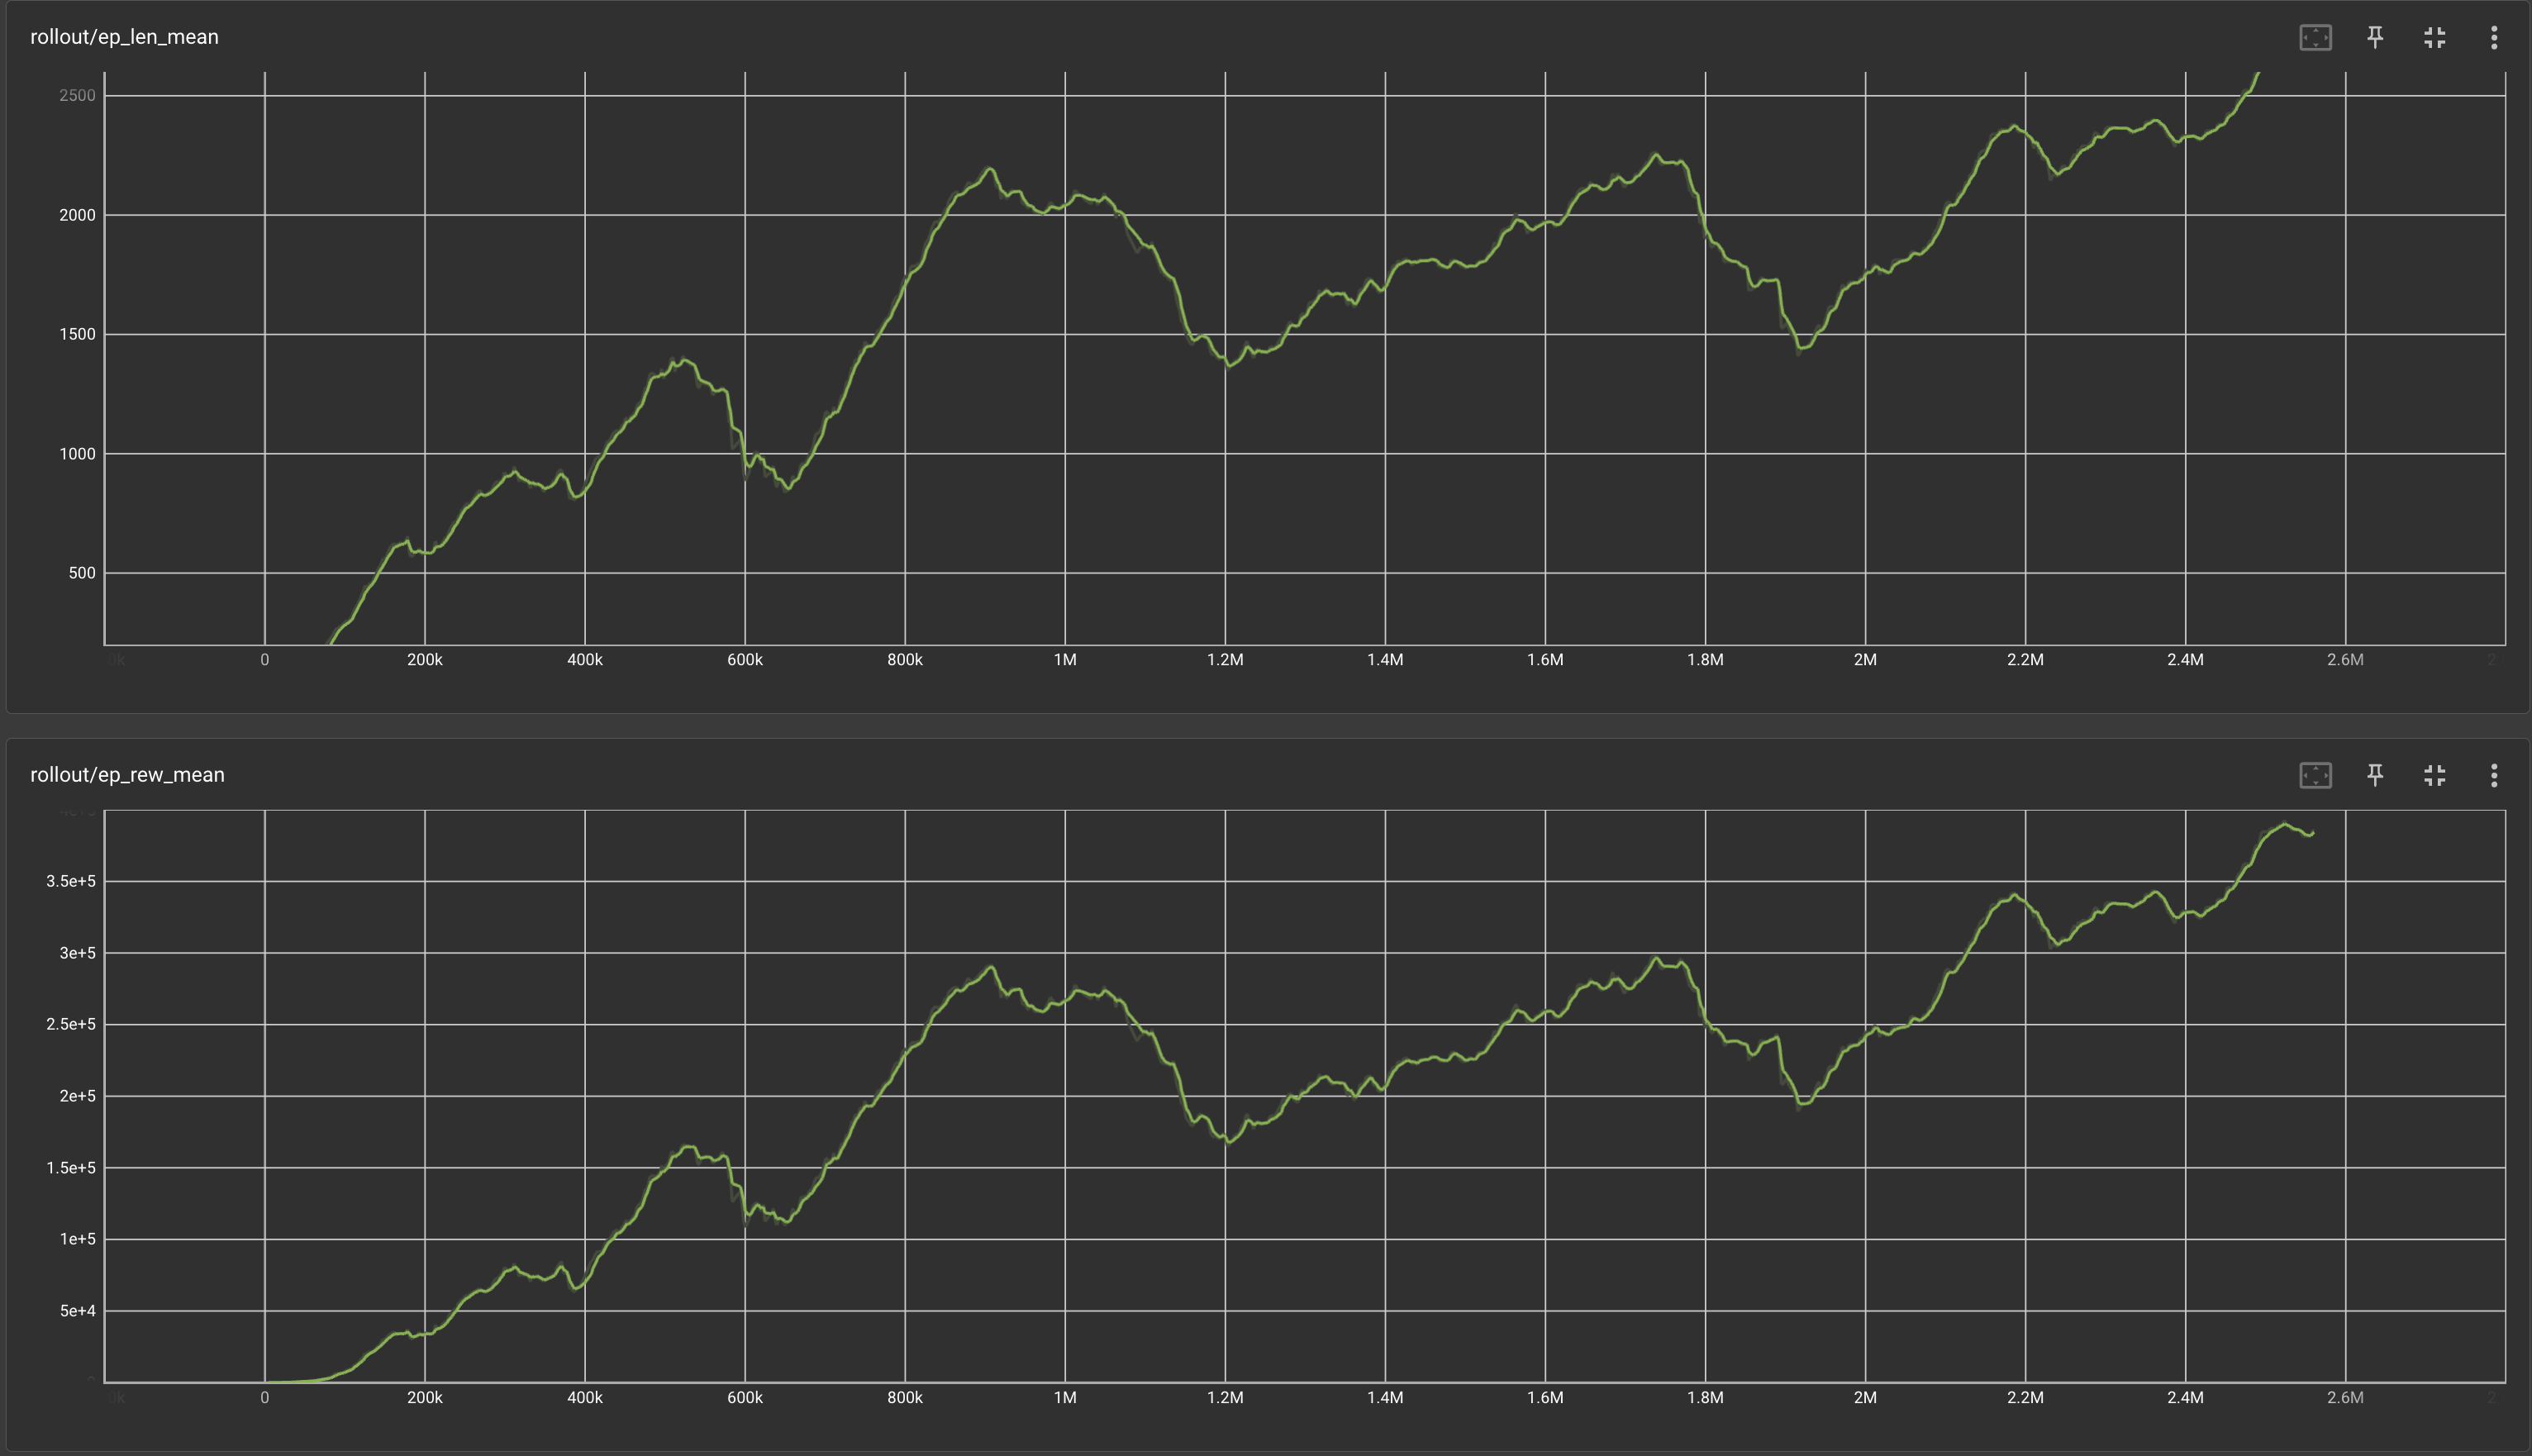
\includegraphics[width=15cm]{imgs/ResultsSimulator.png}
% \caption{TensorBoard showing the training progress of a discrete action spaced neural network using Proximal Policy Optimization. }
% \label{fig:ResultsSimulator}
% \end{figure}
\noindent
The third test comparing the trained agent to the random agent was done. This test was run twenty times for each agent and the final reward was averaged. The trained agent was able to stay on the line for the entire simulation time of ten seconds and the randomised agent would leave the line within a second. The results of the average reward can be seen in Table \ref{tab:AverageReward} and it shows that the neural network is performing far better than the random agent. 

\begin{table}[H]
\centering
\caption{Average Reward of Random and Trained neural network over a simulation time of ten seconds}
\label{tab:AverageReward}
\begin{tabular}{|ll|}
\hline
\textbf{Reward} & \textbf{Type of neural network}\\ \hline
0.532984293 & Random \\
60.00000000000058 & Trained \\
\hline
\end{tabular}
\end{table}


\subsection{Hardware Performance}
The hardware performance can be monitored in three sections. The ability to port the neural network, the ability for the robot to follow the line and the speed at which the robot can follow the line. 
\\\\
The neural network was successfully ported over to the MSP432 microcontroller and matched the performance of the trained model. This shows that the neural network was functioning properly. 
\\\\
The robot was able to follow the line accurately without leaving the line. The robot following the line can be seen at this link: \url{https://youtu.be/A_CM0yDKfE0}. The robot was able to ignore the intersections and follow all of the complex radii. 
\\\\
Finally, the robot was able to follow the line with the motors at a speed of 200 out of 255. This shows that the majority of the motor's capabilities were used. The speed of the microcontroller to process the neural network limited the speed of the motors.


\section{Conclusion}
In conclusion, the project's objective was to create a line following simulator for reinforcement learning using OpenAI Gym. The simulator was to be trained using a state-of-the-art algorithm, and its performance analysed. The neural network was then to be ported to the hardware from EE303 with the intention of performing further research into how to get the robot to follow the line. 
\\\\
Through this project, a simulator was successfully developed using OpenAI Gym and PyGame. The simulator simulated the EE303 environment. The robot's movement and sensing mechanisms were developed along with the use of the track. The simulator was used to train a neural network using a PPO reinforcement algorithm. This neural network was tested using the simulator both visually with the inbuilt graphics and through the use of analysis tools such as TensorBoard. 
\\\\
The model was ported successfully to the EE303's hardware, where it was tested against the original neural network. It matched the performance of the original. Further research was done to investigate, and the research was used to enable the robot to follow the line. The sensor calibration was completed, and the robot was tested on the EE303 track. The robot successfully followed the track without any errors. 
\\\\
The initial objectives of the project were completed successfully. In addition to meeting the initial objective, the robot was able to perform accurately on both the simulation and the track.

\subsection{Avenues for Further Research}
On completion of this project, many interesting areas could be investigated. 
\\\\
Further investigation into the line following capabilities with the intention to further optimise the robot's performance. This could reduce the necessary training time, reduce the neural network size and improve the robot's speed capabilities. This could be done by using the continuous action space and modifying the reward space to encourage the robot to complete the track as fast as possible.  
\\\\
The basic functionality of the line following robot has been created, and the rest of EE303's functionality could be investigated. The location-visiting capability of the robot could be developed using reinforcement learning. Continuing the development of the simulator to allow for the robot to initially be able to go from a start point to a specified location could be developed. This could be furthered by incorporating a wifi board and allow for a user to specify the next location. 
\\\\
The incorporation of EE303's distance sensor and additional hardware, such as a Raspberry Pi and a web camera, could be used to develop collision detection whilst following the line. The use of machine vision could be used to detect blockages in the path and prevent contact. This could look at the applications of the robot in industrial uses, such as factory transportation.

\pagebreak
\section{Project Log}
\vspace{.7cm}
\textbf{\large October 24th, 2022}
\begin{itemize}
  \item Confirmation of Project
  \item The title of the project was decided. The title is: "Differential drive mobile robot simulator for reinforcement learning"

\end{itemize}
\vspace{.7cm}
\textbf{\large October 31st, 2022}
\begin{itemize}
  \item Began collecting resource sources
  \item Read through OpenAI Gym's website

\end{itemize}
\vspace{.7cm}
\textbf{\large November 7th, 2022}
\begin{itemize}
  \item Continued resource collection
  \item Analysed examples of OpenAI Gym environments

\end{itemize}
\vspace{.7cm}
\textbf{\large November 14th, 2022}
\begin{itemize}
  \item Continued resource collection
  \item Implemented cartpole example from OpenAI Gym's example environments

\end{itemize}
\vspace{.7cm}
\textbf{\large November 21st, 2022}
\begin{itemize}
  \item Investigated Stable Baselines 3

\end{itemize}
\vspace{.7cm}
\textbf{\large November 28th, 2022}
\begin{itemize}
  \item Further Investigation into Stable Baselines 3
  \item Begun research on reinforcement learning algorithms

\end{itemize}
\vspace{.7cm}
\textbf{\large December 5th, 2022}
\begin{itemize}
  \item Trained cartpole example using PPO and DQN algorithms
  \item Analysed results from training using TensorBoard

\end{itemize}
\vspace{.7cm}
\textbf{\large December 12th, 2022}
\begin{itemize}
  \item Begun design and creation of line following environment using PyBullet

\end{itemize}
\vspace{.7cm}
\textbf{\large December 19th, 2022}
\begin{itemize}
  \item Changed from PyBullet to PyGame as PyBullet was to computationally heavy for the project.

\end{itemize}
\vspace{.7cm}
\textbf{\large December 26th, 2022}
\begin{itemize}
  \item Continued creating the environment using PyGame
  \item Created the differiental drive movement function

\end{itemize}
\vspace{.7cm}
\textbf{\large January 2nd, 2023}
\begin{itemize}
  \item Continued creating the environment using PyGame
  \item Added the images and began the collision detection

\end{itemize}
\vspace{.7cm}
\textbf{\large January 9th, 2023}
\begin{itemize}
  \item Finished the collision detection
  \item Created basic Observation Space

\end{itemize}
\vspace{.7cm}
\textbf{\large January 16th, 2023}
\begin{itemize}
  \item Created basic Reward and Action spaces

\end{itemize}
\vspace{.7cm}
\textbf{\large January 23rd, 2023}
\begin{itemize}
  \item Trained with the environment using PPO 
  \item Analysed the models using TensorBoard

\end{itemize}
\vspace{.7cm}
\textbf{\large January 30th, 2023}
\begin{itemize}
  \item Altering action, observation and reward space
  \item Analysed the models using TensorBoard


\end{itemize}
\vspace{.7cm}
\textbf{\large February 6th, 2023}
\begin{itemize}
  \item Changed the track to a simple track. This showed the first element of success
  \item Analysed the models using TensorBoard


\end{itemize}
\vspace{.7cm}
\textbf{\large February 13th, 2023}
\begin{itemize}
  \item Trianed a model to perfectly follow the track.
  \item Analysed the models using TensorBoard


\end{itemize}
\vspace{.7cm}
\textbf{\large February 20th, 2023}
\begin{itemize}
  \item Changed track to the original track without the intersections
  \item Analysed the models using TensorBoard
\end{itemize}
\vspace{.7cm}
\textbf{\large February 27th, 2023}
\begin{itemize}
  \item Changed track to original track 
  \item Analysed the models using TensorBoard
  \item Report writing 

\end{itemize}
\vspace{.7cm}
\textbf{\large March 6th, 2023}
\begin{itemize}
  \item Ported model to MSP432 
  \item Started debugging porting issues
  \item Report writing 


\end{itemize}
\vspace{.7cm}
\textbf{\large March 13th, 2023}
\begin{itemize}
  \item Finished debugging porting issues and got the robot to successfully follow the line. 
  \item Report writing 

\end{itemize}
\vspace{.7cm}
\textbf{\large March 20th, 2023}
\begin{itemize}
  \item Report writing 


\end{itemize}
\vspace{.7cm}
\textbf{\large March 27th, 2023}
\begin{itemize}
  \item Report writing 


\end{itemize}
\vspace{.7cm}
\textbf{\large April 3rd, 2023}
\begin{itemize}
  \item Report submission 


\end{itemize}

\pagebreak
\section{Appendix}
% \subsection{Software}
% \phantomsection
\subsection{Source code for the simulator and hardware}
\phantomsection
\url{https://github.com/EoinDickson/LineFollowerSim}
% \subsection{Hardware}
% \phantomsection
\subsection{MSP432}
\phantomsection
\url{https://docs.rs-online.com/3934/A700000006811369.pdf}
\subsection{Video of Simulator Working}
\phantomsection
\url{https://youtu.be/zOWGv2bfYoI}
\subsection{Video of Hardware Working}
\phantomsection
\url{https://youtu.be/A_CM0yDKfE0}


\pagebreak
\printbibliography


\end{document}